\documentclass[a4paper]{book}
\usepackage{a4wide}
\usepackage{makeidx}
\usepackage{graphicx}
\usepackage{multicol}
\usepackage{float}
\usepackage{listings}
\usepackage{color}
\usepackage{textcomp}
\usepackage{alltt}
\usepackage{times}
\usepackage{ifpdf}
\ifpdf
\usepackage[pdftex,
            pagebackref=true,
            colorlinks=true,
            linkcolor=blue,
            unicode
           ]{hyperref}
\else
\usepackage[ps2pdf,
            pagebackref=true,
            colorlinks=true,
            linkcolor=blue,
            unicode
           ]{hyperref}
\usepackage{pspicture}
\fi
\usepackage[utf8]{inputenc}
\usepackage{doxygen}
\lstset{language=C++,inputencoding=utf8,basicstyle=\footnotesize,breaklines=true,breakatwhitespace=true,tabsize=8,numbers=left }
\makeindex
\setcounter{tocdepth}{3}
\renewcommand{\footrulewidth}{0.4pt}
\begin{document}
\hypersetup{pageanchor=false}
\begin{titlepage}
\vspace*{7cm}
\begin{center}
{\Large Cinisis Database Reader }\\
\vspace*{1cm}
{\large Generated by Doxygen 1.7.1}\\
\vspace*{0.5cm}
{\small Wed Feb 23 2011 11:44:08}\\
\end{center}
\end{titlepage}
\clearemptydoublepage
\pagenumbering{roman}
\tableofcontents
\clearemptydoublepage
\pagenumbering{arabic}
\hypersetup{pageanchor=true}
\chapter{Cinisis Database Reader}
\label{index}\hypertarget{index}{}\hyperlink{classCinisis}{Cinisis} is a \href{https://secure.wikimedia.org/wikipedia/en/wiki/CDS/ISIS}{\tt CDS/ISIS} database reading library written in PHP. It's intended for integrating or migrating existing ISIS databases into other applications. It is a wrapper around other ISIS libraries and tools, providing an uniform interface and iterators for easily fetching data without bothering with internals.

\hyperlink{classCinisis}{Cinisis} works with the following ISIS backend libraries:


\begin{DoxyItemize}
\item \href{http://search.cpan.org/~dpavlin/Biblio-Isis-0.24/lib/Biblio/Isis.pm}{\tt Biblio::Isis} through \href{http://pecl.php.net/package/perl}{\tt Perl PECL extension}, which is the recommended choice.
\item \href{http://malete.org}{\tt GNI's Malete}.
\item \href{http://pecl.php.net/package/isis}{\tt Openisis}.
\end{DoxyItemize}

Both Malete and Openisis support is outdated in favour os Biblio::Isis as it has proven to be simpler and more functional.

\subsection*{Installation and usage}


\begin{DoxyVerbInclude}
Cinisis database reader
=======================

Installation
------------

### Getting Cinisis

Cinisis source code can be obtained via git:

    git clone http://git.devlet.com.br/cinisis.git

This documentation covers just installation with Biblio::Isis library
and assumes a Debian like operating system.

### Installing BiblioIsis

The Biblio:Isis can be installed directly from package together with
development files for perl:

    apt-get install libbiblio-isis-perl libperl-dev

### Installing pecl-perl

Then download and build pecl-perl:

    pecl install perl

Due to a bug (see http://pecl.php.net/bugs/bug.php?id=16807), you might
prefer to install it directly from source:

    svn checkout http://svn.php.net/repository/pecl/perl/trunk pecl-perl
    cd pecl-perl
    phpize
    ./configure
    make install

You will still need to enable the extension in your php.ini depending on
how your system is configured.

### Getting spyc

Cinisis config files are written in YAML. You'll need to download Spyc
library from https://code.google.com/p/spyc/ and put the files at
the contrib/ folder.

Configuration
-------------

  - Put your databases into the db folder, one folder per database.
  - Optionally edit config/config.yaml to set the default database.

Naming conventions
------------------

The following naming conventions are used through Cinisis aiming to help
iterating over all the data from a ISIS database.

  - Database:  an ISIS database.
  - Entry:     a given MFN in the database.
  - Value:     all the data from a given entry in the database.
  - Field:     a numbered set of values from a given entry.
  - Row:       a single value from a given field.
  - Main item: the data in a row without a qualifier.
  - Subfield:  every data in a row within a qualifier.
  - Item:      either a main item or subfield withing a row.

Example:

    MFN 1 with entry
    10: First  row of field 10^aWith a subfield^bAnd another one
    10: Second row of field 10^bJust with the second subfield
    20: This is the main item^yAnd this is another item

For that entry we have fields 10 and 20, where field 10 has two rows (i.e, two
repetitions). The main field is the data wich is has no qualifier (^) and a
subfield is the data with qualifiers (like subfields a and b from above).
\end{DoxyVerbInclude}


\subsection*{Example}

The following exemple shows how to read a database entry using two different ISIS backends:


\begin{DoxyCodeInclude}
<?php
// Import requisites.
require_once '../index.php';

// Draw the document.
$display = new CinisisDisplayHelper('Isis Reader');
$display->open_table();

$configs = array(
  0 => array(
    'implementation' => 'PhpIsis',
    'database'       => 'dbname',
  ),
  1 => array(
    'implementation' => 'BiblioIsis',
    'database'       => 'dbname',
  ),
);

foreach ($configs as $config) {
  // Get a db instance.
  $isis = new Cinisis($config);

  // Test connection.
  if ($isis->db) {
    $result  = $isis->db->read(1);
    $entries = $isis->db->entries();

    // Format output.
    echo '<td>';
    echo '<pre>';
    echo 'Implementation: '. $config['implementation'] ."\n";
    echo "Rows: $entries\n";
    print_r($result);
    echo '</pre>';
    echo '</td>';
  }
}

$display->close_table();
$display->footer();
\end{DoxyCodeInclude}
 
\chapter{Todo List}
\label{todo}
\hypertarget{todo}{}
\label{todo__todo000001}
\hypertarget{todo__todo000001}{}
 
\begin{DoxyDescription}
\item[Member \hyperlink{classIsisConnector_a10669b49c4145a86dc3662c77733d74d}{IsisConnector::existingItemKeys}(\$field, \$row=0) ]Test. 
\end{DoxyDescription}

\label{todo__todo000002}
\hypertarget{todo__todo000002}{}
 
\begin{DoxyDescription}
\item[Member \hyperlink{classMaleteDb_ad2a65876db24adc388afce465e0c153e}{MaleteDb::read}(\$id) ]Subfield handling. 
\end{DoxyDescription}

\label{todo__todo000003}
\hypertarget{todo__todo000003}{}
 
\begin{DoxyDescription}
\item[Member \hyperlink{classPhpIsisDb_af2266931746f6f2335b831be8b8333fb}{PhpIsisDb::read}(\$id) ]Subfield handling. 
\end{DoxyDescription}
\chapter{Class Index}
\section{Class Hierarchy}
This inheritance list is sorted roughly, but not completely, alphabetically:\begin{DoxyCompactList}
\item \contentsline{section}{Cinisis}{\pageref{classCinisis}}{}
\item \contentsline{section}{CinisisDisplayHelper}{\pageref{classCinisisDisplayHelper}}{}
\item \contentsline{section}{CinisisHttpHelper}{\pageref{classCinisisHttpHelper}}{}
\item \contentsline{section}{IsisDb}{\pageref{interfaceIsisDb}}{}
\begin{DoxyCompactList}
\item \contentsline{section}{BiblioIsisDb}{\pageref{classBiblioIsisDb}}{}
\item \contentsline{section}{MaleteDb}{\pageref{classMaleteDb}}{}
\item \contentsline{section}{PhpIsisDb}{\pageref{classPhpIsisDb}}{}
\end{DoxyCompactList}
\item \contentsline{section}{IsisEntryIterator}{\pageref{classIsisEntryIterator}}{}
\item \contentsline{section}{IsisItemIterator}{\pageref{classIsisItemIterator}}{}
\item \contentsline{section}{IsisMainItemIterator}{\pageref{classIsisMainItemIterator}}{}
\item \contentsline{section}{IsisMethodIterator}{\pageref{classIsisMethodIterator}}{}
\item \contentsline{section}{IsisNormalItemFilterIterator}{\pageref{classIsisNormalItemFilterIterator}}{}
\item \contentsline{section}{IsisReader}{\pageref{classIsisReader}}{}
\begin{DoxyCompactList}
\item \contentsline{section}{IsisMap}{\pageref{classIsisMap}}{}
\begin{DoxyCompactList}
\item \contentsline{section}{IsisConnector}{\pageref{classIsisConnector}}{}
\begin{DoxyCompactList}
\item \contentsline{section}{IsisFinder}{\pageref{classIsisFinder}}{}
\begin{DoxyCompactList}
\item \contentsline{section}{IsisAudit}{\pageref{classIsisAudit}}{}
\end{DoxyCompactList}
\end{DoxyCompactList}
\end{DoxyCompactList}
\end{DoxyCompactList}
\item \contentsline{section}{IsisRowIterator}{\pageref{classIsisRowIterator}}{}
\item \contentsline{section}{IsisSubfieldIterator}{\pageref{classIsisSubfieldIterator}}{}
\item \contentsline{section}{IsisValueIterator}{\pageref{classIsisValueIterator}}{}
\item \contentsline{section}{SchemaDb}{\pageref{classSchemaDb}}{}
\end{DoxyCompactList}

\chapter{Class Index}
\section{Class List}
Here are the classes, structs, unions and interfaces with brief descriptions:\begin{DoxyCompactList}
\item\contentsline{section}{\hyperlink{classBiblioIsisDb}{BiblioIsisDb} }{\pageref{classBiblioIsisDb}}{}
\item\contentsline{section}{\hyperlink{classCinisis}{Cinisis} }{\pageref{classCinisis}}{}
\item\contentsline{section}{\hyperlink{classCinisisDisplayHelper}{CinisisDisplayHelper} }{\pageref{classCinisisDisplayHelper}}{}
\item\contentsline{section}{\hyperlink{classCinisisHttpHelper}{CinisisHttpHelper} }{\pageref{classCinisisHttpHelper}}{}
\item\contentsline{section}{\hyperlink{classIsisAudit}{IsisAudit} }{\pageref{classIsisAudit}}{}
\item\contentsline{section}{\hyperlink{classIsisConnector}{IsisConnector} }{\pageref{classIsisConnector}}{}
\item\contentsline{section}{\hyperlink{interfaceIsisDb}{IsisDb} }{\pageref{interfaceIsisDb}}{}
\item\contentsline{section}{\hyperlink{classIsisEntryIterator}{IsisEntryIterator} }{\pageref{classIsisEntryIterator}}{}
\item\contentsline{section}{\hyperlink{classIsisFinder}{IsisFinder} }{\pageref{classIsisFinder}}{}
\item\contentsline{section}{\hyperlink{classIsisItemIterator}{IsisItemIterator} }{\pageref{classIsisItemIterator}}{}
\item\contentsline{section}{\hyperlink{classIsisMainItemIterator}{IsisMainItemIterator} }{\pageref{classIsisMainItemIterator}}{}
\item\contentsline{section}{\hyperlink{classIsisMap}{IsisMap} }{\pageref{classIsisMap}}{}
\item\contentsline{section}{\hyperlink{classIsisMethodIterator}{IsisMethodIterator} }{\pageref{classIsisMethodIterator}}{}
\item\contentsline{section}{\hyperlink{classIsisNormalItemFilterIterator}{IsisNormalItemFilterIterator} }{\pageref{classIsisNormalItemFilterIterator}}{}
\item\contentsline{section}{\hyperlink{classIsisReader}{IsisReader} }{\pageref{classIsisReader}}{}
\item\contentsline{section}{\hyperlink{classIsisRowIterator}{IsisRowIterator} }{\pageref{classIsisRowIterator}}{}
\item\contentsline{section}{\hyperlink{classIsisSubfieldIterator}{IsisSubfieldIterator} }{\pageref{classIsisSubfieldIterator}}{}
\item\contentsline{section}{\hyperlink{classIsisValueIterator}{IsisValueIterator} }{\pageref{classIsisValueIterator}}{}
\item\contentsline{section}{\hyperlink{classMaleteDb}{MaleteDb} }{\pageref{classMaleteDb}}{}
\item\contentsline{section}{\hyperlink{classPhpIsisDb}{PhpIsisDb} }{\pageref{classPhpIsisDb}}{}
\item\contentsline{section}{\hyperlink{classSchemaDb}{SchemaDb} }{\pageref{classSchemaDb}}{}
\end{DoxyCompactList}

\chapter{Class Documentation}
\hypertarget{classBiblioIsisDb}{
\section{BiblioIsisDb Class Reference}
\label{classBiblioIsisDb}\index{BiblioIsisDb@{BiblioIsisDb}}
}
Inheritance diagram for BiblioIsisDb:\begin{figure}[H]
\begin{center}
\leavevmode
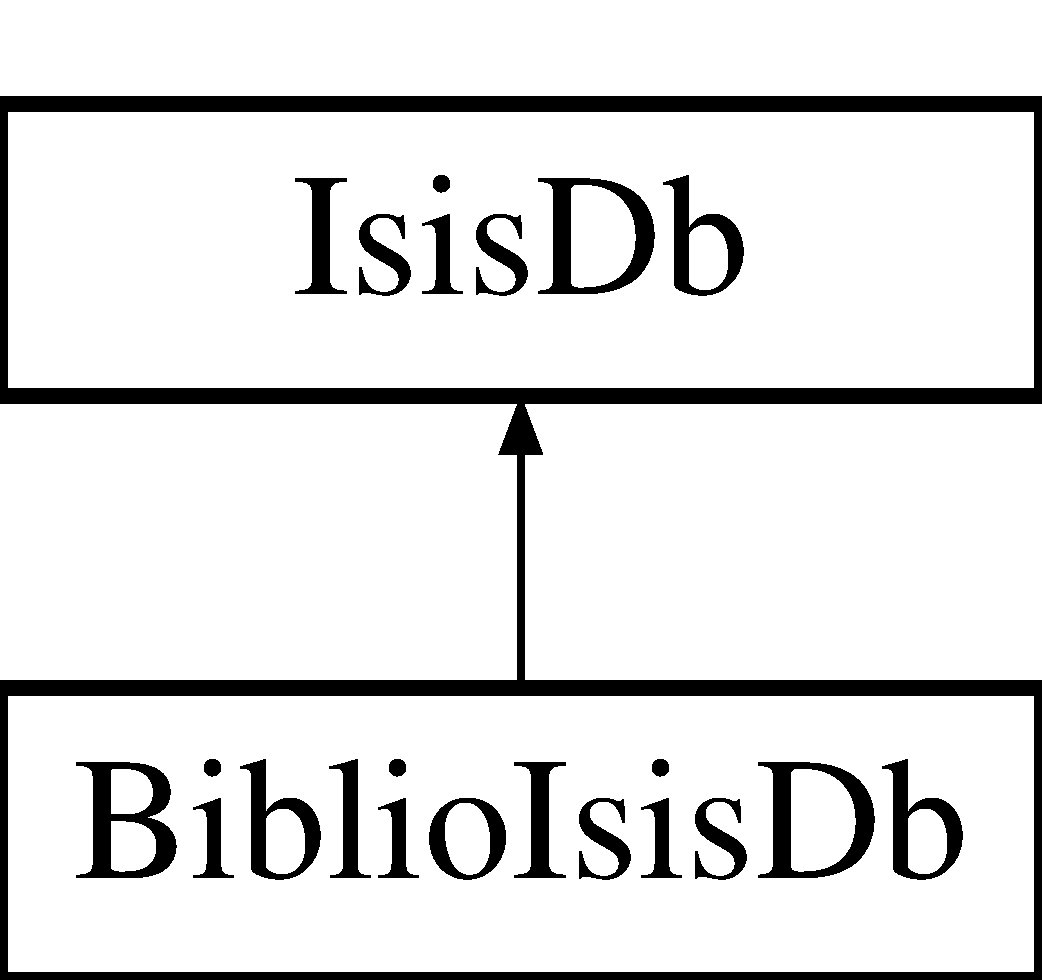
\includegraphics[height=2.000000cm]{classBiblioIsisDb}
\end{center}
\end{figure}
\subsection*{Public Member Functions}
\begin{DoxyCompactItemize}
\item 
\hyperlink{classBiblioIsisDb_ab2c5ec782b324847e104d8ad35a230af}{\_\-\_\-construct} (\$schema)
\item 
\hyperlink{classBiblioIsisDb_a286fb16de5797785d28021068efca561}{logger} (\$message)
\item 
\hyperlink{classBiblioIsisDb_ad5704f5c9454ac053e66a489797ba221}{backend} (\$method= 'count', \$args=NULL)
\item 
\hyperlink{classBiblioIsisDb_a808cdbc0d4c8f62a1465e74064f4422f}{read} (\$id, \$method= 'fetch')
\item 
\hyperlink{classBiblioIsisDb_ab6b0a977c066c25c6bdca5c1d3a083e8}{entries} ()
\item 
\hyperlink{classBiblioIsisDb_a8e76b289b9e3a9893b9469094753d2bc}{example} ()
\item 
\hyperlink{classBiblioIsisDb_a34483b463d81ba1d8031576b5735efbc}{tag} (\$results, \$method= 'fetch')
\item 
\hyperlink{classBiblioIsisDb_a73d5d998f9ab7e410c5f71f65e83948b}{has\_\-subfields} (\$key)
\item 
\hyperlink{classBiblioIsisDb_af0be305b211b96dcb4aeb8452c8331a9}{subfields\_\-switch} (\$key, \&\$value)
\item 
\hyperlink{classBiblioIsisDb_a450e26ae0b7f4967d8e25c9a3d023c75}{subfields} (\$name, \$key, \$method)
\item 
\hyperlink{classBiblioIsisDb_a8c6a0081c5296a6db520e98998502ef7}{subfields\_\-from\_\-to\_\-hash} (\$name, \$key)
\item 
\hyperlink{classBiblioIsisDb_a2b08c6a7ba20f6f5eb07edb2b4a914c1}{subfields\_\-from\_\-fetch} (\$name, \$key)
\item 
\hyperlink{classBiblioIsisDb_aa86380f9e66ea8f175c50675d1fe0a88}{is\_\-repetitive} (\$field, \$value)
\item 
\hyperlink{classBiblioIsisDb_a04089d61ce04b18aa6a78c94ca02edb9}{repetition} (\$key, \$value)
\item 
\hyperlink{classBiblioIsisDb_a2b6fd7b7316f63ac5649ebf3947c4fae}{charset} (\&\$data)
\end{DoxyCompactItemize}
\subsection*{Static Public Member Functions}
\begin{DoxyCompactItemize}
\item 
static \hyperlink{classBiblioIsisDb_a929467f1907d3aeaeebe493f0c188c5b}{check} (\$schema, \$section=NULL)
\end{DoxyCompactItemize}
\subsection*{Public Attributes}
\begin{DoxyCompactItemize}
\item 
\hyperlink{classBiblioIsisDb_a978a9243ea53b1f2426115d7b4191b07}{\$fdt}
\item 
\hyperlink{classBiblioIsisDb_a7eccfa964dcd1469a263340447c38143}{\$perl}
\item 
\hyperlink{classBiblioIsisDb_ab9fb3b6f10d2734a198ca7802ee38c2d}{\$format}
\item 
\hyperlink{classBiblioIsisDb_a67337d78af0fc21d0ff10471aa638c62}{\$log}
\end{DoxyCompactItemize}


\subsection{Detailed Description}
Biblio::Isis implementation of \hyperlink{interfaceIsisDb}{IsisDb}. 

\subsection{Constructor \& Destructor Documentation}
\hypertarget{classBiblioIsisDb_ab2c5ec782b324847e104d8ad35a230af}{
\index{BiblioIsisDb@{BiblioIsisDb}!\_\-\_\-construct@{\_\-\_\-construct}}
\index{\_\-\_\-construct@{\_\-\_\-construct}!BiblioIsisDb@{BiblioIsisDb}}
\subsubsection[{\_\-\_\-construct}]{\setlength{\rightskip}{0pt plus 5cm}BiblioIsisDb::\_\-\_\-construct (
\begin{DoxyParamCaption}
\item[{\$}]{ schema}
\end{DoxyParamCaption}
)}}
\label{classBiblioIsisDb_ab2c5ec782b324847e104d8ad35a230af}
Constructor.

\begin{DoxySeeAlso}{See also}
\hyperlink{interfaceIsisDb_ae1c0a3496d55f710d34c5c19ada7a66b}{IsisDb::\_\-\_\-construct()} 
\end{DoxySeeAlso}


Implements \hyperlink{interfaceIsisDb_ae1c0a3496d55f710d34c5c19ada7a66b}{IsisDb}.



\subsection{Member Function Documentation}
\hypertarget{classBiblioIsisDb_ad5704f5c9454ac053e66a489797ba221}{
\index{BiblioIsisDb@{BiblioIsisDb}!backend@{backend}}
\index{backend@{backend}!BiblioIsisDb@{BiblioIsisDb}}
\subsubsection[{backend}]{\setlength{\rightskip}{0pt plus 5cm}BiblioIsisDb::backend (
\begin{DoxyParamCaption}
\item[{\$}]{ method = {\ttfamily 'count'}, }
\item[{\$}]{ args = {\ttfamily NULL}}
\end{DoxyParamCaption}
)}}
\label{classBiblioIsisDb_ad5704f5c9454ac053e66a489797ba221}
Send requests to the perl backend.


\begin{DoxyParams}{Parameters}
\item[{\em \$method}]Backend method name to invoke.\item[{\em \$args}]Backend method arguments.\end{DoxyParams}
\begin{DoxyReturn}{Returns}
Backend return value. 
\end{DoxyReturn}
\hypertarget{classBiblioIsisDb_a2b6fd7b7316f63ac5649ebf3947c4fae}{
\index{BiblioIsisDb@{BiblioIsisDb}!charset@{charset}}
\index{charset@{charset}!BiblioIsisDb@{BiblioIsisDb}}
\subsubsection[{charset}]{\setlength{\rightskip}{0pt plus 5cm}BiblioIsisDb::charset (
\begin{DoxyParamCaption}
\item[{\&\$}]{ data}
\end{DoxyParamCaption}
)}}
\label{classBiblioIsisDb_a2b6fd7b7316f63ac5649ebf3947c4fae}
Charset conversion.

Converts a string from the database charset to UTF-\/8.


\begin{DoxyParams}{Parameters}
\item[{\em \$data}]String to be converted.\end{DoxyParams}
\begin{DoxyReturn}{Returns}
String converted to UTF-\/8. 
\end{DoxyReturn}
\hypertarget{classBiblioIsisDb_a929467f1907d3aeaeebe493f0c188c5b}{
\index{BiblioIsisDb@{BiblioIsisDb}!check@{check}}
\index{check@{check}!BiblioIsisDb@{BiblioIsisDb}}
\subsubsection[{check}]{\setlength{\rightskip}{0pt plus 5cm}static BiblioIsisDb::check (
\begin{DoxyParamCaption}
\item[{\$}]{ schema, }
\item[{\$}]{ section = {\ttfamily NULL}}
\end{DoxyParamCaption}
)\hspace{0.3cm}{\ttfamily  \mbox{[}static\mbox{]}}}}
\label{classBiblioIsisDb_a929467f1907d3aeaeebe493f0c188c5b}
Check configuration.

\begin{DoxySeeAlso}{See also}
\hyperlink{interfaceIsisDb_af681b8f990b579f1835aa7ba4c83f1b8}{IsisDb::check()} 
\end{DoxySeeAlso}


Implements \hyperlink{interfaceIsisDb_af681b8f990b579f1835aa7ba4c83f1b8}{IsisDb}.

\hypertarget{classBiblioIsisDb_ab6b0a977c066c25c6bdca5c1d3a083e8}{
\index{BiblioIsisDb@{BiblioIsisDb}!entries@{entries}}
\index{entries@{entries}!BiblioIsisDb@{BiblioIsisDb}}
\subsubsection[{entries}]{\setlength{\rightskip}{0pt plus 5cm}BiblioIsisDb::entries (
\begin{DoxyParamCaption}
{}
\end{DoxyParamCaption}
)}}
\label{classBiblioIsisDb_ab6b0a977c066c25c6bdca5c1d3a083e8}
Return number of entries in the database.

\begin{DoxySeeAlso}{See also}
\hyperlink{interfaceIsisDb_a86f38eca2b6d0835b60770d8a4e511ff}{IsisDb::entries()} 
\end{DoxySeeAlso}


Implements \hyperlink{interfaceIsisDb_a86f38eca2b6d0835b60770d8a4e511ff}{IsisDb}.

\hypertarget{classBiblioIsisDb_a8e76b289b9e3a9893b9469094753d2bc}{
\index{BiblioIsisDb@{BiblioIsisDb}!example@{example}}
\index{example@{example}!BiblioIsisDb@{BiblioIsisDb}}
\subsubsection[{example}]{\setlength{\rightskip}{0pt plus 5cm}BiblioIsisDb::example (
\begin{DoxyParamCaption}
{}
\end{DoxyParamCaption}
)}}
\label{classBiblioIsisDb_a8e76b289b9e3a9893b9469094753d2bc}
Return an example schema.

\begin{DoxySeeAlso}{See also}
\hyperlink{interfaceIsisDb_a857c10d90da64067efa17afb2f32edb6}{IsisDb::example()} 
\end{DoxySeeAlso}


Implements \hyperlink{interfaceIsisDb_a857c10d90da64067efa17afb2f32edb6}{IsisDb}.

\hypertarget{classBiblioIsisDb_a73d5d998f9ab7e410c5f71f65e83948b}{
\index{BiblioIsisDb@{BiblioIsisDb}!has\_\-subfields@{has\_\-subfields}}
\index{has\_\-subfields@{has\_\-subfields}!BiblioIsisDb@{BiblioIsisDb}}
\subsubsection[{has\_\-subfields}]{\setlength{\rightskip}{0pt plus 5cm}BiblioIsisDb::has\_\-subfields (
\begin{DoxyParamCaption}
\item[{\$}]{ key}
\end{DoxyParamCaption}
)}}
\label{classBiblioIsisDb_a73d5d998f9ab7e410c5f71f65e83948b}
Checks whether a field has subfields.


\begin{DoxyParams}{Parameters}
\item[{\em \$key}]Field key.\end{DoxyParams}
\begin{DoxyReturn}{Returns}
True if has subfields, false otherwise. 
\end{DoxyReturn}
\hypertarget{classBiblioIsisDb_aa86380f9e66ea8f175c50675d1fe0a88}{
\index{BiblioIsisDb@{BiblioIsisDb}!is\_\-repetitive@{is\_\-repetitive}}
\index{is\_\-repetitive@{is\_\-repetitive}!BiblioIsisDb@{BiblioIsisDb}}
\subsubsection[{is\_\-repetitive}]{\setlength{\rightskip}{0pt plus 5cm}BiblioIsisDb::is\_\-repetitive (
\begin{DoxyParamCaption}
\item[{\$}]{ field, }
\item[{\$}]{ value}
\end{DoxyParamCaption}
)}}
\label{classBiblioIsisDb_aa86380f9e66ea8f175c50675d1fe0a88}
Deals with repetition.

As Biblio::Isis always return field values as arrays, we have to check the database schema to see if we want to convert then to a single value.


\begin{DoxyParams}{Parameters}
\item[{\em \$field}]Database field.\item[{\em \$value}]Data (with or without repetition).\end{DoxyParams}
\begin{DoxyReturn}{Returns}
True if repetitive, false otherwise. 
\end{DoxyReturn}
\hypertarget{classBiblioIsisDb_a286fb16de5797785d28021068efca561}{
\index{BiblioIsisDb@{BiblioIsisDb}!logger@{logger}}
\index{logger@{logger}!BiblioIsisDb@{BiblioIsisDb}}
\subsubsection[{logger}]{\setlength{\rightskip}{0pt plus 5cm}BiblioIsisDb::logger (
\begin{DoxyParamCaption}
\item[{\$}]{ message}
\end{DoxyParamCaption}
)}}
\label{classBiblioIsisDb_a286fb16de5797785d28021068efca561}
Class logger.


\begin{DoxyParams}{Parameters}
\item[{\em \$message}]Log message. \end{DoxyParams}
\hypertarget{classBiblioIsisDb_a808cdbc0d4c8f62a1465e74064f4422f}{
\index{BiblioIsisDb@{BiblioIsisDb}!read@{read}}
\index{read@{read}!BiblioIsisDb@{BiblioIsisDb}}
\subsubsection[{read}]{\setlength{\rightskip}{0pt plus 5cm}BiblioIsisDb::read (
\begin{DoxyParamCaption}
\item[{\$}]{ id, }
\item[{\$}]{ method = {\ttfamily 'fetch'}}
\end{DoxyParamCaption}
)}}
\label{classBiblioIsisDb_a808cdbc0d4c8f62a1465e74064f4422f}
Read an entry.


\begin{DoxyParams}{Parameters}
\item[{\em \$id}]Record Id.\item[{\em \$method}]Database read method.\end{DoxyParams}
\begin{DoxySeeAlso}{See also}
\hyperlink{interfaceIsisDb_a68335ec0db01ef03f0725621b38b5686}{IsisDb::read()} 
\end{DoxySeeAlso}
\hypertarget{classBiblioIsisDb_a04089d61ce04b18aa6a78c94ca02edb9}{
\index{BiblioIsisDb@{BiblioIsisDb}!repetition@{repetition}}
\index{repetition@{repetition}!BiblioIsisDb@{BiblioIsisDb}}
\subsubsection[{repetition}]{\setlength{\rightskip}{0pt plus 5cm}BiblioIsisDb::repetition (
\begin{DoxyParamCaption}
\item[{\$}]{ key, }
\item[{\$}]{ value}
\end{DoxyParamCaption}
)}}
\label{classBiblioIsisDb_a04089d61ce04b18aa6a78c94ca02edb9}
Deals with repetition.

As Biblio::Isis always return field values as arrays, we have to check the database schema to see if we want to convert then to a single value. The current implementation is just a placeholder as no conversion is done.


\begin{DoxyParams}{Parameters}
\item[{\em \$key}]Database key.\item[{\em \$value}]Query field result.\end{DoxyParams}
\begin{DoxyReturn}{Returns}
The value according to the repetition config. 
\end{DoxyReturn}
\hypertarget{classBiblioIsisDb_a450e26ae0b7f4967d8e25c9a3d023c75}{
\index{BiblioIsisDb@{BiblioIsisDb}!subfields@{subfields}}
\index{subfields@{subfields}!BiblioIsisDb@{BiblioIsisDb}}
\subsubsection[{subfields}]{\setlength{\rightskip}{0pt plus 5cm}BiblioIsisDb::subfields (
\begin{DoxyParamCaption}
\item[{\$}]{ name, }
\item[{\$}]{ key, }
\item[{\$}]{ method}
\end{DoxyParamCaption}
)}}
\label{classBiblioIsisDb_a450e26ae0b7f4967d8e25c9a3d023c75}
Makes subfield substitution in a dataset.


\begin{DoxyParams}{Parameters}
\item[{\em \$name}]Dataset.\item[{\em \$key}]Field key.\item[{\em \$method}]Database read method.\end{DoxyParams}
\begin{DoxyReturn}{Returns}
Data with processed subfields. 
\end{DoxyReturn}
\hypertarget{classBiblioIsisDb_a2b08c6a7ba20f6f5eb07edb2b4a914c1}{
\index{BiblioIsisDb@{BiblioIsisDb}!subfields\_\-from\_\-fetch@{subfields\_\-from\_\-fetch}}
\index{subfields\_\-from\_\-fetch@{subfields\_\-from\_\-fetch}!BiblioIsisDb@{BiblioIsisDb}}
\subsubsection[{subfields\_\-from\_\-fetch}]{\setlength{\rightskip}{0pt plus 5cm}BiblioIsisDb::subfields\_\-from\_\-fetch (
\begin{DoxyParamCaption}
\item[{\$}]{ name, }
\item[{\$}]{ key}
\end{DoxyParamCaption}
)}}
\label{classBiblioIsisDb_a2b08c6a7ba20f6f5eb07edb2b4a914c1}
Subfield handling for data read by 'from\_\-fetch' method.


\begin{DoxyParams}{Parameters}
\item[{\em \$name}]Dataset.\item[{\em \$key}]Field key.\end{DoxyParams}
\begin{DoxyReturn}{Returns}
Data with processed subfields. 
\end{DoxyReturn}
\hypertarget{classBiblioIsisDb_a8c6a0081c5296a6db520e98998502ef7}{
\index{BiblioIsisDb@{BiblioIsisDb}!subfields\_\-from\_\-to\_\-hash@{subfields\_\-from\_\-to\_\-hash}}
\index{subfields\_\-from\_\-to\_\-hash@{subfields\_\-from\_\-to\_\-hash}!BiblioIsisDb@{BiblioIsisDb}}
\subsubsection[{subfields\_\-from\_\-to\_\-hash}]{\setlength{\rightskip}{0pt plus 5cm}BiblioIsisDb::subfields\_\-from\_\-to\_\-hash (
\begin{DoxyParamCaption}
\item[{\$}]{ name, }
\item[{\$}]{ key}
\end{DoxyParamCaption}
)}}
\label{classBiblioIsisDb_a8c6a0081c5296a6db520e98998502ef7}
Subfield handling for data read by 'to\_\-hash' method. This method is not fully supported and therefore not recommended.

It does not deal very well when data has \char`\"{}main\char`\"{} fields and subfields (like \char`\"{}data1$^\wedge$adata2$^\wedge$bdata3\char`\"{}) and doesn't deal with advanced configuration such as 'join\_\-subfields'.


\begin{DoxyParams}{Parameters}
\item[{\em \$name}]Dataset.\item[{\em \$key}]Field key.\end{DoxyParams}
\begin{DoxyReturn}{Returns}
Data with processed subfields. 
\end{DoxyReturn}
\hypertarget{classBiblioIsisDb_af0be305b211b96dcb4aeb8452c8331a9}{
\index{BiblioIsisDb@{BiblioIsisDb}!subfields\_\-switch@{subfields\_\-switch}}
\index{subfields\_\-switch@{subfields\_\-switch}!BiblioIsisDb@{BiblioIsisDb}}
\subsubsection[{subfields\_\-switch}]{\setlength{\rightskip}{0pt plus 5cm}BiblioIsisDb::subfields\_\-switch (
\begin{DoxyParamCaption}
\item[{\$}]{ key, }
\item[{\&\$}]{ value}
\end{DoxyParamCaption}
)}}
\label{classBiblioIsisDb_af0be305b211b96dcb4aeb8452c8331a9}
Switch keys on subfields.


\begin{DoxyParams}{Parameters}
\item[{\em \$key}]Field key.\item[{\em \$value}]Dataset. \end{DoxyParams}
\hypertarget{classBiblioIsisDb_a34483b463d81ba1d8031576b5735efbc}{
\index{BiblioIsisDb@{BiblioIsisDb}!tag@{tag}}
\index{tag@{tag}!BiblioIsisDb@{BiblioIsisDb}}
\subsubsection[{tag}]{\setlength{\rightskip}{0pt plus 5cm}BiblioIsisDb::tag (
\begin{DoxyParamCaption}
\item[{\$}]{ results, }
\item[{\$}]{ method = {\ttfamily 'fetch'}}
\end{DoxyParamCaption}
)}}
\label{classBiblioIsisDb_a34483b463d81ba1d8031576b5735efbc}
Tag results of a db query.

This function converts the keys of query result from field numbers to names.


\begin{DoxyParams}{Parameters}
\item[{\em \$results}]Database query results.\item[{\em \$method}]Database read method.\end{DoxyParams}
\begin{DoxyReturn}{Returns}
Tagged database result. 
\end{DoxyReturn}


\subsection{Member Data Documentation}
\hypertarget{classBiblioIsisDb_a978a9243ea53b1f2426115d7b4191b07}{
\index{BiblioIsisDb@{BiblioIsisDb}!\$fdt@{\$fdt}}
\index{\$fdt@{\$fdt}!BiblioIsisDb@{BiblioIsisDb}}
\subsubsection[{\$fdt}]{\setlength{\rightskip}{0pt plus 5cm}BiblioIsisDb::\$fdt}}
\label{classBiblioIsisDb_a978a9243ea53b1f2426115d7b4191b07}
Field description table. \hypertarget{classBiblioIsisDb_ab9fb3b6f10d2734a198ca7802ee38c2d}{
\index{BiblioIsisDb@{BiblioIsisDb}!\$format@{\$format}}
\index{\$format@{\$format}!BiblioIsisDb@{BiblioIsisDb}}
\subsubsection[{\$format}]{\setlength{\rightskip}{0pt plus 5cm}BiblioIsisDb::\$format}}
\label{classBiblioIsisDb_ab9fb3b6f10d2734a198ca7802ee38c2d}
Database format, derived from \$schema. \hypertarget{classBiblioIsisDb_a67337d78af0fc21d0ff10471aa638c62}{
\index{BiblioIsisDb@{BiblioIsisDb}!\$log@{\$log}}
\index{\$log@{\$log}!BiblioIsisDb@{BiblioIsisDb}}
\subsubsection[{\$log}]{\setlength{\rightskip}{0pt plus 5cm}BiblioIsisDb::\$log}}
\label{classBiblioIsisDb_a67337d78af0fc21d0ff10471aa638c62}
Class action log. \hypertarget{classBiblioIsisDb_a7eccfa964dcd1469a263340447c38143}{
\index{BiblioIsisDb@{BiblioIsisDb}!\$perl@{\$perl}}
\index{\$perl@{\$perl}!BiblioIsisDb@{BiblioIsisDb}}
\subsubsection[{\$perl}]{\setlength{\rightskip}{0pt plus 5cm}BiblioIsisDb::\$perl}}
\label{classBiblioIsisDb_a7eccfa964dcd1469a263340447c38143}
Class instance of a perl interpreter; 

The documentation for this class was generated from the following file:\begin{DoxyCompactItemize}
\item 
classes/backends/BiblioIsisDb.php\end{DoxyCompactItemize}

\hypertarget{classCinisis}{
\section{Cinisis Class Reference}
\label{classCinisis}\index{Cinisis@{Cinisis}}
}
\subsection*{Public Member Functions}
\begin{DoxyCompactItemize}
\item 
\hyperlink{classCinisis_ab9cb7a94d6a5dfb13d50e83e58a4cc10}{\_\-\_\-construct} (\$config=NULL)
\item 
\hyperlink{classCinisis_ad5ebe493037aad5a2d8a2f6c51fab09f}{open} (\$config)
\item 
\hyperlink{classCinisis_a0bd044303b01793f1a59c54040ff0242}{load} (\$file)
\item 
\hyperlink{classCinisis_ae8d2f767bfb149031b1ac7077c45c7d6}{parse} (\$config, \$class=\_\-\_\-CLASS\_\-\_\-)
\end{DoxyCompactItemize}
\subsection*{Static Public Member Functions}
\begin{DoxyCompactItemize}
\item 
static \hyperlink{classCinisis_add6ffac62cffb6ba5e5b0bec552b2cee}{yaml} (\$file)
\item 
static \hyperlink{classCinisis_ae6f679192f136ba61e85130ccab8e7ef}{check} (\$config)
\item 
static \hyperlink{classCinisis_a125ecd4426e15e2c27daa16d4aaac3f2}{base} ()
\item 
static \hyperlink{classCinisis_aac686f5d4862085721eb0de1d6203a57}{file} (\$config=NULL, \$section= 'config')
\item 
static \hyperlink{classCinisis_a0163d3358b31657bd6e91f94aa618918}{join\_\-subfields} (\$format)
\item 
static \hyperlink{classCinisis_ac470ab9dc1f8c02545708f1c7b820d9e}{main\_\-field\_\-name} (\$format, \$key)
\end{DoxyCompactItemize}
\subsection*{Public Attributes}
\begin{DoxyCompactItemize}
\item 
\hyperlink{classCinisis_ae8aedec88384439c95da89f423a219c0}{\$db}
\item 
\hyperlink{classCinisis_ae537c5305e84e86ae7dd305d2cd253fc}{\$implementation}
\end{DoxyCompactItemize}


\subsection{Detailed Description}
\hyperlink{classCinisis}{Cinisis} main class. 

\subsection{Constructor \& Destructor Documentation}
\hypertarget{classCinisis_ab9cb7a94d6a5dfb13d50e83e58a4cc10}{
\index{Cinisis@{Cinisis}!\_\-\_\-construct@{\_\-\_\-construct}}
\index{\_\-\_\-construct@{\_\-\_\-construct}!Cinisis@{Cinisis}}
\subsubsection[{\_\-\_\-construct}]{\setlength{\rightskip}{0pt plus 5cm}Cinisis::\_\-\_\-construct (
\begin{DoxyParamCaption}
\item[{\$}]{ config = {\ttfamily NULL}}
\end{DoxyParamCaption}
)}}
\label{classCinisis_ab9cb7a94d6a5dfb13d50e83e58a4cc10}
Constructor.


\begin{DoxyParams}{Parameters}
\item[{\em \$config}]Optional parameter to set alternative config file or array with configuration. \end{DoxyParams}


\subsection{Member Function Documentation}
\hypertarget{classCinisis_a125ecd4426e15e2c27daa16d4aaac3f2}{
\index{Cinisis@{Cinisis}!base@{base}}
\index{base@{base}!Cinisis@{Cinisis}}
\subsubsection[{base}]{\setlength{\rightskip}{0pt plus 5cm}static Cinisis::base (
\begin{DoxyParamCaption}
{}
\end{DoxyParamCaption}
)\hspace{0.3cm}{\ttfamily  \mbox{[}static\mbox{]}}}}
\label{classCinisis_a125ecd4426e15e2c27daa16d4aaac3f2}
Get library base folder.

\begin{DoxyReturn}{Returns}
Return base folder. 
\end{DoxyReturn}
\hypertarget{classCinisis_ae6f679192f136ba61e85130ccab8e7ef}{
\index{Cinisis@{Cinisis}!check@{check}}
\index{check@{check}!Cinisis@{Cinisis}}
\subsubsection[{check}]{\setlength{\rightskip}{0pt plus 5cm}static Cinisis::check (
\begin{DoxyParamCaption}
\item[{\$}]{ config}
\end{DoxyParamCaption}
)\hspace{0.3cm}{\ttfamily  \mbox{[}static\mbox{]}}}}
\label{classCinisis_ae6f679192f136ba61e85130ccab8e7ef}
Check configuration.


\begin{DoxyParams}{Parameters}
\item[{\em \$config}]Config file or array with configuration.\end{DoxyParams}
\begin{DoxyReturn}{Returns}
Array with configuration or FALSE on error. 
\end{DoxyReturn}
\hypertarget{classCinisis_aac686f5d4862085721eb0de1d6203a57}{
\index{Cinisis@{Cinisis}!file@{file}}
\index{file@{file}!Cinisis@{Cinisis}}
\subsubsection[{file}]{\setlength{\rightskip}{0pt plus 5cm}static Cinisis::file (
\begin{DoxyParamCaption}
\item[{\$}]{ config = {\ttfamily NULL}, }
\item[{\$}]{ section = {\ttfamily 'config'}}
\end{DoxyParamCaption}
)\hspace{0.3cm}{\ttfamily  \mbox{[}static\mbox{]}}}}
\label{classCinisis_aac686f5d4862085721eb0de1d6203a57}
Get a file path.


\begin{DoxyParams}{Parameters}
\item[{\em \$config}]Config file name (either relative to the library or absolute) or array with configuration.\item[{\em \$section}]Config file section (ignored for absolute files).\end{DoxyParams}
\begin{DoxyReturn}{Returns}
Return the assembled file path. 
\end{DoxyReturn}
\hypertarget{classCinisis_a0163d3358b31657bd6e91f94aa618918}{
\index{Cinisis@{Cinisis}!join\_\-subfields@{join\_\-subfields}}
\index{join\_\-subfields@{join\_\-subfields}!Cinisis@{Cinisis}}
\subsubsection[{join\_\-subfields}]{\setlength{\rightskip}{0pt plus 5cm}static Cinisis::join\_\-subfields (
\begin{DoxyParamCaption}
\item[{\$}]{ format}
\end{DoxyParamCaption}
)\hspace{0.3cm}{\ttfamily  \mbox{[}static\mbox{]}}}}
\label{classCinisis_a0163d3358b31657bd6e91f94aa618918}
Whether to join field and subfields in a single array.


\begin{DoxyParams}{Parameters}
\item[{\em \$format}]Database format.\end{DoxyParams}
\begin{DoxyReturn}{Returns}
Boolean. 
\end{DoxyReturn}
\hypertarget{classCinisis_a0bd044303b01793f1a59c54040ff0242}{
\index{Cinisis@{Cinisis}!load@{load}}
\index{load@{load}!Cinisis@{Cinisis}}
\subsubsection[{load}]{\setlength{\rightskip}{0pt plus 5cm}Cinisis::load (
\begin{DoxyParamCaption}
\item[{\$}]{ file}
\end{DoxyParamCaption}
)}}
\label{classCinisis_a0bd044303b01793f1a59c54040ff0242}
Config file load.


\begin{DoxyParams}{Parameters}
\item[{\em \$file}]Config file.\end{DoxyParams}
\begin{DoxyReturn}{Returns}
Array with configuration or FALSE if error. 
\end{DoxyReturn}
\hypertarget{classCinisis_ac470ab9dc1f8c02545708f1c7b820d9e}{
\index{Cinisis@{Cinisis}!main\_\-field\_\-name@{main\_\-field\_\-name}}
\index{main\_\-field\_\-name@{main\_\-field\_\-name}!Cinisis@{Cinisis}}
\subsubsection[{main\_\-field\_\-name}]{\setlength{\rightskip}{0pt plus 5cm}static Cinisis::main\_\-field\_\-name (
\begin{DoxyParamCaption}
\item[{\$}]{ format, }
\item[{\$}]{ key}
\end{DoxyParamCaption}
)\hspace{0.3cm}{\ttfamily  \mbox{[}static\mbox{]}}}}
\label{classCinisis_ac470ab9dc1f8c02545708f1c7b820d9e}
Determine the main field name depending on db configuration.


\begin{DoxyParams}{Parameters}
\item[{\em \$key}]Field key.\item[{\em \$format}]Database format.\end{DoxyParams}
\begin{DoxyReturn}{Returns}
Main field name, 'field' by default. 
\end{DoxyReturn}
\hypertarget{classCinisis_ad5ebe493037aad5a2d8a2f6c51fab09f}{
\index{Cinisis@{Cinisis}!open@{open}}
\index{open@{open}!Cinisis@{Cinisis}}
\subsubsection[{open}]{\setlength{\rightskip}{0pt plus 5cm}Cinisis::open (
\begin{DoxyParamCaption}
\item[{\$}]{ config}
\end{DoxyParamCaption}
)}}
\label{classCinisis_ad5ebe493037aad5a2d8a2f6c51fab09f}
Open an ISIS database.


\begin{DoxyParams}{Parameters}
\item[{\em \$config}]Optional parameter to set alternative config file or array with configuration. \end{DoxyParams}
\hypertarget{classCinisis_ae8d2f767bfb149031b1ac7077c45c7d6}{
\index{Cinisis@{Cinisis}!parse@{parse}}
\index{parse@{parse}!Cinisis@{Cinisis}}
\subsubsection[{parse}]{\setlength{\rightskip}{0pt plus 5cm}Cinisis::parse (
\begin{DoxyParamCaption}
\item[{\$}]{ config, }
\item[{\$}]{ class = {\ttfamily \_\-\_\-CLASS\_\-\_\-}}
\end{DoxyParamCaption}
)}}
\label{classCinisis_ae8d2f767bfb149031b1ac7077c45c7d6}
Parse configuration.


\begin{DoxyParams}{Parameters}
\item[{\em \$config}]Config file or array with configuration.\item[{\em \$class}]Configuration class name.\end{DoxyParams}
\begin{DoxyReturn}{Returns}
Array with configuration or FALSE on error. 
\end{DoxyReturn}
\hypertarget{classCinisis_add6ffac62cffb6ba5e5b0bec552b2cee}{
\index{Cinisis@{Cinisis}!yaml@{yaml}}
\index{yaml@{yaml}!Cinisis@{Cinisis}}
\subsubsection[{yaml}]{\setlength{\rightskip}{0pt plus 5cm}static Cinisis::yaml (
\begin{DoxyParamCaption}
\item[{\$}]{ file}
\end{DoxyParamCaption}
)\hspace{0.3cm}{\ttfamily  \mbox{[}static\mbox{]}}}}
\label{classCinisis_add6ffac62cffb6ba5e5b0bec552b2cee}
Load YAML into array using backend libraries.


\begin{DoxyParams}{Parameters}
\item[{\em \$file}]Config file.\end{DoxyParams}
\begin{DoxyReturn}{Returns}
Array with configuration or FALSE if error. 
\end{DoxyReturn}


\subsection{Member Data Documentation}
\hypertarget{classCinisis_ae8aedec88384439c95da89f423a219c0}{
\index{Cinisis@{Cinisis}!\$db@{\$db}}
\index{\$db@{\$db}!Cinisis@{Cinisis}}
\subsubsection[{\$db}]{\setlength{\rightskip}{0pt plus 5cm}Cinisis::\$db}}
\label{classCinisis_ae8aedec88384439c95da89f423a219c0}
Database resource. \hypertarget{classCinisis_ae537c5305e84e86ae7dd305d2cd253fc}{
\index{Cinisis@{Cinisis}!\$implementation@{\$implementation}}
\index{\$implementation@{\$implementation}!Cinisis@{Cinisis}}
\subsubsection[{\$implementation}]{\setlength{\rightskip}{0pt plus 5cm}Cinisis::\$implementation}}
\label{classCinisis_ae537c5305e84e86ae7dd305d2cd253fc}
Database implementation. 

The documentation for this class was generated from the following file:\begin{DoxyCompactItemize}
\item 
classes/Cinisis.php\end{DoxyCompactItemize}

\hypertarget{classCinisisDisplayHelper}{
\section{CinisisDisplayHelper Class Reference}
\label{classCinisisDisplayHelper}\index{CinisisDisplayHelper@{CinisisDisplayHelper}}
}
\subsection*{Public Member Functions}
\begin{DoxyCompactItemize}
\item 
\hyperlink{classCinisisDisplayHelper_ae60a4cc7ad15109c83b3d934f89b283e}{\_\-\_\-construct} (\$title)
\item 
\hyperlink{classCinisisDisplayHelper_a5601da7181ece90313c1abe2fd0ae621}{\_\-\_\-call} (\$method, \$arguments)
\end{DoxyCompactItemize}
\subsection*{Static Public Member Functions}
\begin{DoxyCompactItemize}
\item 
static \hyperlink{classCinisisDisplayHelper_ab263cf81e5c459c60baa6ef7fa5f76b2}{methodName} (\$method)
\item 
static \hyperlink{classCinisisDisplayHelper_abae906d7606b7d76ef5ed754835ba7e2}{\_\-\_\-callStatic} (\$method, \$arguments)
\end{DoxyCompactItemize}
\subsection*{Static Protected Member Functions}
\begin{DoxyCompactItemize}
\item 
static \hyperlink{classCinisisDisplayHelper_af3849efbba5e6980ddfdb4ceddb6ad17}{webTitle} (\$title)
\item 
static \hyperlink{classCinisisDisplayHelper_a8f0c8aec5b11a144b14278d287238c85}{cliTitle} (\$title)
\item 
static \hyperlink{classCinisisDisplayHelper_a356d8117dfcb220b7bb9996b569f5f25}{webHeader} (\$title)
\item 
static \hyperlink{classCinisisDisplayHelper_aa331cd95a86ffd270784736e74f253e6}{webFooter} ()
\item 
static \hyperlink{classCinisisDisplayHelper_a7ba5dd0ddd1ba9de5efdbfa1b62d4efa}{webForm} (\$content, \$action= 'index.php', \$method= 'get')
\item 
static \hyperlink{classCinisisDisplayHelper_a4c8934dc88cda9c7a894106b4dc7abba}{webFormInputText} (\$name, \$default=null)
\item 
static \hyperlink{classCinisisDisplayHelper_a291e2da97fd646e7fa34fb92879fc3d6}{webNavbar} (\$entry, \$entries, \$action= 'index.php', \$extra=NULL)
\item 
static \hyperlink{classCinisisDisplayHelper_aadc869909d8be43402d73fa3415827b4}{webLink} (\$action, \$args, \$title)
\item 
static \hyperlink{classCinisisDisplayHelper_a7ffe33c336d0b495807a2c4bae78cbfb}{webEntryLink} (\$entry)
\item 
static \hyperlink{classCinisisDisplayHelper_a4028def92d8511e525251ec7ab06246d}{webOpenTable} ()
\item 
static \hyperlink{classCinisisDisplayHelper_ab4e55ec58b59bc8b2af32b93cdf0d7c1}{webCloseTable} ()
\item 
static \hyperlink{classCinisisDisplayHelper_a0f2e5c78f6fdd146df04382e497cfe94}{webH2} (\$text)
\item 
static \hyperlink{classCinisisDisplayHelper_aa15ca1975a280814a1cdc2df82b8c67d}{cliH2} (\$text)
\item 
static \hyperlink{classCinisisDisplayHelper_acc20c726a214895584d15a434b2f3548}{webH3} (\$text)
\item 
static \hyperlink{classCinisisDisplayHelper_a1ed9ee357ffda8e2efd885a6eae20550}{cliH3} (\$text)
\item 
static \hyperlink{classCinisisDisplayHelper_a9c8b637e47e4263901baf4c5f2064d8d}{webBr} ()
\item 
static \hyperlink{classCinisisDisplayHelper_ad61db99c9d639678c96879aa34288323}{cliBr} ()
\item 
static \hyperlink{classCinisisDisplayHelper_a528283a8b16090918f1878dca5ee24fb}{webPre} (\$text)
\item 
static \hyperlink{classCinisisDisplayHelper_a9c2a28e3865e8b3950b428770a132aa0}{webPreOpen} ()
\item 
static \hyperlink{classCinisisDisplayHelper_af4d61af3ed8211300032a208175d72ed}{webPreClose} ()
\item 
static \hyperlink{classCinisisDisplayHelper_a50bf73bd3722766cbae1b46b3092453d}{cliPre} (\$text)
\item 
static \hyperlink{classCinisisDisplayHelper_a7811830062abc85b90cf391a9ff89fdf}{webDump} (\$var)
\item 
static \hyperlink{classCinisisDisplayHelper_abd525c7b612f9dce348bb1479470b445}{cliDump} (\$var)
\end{DoxyCompactItemize}


\subsection{Detailed Description}
Display helpers for test scripts. 

\subsection{Constructor \& Destructor Documentation}
\hypertarget{classCinisisDisplayHelper_ae60a4cc7ad15109c83b3d934f89b283e}{
\index{CinisisDisplayHelper@{CinisisDisplayHelper}!\_\-\_\-construct@{\_\-\_\-construct}}
\index{\_\-\_\-construct@{\_\-\_\-construct}!CinisisDisplayHelper@{CinisisDisplayHelper}}
\subsubsection[{\_\-\_\-construct}]{\setlength{\rightskip}{0pt plus 5cm}CinisisDisplayHelper::\_\-\_\-construct (\$ {\em title})}}
\label{classCinisisDisplayHelper_ae60a4cc7ad15109c83b3d934f89b283e}
Constructor.


\begin{DoxyParams}{Parameters}
\item[{\em \$title}]Page title; \end{DoxyParams}


\subsection{Member Function Documentation}
\hypertarget{classCinisisDisplayHelper_a5601da7181ece90313c1abe2fd0ae621}{
\index{CinisisDisplayHelper@{CinisisDisplayHelper}!\_\-\_\-call@{\_\-\_\-call}}
\index{\_\-\_\-call@{\_\-\_\-call}!CinisisDisplayHelper@{CinisisDisplayHelper}}
\subsubsection[{\_\-\_\-call}]{\setlength{\rightskip}{0pt plus 5cm}CinisisDisplayHelper::\_\-\_\-call (\$ {\em method}, \/  \$ {\em arguments})}}
\label{classCinisisDisplayHelper_a5601da7181ece90313c1abe2fd0ae621}
Dispatcher, dynamic version.


\begin{DoxyParams}{Parameters}
\item[{\em \$method}]Method name.\item[{\em \$arguments}]Argument list.\end{DoxyParams}
\begin{DoxyReturn}{Returns}
Callback result. 
\end{DoxyReturn}
\hypertarget{classCinisisDisplayHelper_abae906d7606b7d76ef5ed754835ba7e2}{
\index{CinisisDisplayHelper@{CinisisDisplayHelper}!\_\-\_\-callStatic@{\_\-\_\-callStatic}}
\index{\_\-\_\-callStatic@{\_\-\_\-callStatic}!CinisisDisplayHelper@{CinisisDisplayHelper}}
\subsubsection[{\_\-\_\-callStatic}]{\setlength{\rightskip}{0pt plus 5cm}static CinisisDisplayHelper::\_\-\_\-callStatic (\$ {\em method}, \/  \$ {\em arguments})\hspace{0.3cm}{\ttfamily  \mbox{[}static\mbox{]}}}}
\label{classCinisisDisplayHelper_abae906d7606b7d76ef5ed754835ba7e2}
Dispatcher, static version.


\begin{DoxyParams}{Parameters}
\item[{\em \$method}]Method name.\item[{\em \$arguments}]Argument list.\end{DoxyParams}
\begin{DoxyReturn}{Returns}
Callback result. 
\end{DoxyReturn}
\hypertarget{classCinisisDisplayHelper_ad61db99c9d639678c96879aa34288323}{
\index{CinisisDisplayHelper@{CinisisDisplayHelper}!cliBr@{cliBr}}
\index{cliBr@{cliBr}!CinisisDisplayHelper@{CinisisDisplayHelper}}
\subsubsection[{cliBr}]{\setlength{\rightskip}{0pt plus 5cm}static CinisisDisplayHelper::cliBr ()\hspace{0.3cm}{\ttfamily  \mbox{[}static, protected\mbox{]}}}}
\label{classCinisisDisplayHelper_ad61db99c9d639678c96879aa34288323}
Draws a line break element, CLI version. \hypertarget{classCinisisDisplayHelper_abd525c7b612f9dce348bb1479470b445}{
\index{CinisisDisplayHelper@{CinisisDisplayHelper}!cliDump@{cliDump}}
\index{cliDump@{cliDump}!CinisisDisplayHelper@{CinisisDisplayHelper}}
\subsubsection[{cliDump}]{\setlength{\rightskip}{0pt plus 5cm}static CinisisDisplayHelper::cliDump (\$ {\em var})\hspace{0.3cm}{\ttfamily  \mbox{[}static, protected\mbox{]}}}}
\label{classCinisisDisplayHelper_abd525c7b612f9dce348bb1479470b445}
Dump value.


\begin{DoxyParams}{Parameters}
\item[{\em \$var}]Variable to dump. \end{DoxyParams}
\hypertarget{classCinisisDisplayHelper_aa15ca1975a280814a1cdc2df82b8c67d}{
\index{CinisisDisplayHelper@{CinisisDisplayHelper}!cliH2@{cliH2}}
\index{cliH2@{cliH2}!CinisisDisplayHelper@{CinisisDisplayHelper}}
\subsubsection[{cliH2}]{\setlength{\rightskip}{0pt plus 5cm}static CinisisDisplayHelper::cliH2 (\$ {\em text})\hspace{0.3cm}{\ttfamily  \mbox{[}static, protected\mbox{]}}}}
\label{classCinisisDisplayHelper_aa15ca1975a280814a1cdc2df82b8c67d}
Draws a h2 element, CLI version.


\begin{DoxyParams}{Parameters}
\item[{\em \$text}]Inner text. \end{DoxyParams}
\hypertarget{classCinisisDisplayHelper_a1ed9ee357ffda8e2efd885a6eae20550}{
\index{CinisisDisplayHelper@{CinisisDisplayHelper}!cliH3@{cliH3}}
\index{cliH3@{cliH3}!CinisisDisplayHelper@{CinisisDisplayHelper}}
\subsubsection[{cliH3}]{\setlength{\rightskip}{0pt plus 5cm}static CinisisDisplayHelper::cliH3 (\$ {\em text})\hspace{0.3cm}{\ttfamily  \mbox{[}static, protected\mbox{]}}}}
\label{classCinisisDisplayHelper_a1ed9ee357ffda8e2efd885a6eae20550}
Draws a h3 element, CLI version.


\begin{DoxyParams}{Parameters}
\item[{\em \$text}]Inner text. \end{DoxyParams}
\hypertarget{classCinisisDisplayHelper_a50bf73bd3722766cbae1b46b3092453d}{
\index{CinisisDisplayHelper@{CinisisDisplayHelper}!cliPre@{cliPre}}
\index{cliPre@{cliPre}!CinisisDisplayHelper@{CinisisDisplayHelper}}
\subsubsection[{cliPre}]{\setlength{\rightskip}{0pt plus 5cm}static CinisisDisplayHelper::cliPre (\$ {\em text})\hspace{0.3cm}{\ttfamily  \mbox{[}static, protected\mbox{]}}}}
\label{classCinisisDisplayHelper_a50bf73bd3722766cbae1b46b3092453d}
Draws a pre format block element.


\begin{DoxyParams}{Parameters}
\item[{\em \$text}]Inner text. \end{DoxyParams}
\hypertarget{classCinisisDisplayHelper_a8f0c8aec5b11a144b14278d287238c85}{
\index{CinisisDisplayHelper@{CinisisDisplayHelper}!cliTitle@{cliTitle}}
\index{cliTitle@{cliTitle}!CinisisDisplayHelper@{CinisisDisplayHelper}}
\subsubsection[{cliTitle}]{\setlength{\rightskip}{0pt plus 5cm}static CinisisDisplayHelper::cliTitle (\$ {\em title})\hspace{0.3cm}{\ttfamily  \mbox{[}static, protected\mbox{]}}}}
\label{classCinisisDisplayHelper_a8f0c8aec5b11a144b14278d287238c85}
Draws title, CLI version.


\begin{DoxyParams}{Parameters}
\item[{\em \$title}]Page title; \end{DoxyParams}
\hypertarget{classCinisisDisplayHelper_ab263cf81e5c459c60baa6ef7fa5f76b2}{
\index{CinisisDisplayHelper@{CinisisDisplayHelper}!methodName@{methodName}}
\index{methodName@{methodName}!CinisisDisplayHelper@{CinisisDisplayHelper}}
\subsubsection[{methodName}]{\setlength{\rightskip}{0pt plus 5cm}static CinisisDisplayHelper::methodName (\$ {\em method})\hspace{0.3cm}{\ttfamily  \mbox{[}static\mbox{]}}}}
\label{classCinisisDisplayHelper_ab263cf81e5c459c60baa6ef7fa5f76b2}
Determine internal method names.


\begin{DoxyParams}{Parameters}
\item[{\em \$method}]Method name.\end{DoxyParams}
\begin{DoxyReturn}{Returns}
Method name. 
\end{DoxyReturn}
\hypertarget{classCinisisDisplayHelper_a9c8b637e47e4263901baf4c5f2064d8d}{
\index{CinisisDisplayHelper@{CinisisDisplayHelper}!webBr@{webBr}}
\index{webBr@{webBr}!CinisisDisplayHelper@{CinisisDisplayHelper}}
\subsubsection[{webBr}]{\setlength{\rightskip}{0pt plus 5cm}static CinisisDisplayHelper::webBr ()\hspace{0.3cm}{\ttfamily  \mbox{[}static, protected\mbox{]}}}}
\label{classCinisisDisplayHelper_a9c8b637e47e4263901baf4c5f2064d8d}
Draws a line break element. \hypertarget{classCinisisDisplayHelper_ab4e55ec58b59bc8b2af32b93cdf0d7c1}{
\index{CinisisDisplayHelper@{CinisisDisplayHelper}!webCloseTable@{webCloseTable}}
\index{webCloseTable@{webCloseTable}!CinisisDisplayHelper@{CinisisDisplayHelper}}
\subsubsection[{webCloseTable}]{\setlength{\rightskip}{0pt plus 5cm}static CinisisDisplayHelper::webCloseTable ()\hspace{0.3cm}{\ttfamily  \mbox{[}static, protected\mbox{]}}}}
\label{classCinisisDisplayHelper_ab4e55ec58b59bc8b2af32b93cdf0d7c1}
Draws tags for closing a table. \hypertarget{classCinisisDisplayHelper_a7811830062abc85b90cf391a9ff89fdf}{
\index{CinisisDisplayHelper@{CinisisDisplayHelper}!webDump@{webDump}}
\index{webDump@{webDump}!CinisisDisplayHelper@{CinisisDisplayHelper}}
\subsubsection[{webDump}]{\setlength{\rightskip}{0pt plus 5cm}static CinisisDisplayHelper::webDump (\$ {\em var})\hspace{0.3cm}{\ttfamily  \mbox{[}static, protected\mbox{]}}}}
\label{classCinisisDisplayHelper_a7811830062abc85b90cf391a9ff89fdf}
Dump value.


\begin{DoxyParams}{Parameters}
\item[{\em \$var}]Variable to dump. \end{DoxyParams}
\hypertarget{classCinisisDisplayHelper_a7ffe33c336d0b495807a2c4bae78cbfb}{
\index{CinisisDisplayHelper@{CinisisDisplayHelper}!webEntryLink@{webEntryLink}}
\index{webEntryLink@{webEntryLink}!CinisisDisplayHelper@{CinisisDisplayHelper}}
\subsubsection[{webEntryLink}]{\setlength{\rightskip}{0pt plus 5cm}static CinisisDisplayHelper::webEntryLink (\$ {\em entry})\hspace{0.3cm}{\ttfamily  \mbox{[}static, protected\mbox{]}}}}
\label{classCinisisDisplayHelper_a7ffe33c336d0b495807a2c4bae78cbfb}
Format an entry link.


\begin{DoxyParams}{Parameters}
\item[{\em \$entry}]Entry number.\end{DoxyParams}
\begin{DoxyReturn}{Returns}
Formatted link. 
\end{DoxyReturn}
\hypertarget{classCinisisDisplayHelper_aa331cd95a86ffd270784736e74f253e6}{
\index{CinisisDisplayHelper@{CinisisDisplayHelper}!webFooter@{webFooter}}
\index{webFooter@{webFooter}!CinisisDisplayHelper@{CinisisDisplayHelper}}
\subsubsection[{webFooter}]{\setlength{\rightskip}{0pt plus 5cm}static CinisisDisplayHelper::webFooter ()\hspace{0.3cm}{\ttfamily  \mbox{[}static, protected\mbox{]}}}}
\label{classCinisisDisplayHelper_aa331cd95a86ffd270784736e74f253e6}
Draws the page footer. \hypertarget{classCinisisDisplayHelper_a7ba5dd0ddd1ba9de5efdbfa1b62d4efa}{
\index{CinisisDisplayHelper@{CinisisDisplayHelper}!webForm@{webForm}}
\index{webForm@{webForm}!CinisisDisplayHelper@{CinisisDisplayHelper}}
\subsubsection[{webForm}]{\setlength{\rightskip}{0pt plus 5cm}static CinisisDisplayHelper::webForm (\$ {\em content}, \/  \$ {\em action} = {\ttfamily 'index.php'}, \/  \$ {\em method} = {\ttfamily 'get'})\hspace{0.3cm}{\ttfamily  \mbox{[}static, protected\mbox{]}}}}
\label{classCinisisDisplayHelper_a7ba5dd0ddd1ba9de5efdbfa1b62d4efa}
Draws a form.


\begin{DoxyParams}{Parameters}
\item[{\em \$content}]Form inner content.\item[{\em \$action}]Form action.\item[{\em \$method}]Form method. \end{DoxyParams}
\hypertarget{classCinisisDisplayHelper_a4c8934dc88cda9c7a894106b4dc7abba}{
\index{CinisisDisplayHelper@{CinisisDisplayHelper}!webFormInputText@{webFormInputText}}
\index{webFormInputText@{webFormInputText}!CinisisDisplayHelper@{CinisisDisplayHelper}}
\subsubsection[{webFormInputText}]{\setlength{\rightskip}{0pt plus 5cm}static CinisisDisplayHelper::webFormInputText (\$ {\em name}, \/  \$ {\em default} = {\ttfamily null})\hspace{0.3cm}{\ttfamily  \mbox{[}static, protected\mbox{]}}}}
\label{classCinisisDisplayHelper_a4c8934dc88cda9c7a894106b4dc7abba}
Draws a form text input.


\begin{DoxyParams}{Parameters}
\item[{\em \$name}]Input name.\item[{\em \$default}]Default value.\end{DoxyParams}
\begin{DoxyReturn}{Returns}
Rendered text input. 
\end{DoxyReturn}
\hypertarget{classCinisisDisplayHelper_a0f2e5c78f6fdd146df04382e497cfe94}{
\index{CinisisDisplayHelper@{CinisisDisplayHelper}!webH2@{webH2}}
\index{webH2@{webH2}!CinisisDisplayHelper@{CinisisDisplayHelper}}
\subsubsection[{webH2}]{\setlength{\rightskip}{0pt plus 5cm}static CinisisDisplayHelper::webH2 (\$ {\em text})\hspace{0.3cm}{\ttfamily  \mbox{[}static, protected\mbox{]}}}}
\label{classCinisisDisplayHelper_a0f2e5c78f6fdd146df04382e497cfe94}
Draws a h2 element.


\begin{DoxyParams}{Parameters}
\item[{\em \$text}]Inner text. \end{DoxyParams}
\hypertarget{classCinisisDisplayHelper_acc20c726a214895584d15a434b2f3548}{
\index{CinisisDisplayHelper@{CinisisDisplayHelper}!webH3@{webH3}}
\index{webH3@{webH3}!CinisisDisplayHelper@{CinisisDisplayHelper}}
\subsubsection[{webH3}]{\setlength{\rightskip}{0pt plus 5cm}static CinisisDisplayHelper::webH3 (\$ {\em text})\hspace{0.3cm}{\ttfamily  \mbox{[}static, protected\mbox{]}}}}
\label{classCinisisDisplayHelper_acc20c726a214895584d15a434b2f3548}
Draws a h3 element.


\begin{DoxyParams}{Parameters}
\item[{\em \$text}]Inner text. \end{DoxyParams}
\hypertarget{classCinisisDisplayHelper_a356d8117dfcb220b7bb9996b569f5f25}{
\index{CinisisDisplayHelper@{CinisisDisplayHelper}!webHeader@{webHeader}}
\index{webHeader@{webHeader}!CinisisDisplayHelper@{CinisisDisplayHelper}}
\subsubsection[{webHeader}]{\setlength{\rightskip}{0pt plus 5cm}static CinisisDisplayHelper::webHeader (\$ {\em title})\hspace{0.3cm}{\ttfamily  \mbox{[}static, protected\mbox{]}}}}
\label{classCinisisDisplayHelper_a356d8117dfcb220b7bb9996b569f5f25}
Draws the page header.


\begin{DoxyParams}{Parameters}
\item[{\em \$title}]Page title; \end{DoxyParams}
\hypertarget{classCinisisDisplayHelper_aadc869909d8be43402d73fa3415827b4}{
\index{CinisisDisplayHelper@{CinisisDisplayHelper}!webLink@{webLink}}
\index{webLink@{webLink}!CinisisDisplayHelper@{CinisisDisplayHelper}}
\subsubsection[{webLink}]{\setlength{\rightskip}{0pt plus 5cm}static CinisisDisplayHelper::webLink (\$ {\em action}, \/  \$ {\em args}, \/  \$ {\em title})\hspace{0.3cm}{\ttfamily  \mbox{[}static, protected\mbox{]}}}}
\label{classCinisisDisplayHelper_aadc869909d8be43402d73fa3415827b4}
Format a link.


\begin{DoxyParams}{Parameters}
\item[{\em \$action}]Link action.\item[{\em \$args}]Action arguments.\item[{\em \$title}]Link title.\end{DoxyParams}
\begin{DoxyReturn}{Returns}
Formatted link. 
\end{DoxyReturn}
\hypertarget{classCinisisDisplayHelper_a291e2da97fd646e7fa34fb92879fc3d6}{
\index{CinisisDisplayHelper@{CinisisDisplayHelper}!webNavbar@{webNavbar}}
\index{webNavbar@{webNavbar}!CinisisDisplayHelper@{CinisisDisplayHelper}}
\subsubsection[{webNavbar}]{\setlength{\rightskip}{0pt plus 5cm}static CinisisDisplayHelper::webNavbar (\$ {\em entry}, \/  \$ {\em entries}, \/  \$ {\em action} = {\ttfamily 'index.php'}, \/  \$ {\em extra} = {\ttfamily NULL})\hspace{0.3cm}{\ttfamily  \mbox{[}static, protected\mbox{]}}}}
\label{classCinisisDisplayHelper_a291e2da97fd646e7fa34fb92879fc3d6}
Draws a navigation bar.


\begin{DoxyParams}{Parameters}
\item[{\em \$entry}]Current entry.\item[{\em \$entries}]Total number of entries.\item[{\em \$action}]Page action.\item[{\em \$extra}]Extra parameters. \end{DoxyParams}
\hypertarget{classCinisisDisplayHelper_a4028def92d8511e525251ec7ab06246d}{
\index{CinisisDisplayHelper@{CinisisDisplayHelper}!webOpenTable@{webOpenTable}}
\index{webOpenTable@{webOpenTable}!CinisisDisplayHelper@{CinisisDisplayHelper}}
\subsubsection[{webOpenTable}]{\setlength{\rightskip}{0pt plus 5cm}static CinisisDisplayHelper::webOpenTable ()\hspace{0.3cm}{\ttfamily  \mbox{[}static, protected\mbox{]}}}}
\label{classCinisisDisplayHelper_a4028def92d8511e525251ec7ab06246d}
Draws tags for opening a table. \hypertarget{classCinisisDisplayHelper_a528283a8b16090918f1878dca5ee24fb}{
\index{CinisisDisplayHelper@{CinisisDisplayHelper}!webPre@{webPre}}
\index{webPre@{webPre}!CinisisDisplayHelper@{CinisisDisplayHelper}}
\subsubsection[{webPre}]{\setlength{\rightskip}{0pt plus 5cm}static CinisisDisplayHelper::webPre (\$ {\em text})\hspace{0.3cm}{\ttfamily  \mbox{[}static, protected\mbox{]}}}}
\label{classCinisisDisplayHelper_a528283a8b16090918f1878dca5ee24fb}
Draws a pre format block element.


\begin{DoxyParams}{Parameters}
\item[{\em \$text}]Inner text. \end{DoxyParams}
\hypertarget{classCinisisDisplayHelper_af4d61af3ed8211300032a208175d72ed}{
\index{CinisisDisplayHelper@{CinisisDisplayHelper}!webPreClose@{webPreClose}}
\index{webPreClose@{webPreClose}!CinisisDisplayHelper@{CinisisDisplayHelper}}
\subsubsection[{webPreClose}]{\setlength{\rightskip}{0pt plus 5cm}static CinisisDisplayHelper::webPreClose ()\hspace{0.3cm}{\ttfamily  \mbox{[}static, protected\mbox{]}}}}
\label{classCinisisDisplayHelper_af4d61af3ed8211300032a208175d72ed}
Draws a pre open element. \hypertarget{classCinisisDisplayHelper_a9c2a28e3865e8b3950b428770a132aa0}{
\index{CinisisDisplayHelper@{CinisisDisplayHelper}!webPreOpen@{webPreOpen}}
\index{webPreOpen@{webPreOpen}!CinisisDisplayHelper@{CinisisDisplayHelper}}
\subsubsection[{webPreOpen}]{\setlength{\rightskip}{0pt plus 5cm}static CinisisDisplayHelper::webPreOpen ()\hspace{0.3cm}{\ttfamily  \mbox{[}static, protected\mbox{]}}}}
\label{classCinisisDisplayHelper_a9c2a28e3865e8b3950b428770a132aa0}
Draws a pre open element. \hypertarget{classCinisisDisplayHelper_af3849efbba5e6980ddfdb4ceddb6ad17}{
\index{CinisisDisplayHelper@{CinisisDisplayHelper}!webTitle@{webTitle}}
\index{webTitle@{webTitle}!CinisisDisplayHelper@{CinisisDisplayHelper}}
\subsubsection[{webTitle}]{\setlength{\rightskip}{0pt plus 5cm}static CinisisDisplayHelper::webTitle (\$ {\em title})\hspace{0.3cm}{\ttfamily  \mbox{[}static, protected\mbox{]}}}}
\label{classCinisisDisplayHelper_af3849efbba5e6980ddfdb4ceddb6ad17}
Draws a page title.


\begin{DoxyParams}{Parameters}
\item[{\em \$title}]Page title; \end{DoxyParams}


The documentation for this class was generated from the following file:\begin{DoxyCompactItemize}
\item 
classes/helpers/CinisisDisplayHelper.php\end{DoxyCompactItemize}

\hypertarget{classCinisisHttpHelper}{
\section{CinisisHttpHelper Class Reference}
\label{classCinisisHttpHelper}\index{CinisisHttpHelper@{CinisisHttpHelper}}
}
\subsection*{Static Public Member Functions}
\begin{DoxyCompactItemize}
\item 
static \hyperlink{classCinisisHttpHelper_aabbbd96f654baf3086dfb83728b581fa}{get\_\-arg} (\$name, \$default=1)
\item 
static \hyperlink{classCinisisHttpHelper_ac61168ccb1eb83a15bb82b012759d67e}{get\_\-numeric\_\-arg} (\$name)
\item 
static \hyperlink{classCinisisHttpHelper_aa4c258abb234e9585d2215dfa44247ee}{get\_\-textual\_\-arg} (\$name)
\end{DoxyCompactItemize}


\subsection{Detailed Description}
Http helper for test scripts. 

\subsection{Member Function Documentation}
\hypertarget{classCinisisHttpHelper_aabbbd96f654baf3086dfb83728b581fa}{
\index{CinisisHttpHelper@{CinisisHttpHelper}!get\_\-arg@{get\_\-arg}}
\index{get\_\-arg@{get\_\-arg}!CinisisHttpHelper@{CinisisHttpHelper}}
\subsubsection[{get\_\-arg}]{\setlength{\rightskip}{0pt plus 5cm}static CinisisHttpHelper::get\_\-arg (\$ {\em name}, \/  \$ {\em default} = {\ttfamily 1})\hspace{0.3cm}{\ttfamily  \mbox{[}static\mbox{]}}}}
\label{classCinisisHttpHelper_aabbbd96f654baf3086dfb83728b581fa}
Get an argument.


\begin{DoxyParams}{Parameters}
\item[{\em \$name}]Argument name.\item[{\em \$default}]Default value.\end{DoxyParams}
\begin{DoxyReturn}{Returns}
Argument value. 
\end{DoxyReturn}
\hypertarget{classCinisisHttpHelper_ac61168ccb1eb83a15bb82b012759d67e}{
\index{CinisisHttpHelper@{CinisisHttpHelper}!get\_\-numeric\_\-arg@{get\_\-numeric\_\-arg}}
\index{get\_\-numeric\_\-arg@{get\_\-numeric\_\-arg}!CinisisHttpHelper@{CinisisHttpHelper}}
\subsubsection[{get\_\-numeric\_\-arg}]{\setlength{\rightskip}{0pt plus 5cm}static CinisisHttpHelper::get\_\-numeric\_\-arg (\$ {\em name})\hspace{0.3cm}{\ttfamily  \mbox{[}static\mbox{]}}}}
\label{classCinisisHttpHelper_ac61168ccb1eb83a15bb82b012759d67e}
Get a numeric argument.


\begin{DoxyParams}{Parameters}
\item[{\em \$name}]Argument name.\end{DoxyParams}
\begin{DoxyReturn}{Returns}
Argument value. 
\end{DoxyReturn}
\hypertarget{classCinisisHttpHelper_aa4c258abb234e9585d2215dfa44247ee}{
\index{CinisisHttpHelper@{CinisisHttpHelper}!get\_\-textual\_\-arg@{get\_\-textual\_\-arg}}
\index{get\_\-textual\_\-arg@{get\_\-textual\_\-arg}!CinisisHttpHelper@{CinisisHttpHelper}}
\subsubsection[{get\_\-textual\_\-arg}]{\setlength{\rightskip}{0pt plus 5cm}static CinisisHttpHelper::get\_\-textual\_\-arg (\$ {\em name})\hspace{0.3cm}{\ttfamily  \mbox{[}static\mbox{]}}}}
\label{classCinisisHttpHelper_aa4c258abb234e9585d2215dfa44247ee}
Get a string argument.


\begin{DoxyParams}{Parameters}
\item[{\em \$name}]Argument name.\end{DoxyParams}
\begin{DoxyReturn}{Returns}
Argument value. 
\end{DoxyReturn}


The documentation for this class was generated from the following file:\begin{DoxyCompactItemize}
\item 
classes/helpers/CinisisHttpHelper.php\end{DoxyCompactItemize}

\hypertarget{classIsisAudit}{
\section{IsisAudit Class Reference}
\label{classIsisAudit}\index{IsisAudit@{IsisAudit}}
}
Inheritance diagram for IsisAudit:\begin{figure}[H]
\begin{center}
\leavevmode
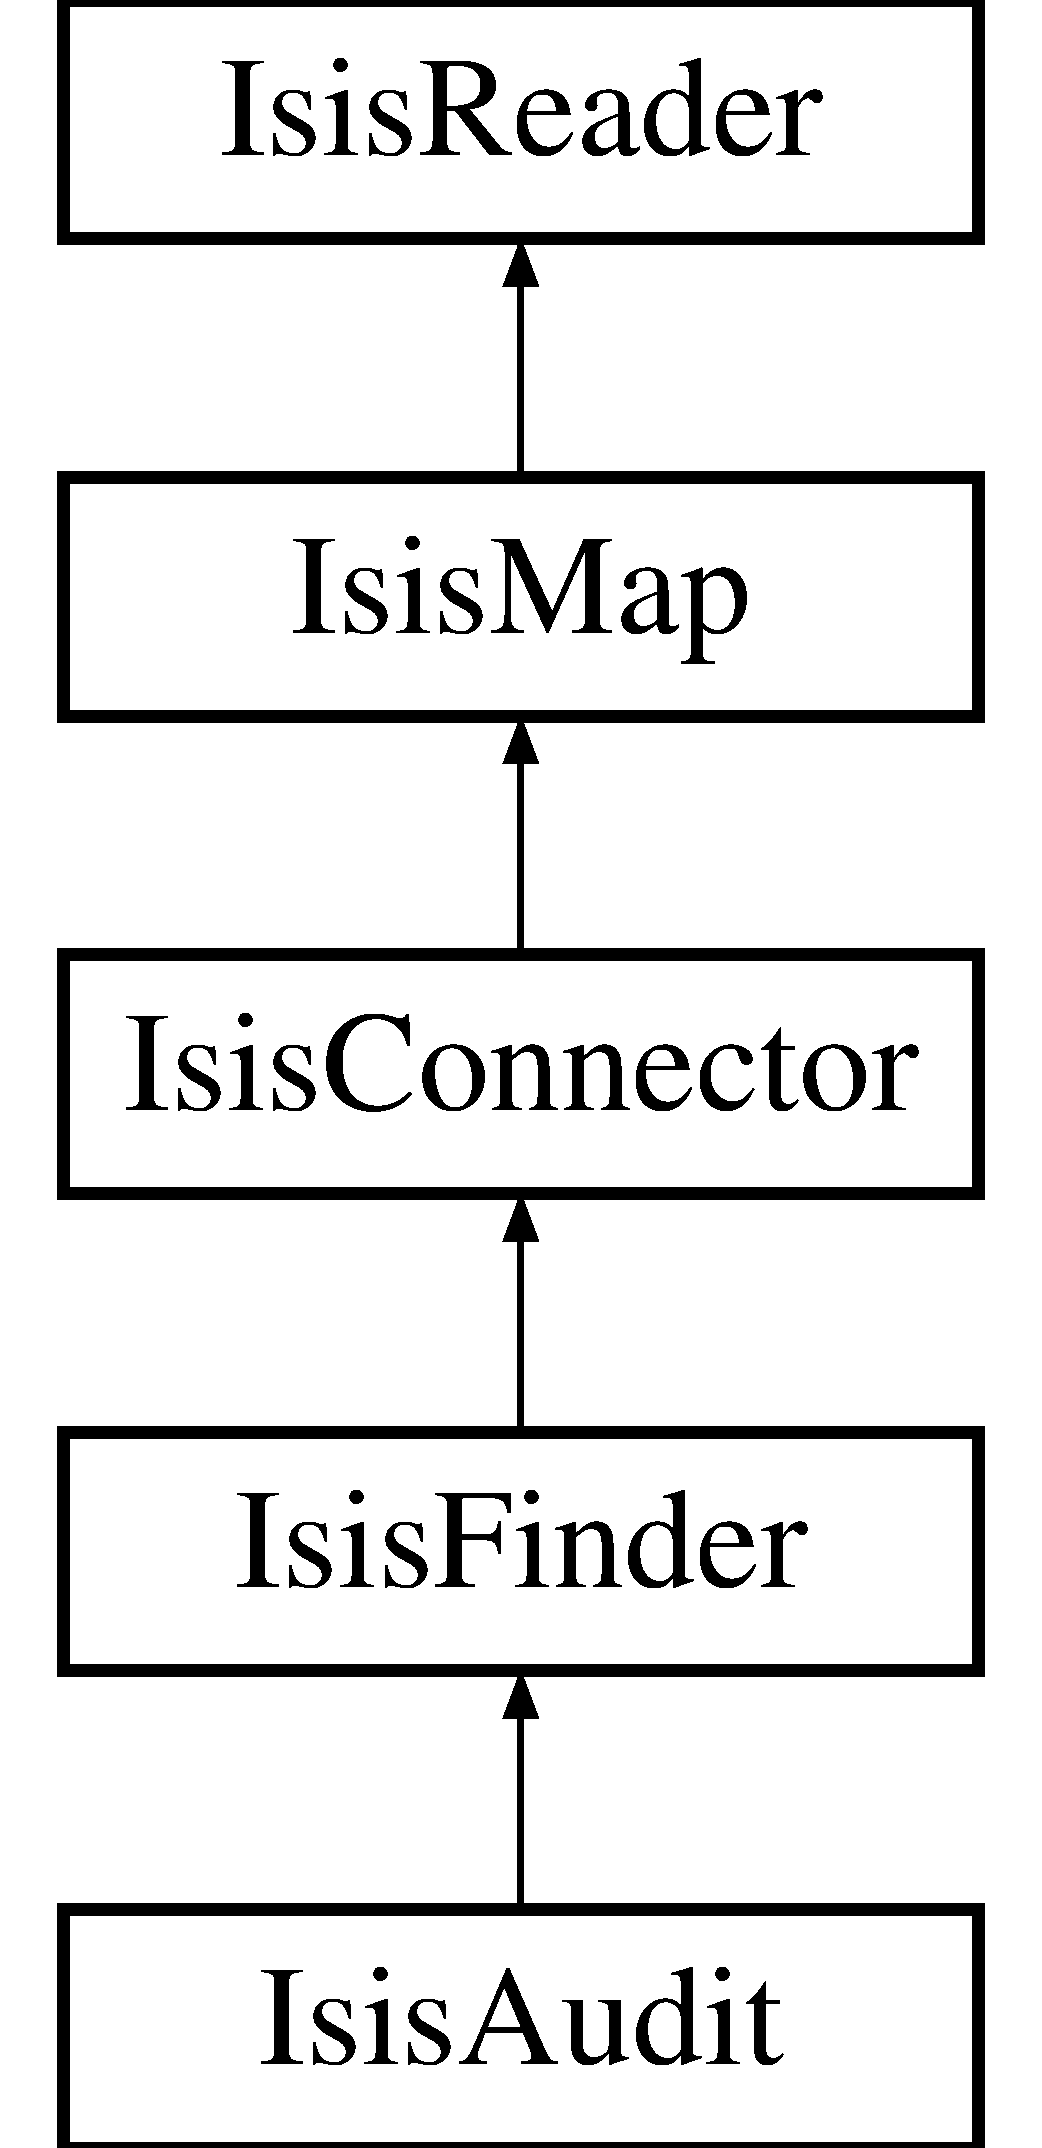
\includegraphics[height=5cm]{classIsisAudit}
\end{center}
\end{figure}
\subsection*{Public Member Functions}
\begin{DoxyCompactItemize}
\item 
\hyperlink{classIsisAudit_a2fb1d5a12933f63f396188bc4229f671}{run} ()
\end{DoxyCompactItemize}


\subsection{Detailed Description}
Methods for auditing an Isis database. 

\subsection{Member Function Documentation}
\hypertarget{classIsisAudit_a2fb1d5a12933f63f396188bc4229f671}{
\index{IsisAudit@{IsisAudit}!run@{run}}
\index{run@{run}!IsisAudit@{IsisAudit}}
\subsubsection[{run}]{\setlength{\rightskip}{0pt plus 5cm}IsisAudit::run ()}}
\label{classIsisAudit_a2fb1d5a12933f63f396188bc4229f671}
Run a standard audit procedure. 

The documentation for this class was generated from the following file:\begin{DoxyCompactItemize}
\item 
classes/IsisAudit.php\end{DoxyCompactItemize}

\hypertarget{classIsisConnector}{
\section{IsisConnector Class Reference}
\label{classIsisConnector}\index{IsisConnector@{IsisConnector}}
}
Inheritance diagram for IsisConnector:\begin{figure}[H]
\begin{center}
\leavevmode
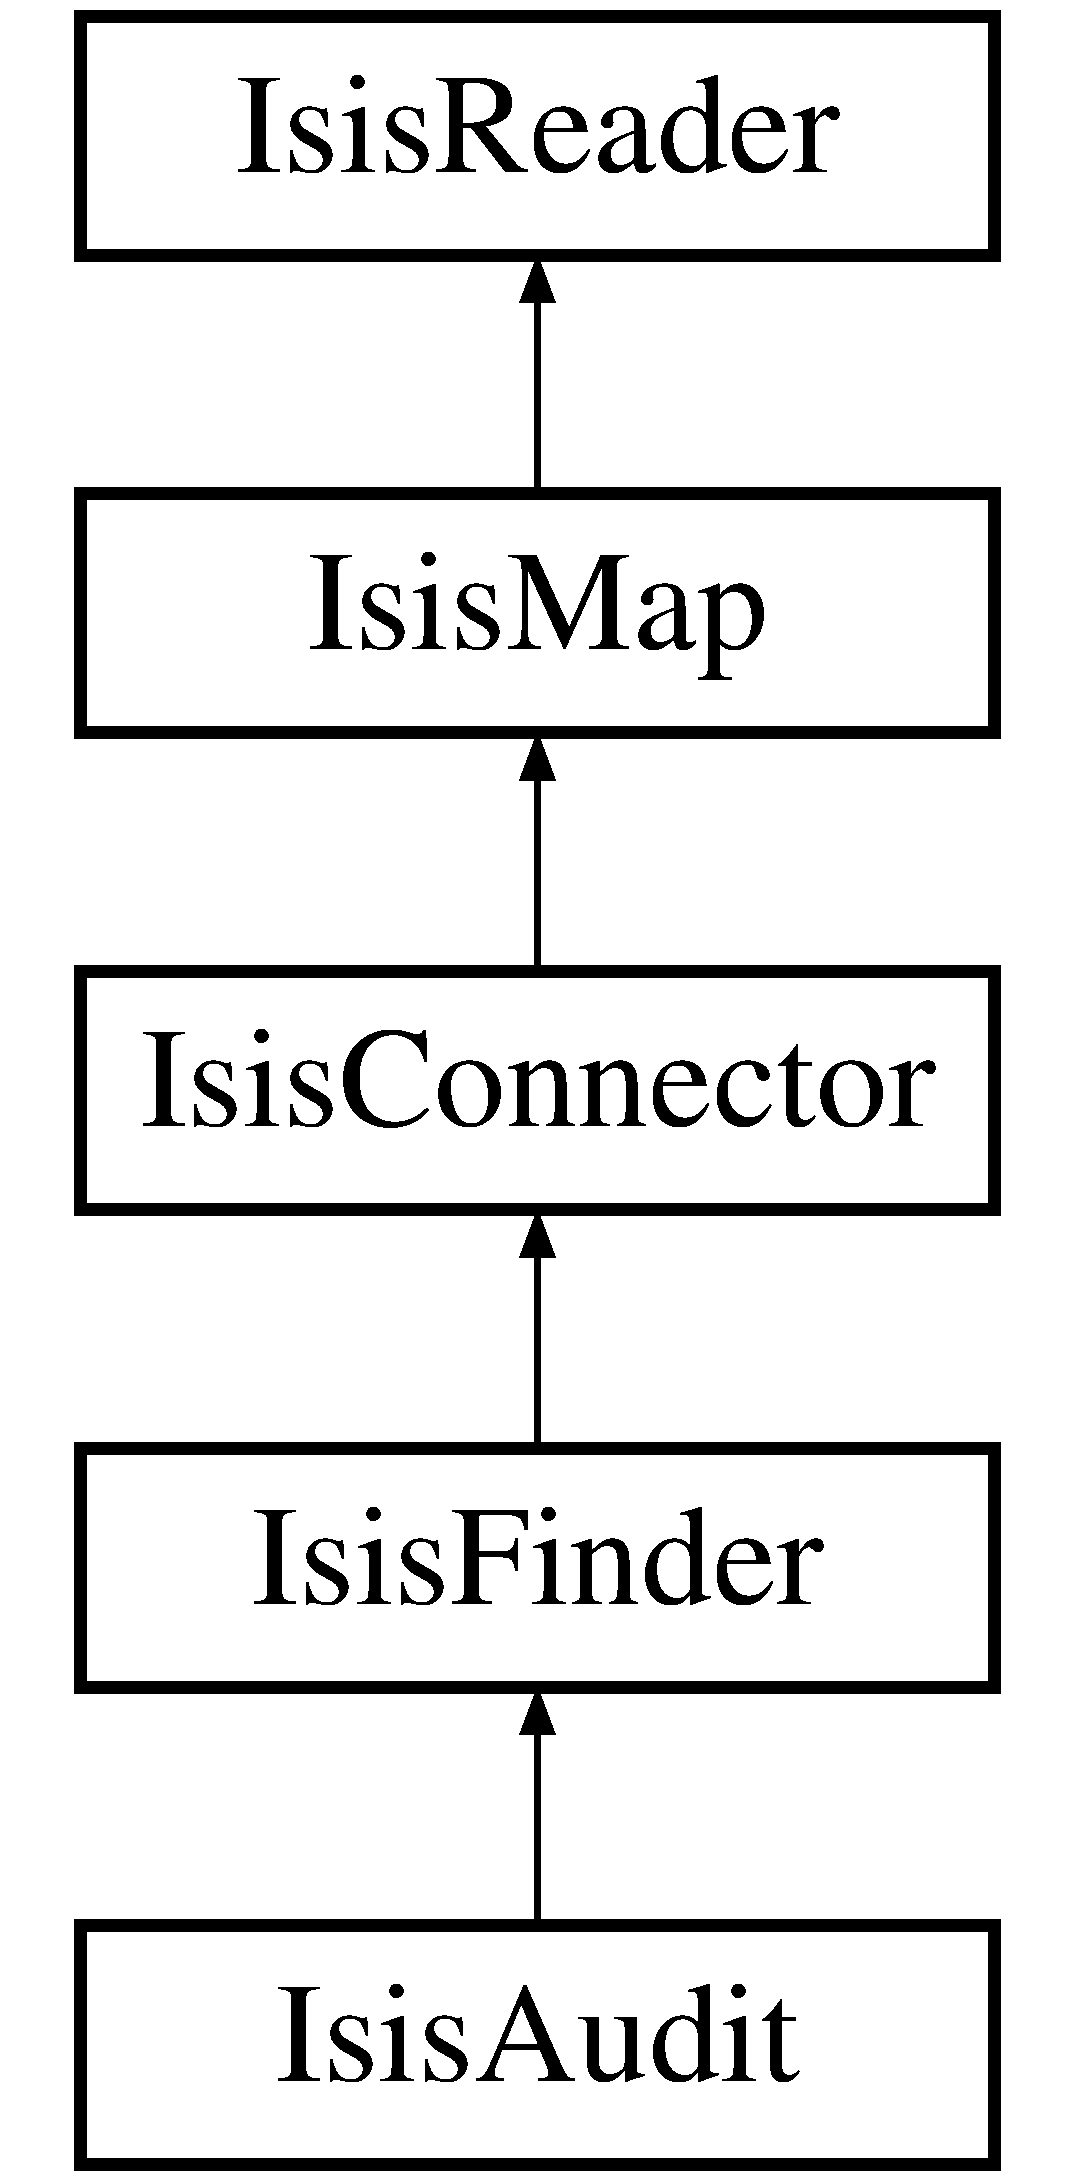
\includegraphics[height=5cm]{classIsisConnector}
\end{center}
\end{figure}
\subsection*{Public Member Functions}
\begin{DoxyCompactItemize}
\item 
\hyperlink{classIsisConnector_a0d1ebc176fe54568044aae02d7932c9b}{getRows} (\$field)
\item 
\hyperlink{classIsisConnector_ad806dcc5be703fe9aea63d72d68af0a2}{getValues} (\$field)
\item 
\hyperlink{classIsisConnector_aa16bb24a54837048eee6244957cbf091}{getItem} (\$field, \$item, \$row=0)
\item 
\hyperlink{classIsisConnector_aa928456a26e0264bf0c1a4869a02cbb3}{getItems} (\$field, \$item)
\item 
\hyperlink{classIsisConnector_a21c7c4e9fec2440f8c7d36f8a632c8c2}{getMainItem} (\$field, \$row=0)
\item 
\hyperlink{classIsisConnector_a2bace7162ec3bf49df9f7acd9367c360}{getMainItems} (\$field)
\item 
\hyperlink{classIsisConnector_a1ddaff24266ee02d652de9a752c1be8e}{getSubfield} (\$field, \$subfield, \$row=0)
\item 
\hyperlink{classIsisConnector_ad8af0f5cef3b139649d9fb317264df10}{getSubfields} (\$field, \$subfield)
\item 
\hyperlink{classIsisConnector_afc97554b42b8b9e98f396811bbfa13d8}{explodeSubfield} (\$field, \$subfield, \$row)
\item 
\hyperlink{classIsisConnector_acfea4d86a683cc7455d258cdb80db478}{explodeItem} (\$field, \$item, \$row)
\item 
\hyperlink{classIsisConnector_a8baad24b6abc2ef29d8968f353ea6dae}{filterSubfield} (\$field, \$subfield, \$row)
\item 
\hyperlink{classIsisConnector_ad88ed9012aac0687aef1c8554879cd52}{hasItem} (\$field, \$item, \$row=0)
\item 
\hyperlink{classIsisConnector_a7bc914f2aa6c523404f368dc0b7b130b}{hasMainItem} (\$field, \$row)
\item 
\hyperlink{classIsisConnector_a2e6970a3aca76a1dbb5b4bb5ac3adda1}{hasSubfield} (\$field, \$subfield, \$row)
\item 
\hyperlink{classIsisConnector_a10669b49c4145a86dc3662c77733d74d}{existingItemKeys} (\$field, \$row=0)
\item 
\hyperlink{classIsisConnector_afbcef48a723b073a2777d5a5ed73d280}{hasFieldSubfieldCondition} (\$field, \$subfield, \$key, \$subkey)
\item 
\hyperlink{classIsisConnector_a9050227e8d8f10821a4df08a5705832a}{specialItem} (\$field, \$subfield, \$return= 'boolean')
\end{DoxyCompactItemize}


\subsection{Detailed Description}
\hyperlink{classIsisConnector}{IsisConnector}: provides an easy interface to connect an application with \hyperlink{classCinisis}{Cinisis}. 

\subsection{Member Function Documentation}
\hypertarget{classIsisConnector_a10669b49c4145a86dc3662c77733d74d}{
\index{IsisConnector@{IsisConnector}!existingItemKeys@{existingItemKeys}}
\index{existingItemKeys@{existingItemKeys}!IsisConnector@{IsisConnector}}
\subsubsection[{existingItemKeys}]{\setlength{\rightskip}{0pt plus 5cm}IsisConnector::existingItemKeys (\$ {\em field}, \/  \$ {\em row} = {\ttfamily 0})}}
\label{classIsisConnector_a10669b49c4145a86dc3662c77733d74d}
Return the existing key items for a result.


\begin{DoxyParams}{Parameters}
\item[{\em \$field}]Field data.\item[{\em \$row}]Row number.\end{DoxyParams}
\begin{DoxyReturn}{Returns}
Array with existing item keys
\end{DoxyReturn}
\begin{Desc}
\item[\hyperlink{todo__todo000001}{Todo}]Test. \end{Desc}
\hypertarget{classIsisConnector_acfea4d86a683cc7455d258cdb80db478}{
\index{IsisConnector@{IsisConnector}!explodeItem@{explodeItem}}
\index{explodeItem@{explodeItem}!IsisConnector@{IsisConnector}}
\subsubsection[{explodeItem}]{\setlength{\rightskip}{0pt plus 5cm}IsisConnector::explodeItem (\$ {\em field}, \/  \$ {\em item}, \/  \$ {\em row})}}
\label{classIsisConnector_acfea4d86a683cc7455d258cdb80db478}
Explode brackets for a given item, avoiding null entries.


\begin{DoxyParams}{Parameters}
\item[{\em \$field}]Field data.\item[{\em \$item}]Item.\item[{\em \$row}]Row number.\end{DoxyParams}
\begin{DoxyReturn}{Returns}
Exploded item data. 
\end{DoxyReturn}
\hypertarget{classIsisConnector_afc97554b42b8b9e98f396811bbfa13d8}{
\index{IsisConnector@{IsisConnector}!explodeSubfield@{explodeSubfield}}
\index{explodeSubfield@{explodeSubfield}!IsisConnector@{IsisConnector}}
\subsubsection[{explodeSubfield}]{\setlength{\rightskip}{0pt plus 5cm}IsisConnector::explodeSubfield (\$ {\em field}, \/  \$ {\em subfield}, \/  \$ {\em row})}}
\label{classIsisConnector_afc97554b42b8b9e98f396811bbfa13d8}
Explode brackets for a given subfield, avoiding null entries.


\begin{DoxyParams}{Parameters}
\item[{\em \$field}]Field data.\item[{\em \$subfield}]Subfield.\item[{\em \$row}]Row number.\end{DoxyParams}
\begin{DoxyReturn}{Returns}
Exploded subfield data. 
\end{DoxyReturn}
\hypertarget{classIsisConnector_a8baad24b6abc2ef29d8968f353ea6dae}{
\index{IsisConnector@{IsisConnector}!filterSubfield@{filterSubfield}}
\index{filterSubfield@{filterSubfield}!IsisConnector@{IsisConnector}}
\subsubsection[{filterSubfield}]{\setlength{\rightskip}{0pt plus 5cm}IsisConnector::filterSubfield (\$ {\em field}, \/  \$ {\em subfield}, \/  \$ {\em row})}}
\label{classIsisConnector_a8baad24b6abc2ef29d8968f353ea6dae}
Filter brackets for a given subfield.


\begin{DoxyParams}{Parameters}
\item[{\em \$field}]Field data.\item[{\em \$subfield}]Subfield.\item[{\em \$row}]Row number.\end{DoxyParams}
\begin{DoxyReturn}{Returns}
Filterd subfield data. 
\end{DoxyReturn}
\hypertarget{classIsisConnector_aa16bb24a54837048eee6244957cbf091}{
\index{IsisConnector@{IsisConnector}!getItem@{getItem}}
\index{getItem@{getItem}!IsisConnector@{IsisConnector}}
\subsubsection[{getItem}]{\setlength{\rightskip}{0pt plus 5cm}IsisConnector::getItem (\$ {\em field}, \/  \$ {\em item}, \/  \$ {\em row} = {\ttfamily 0})}}
\label{classIsisConnector_aa16bb24a54837048eee6244957cbf091}
Get both main field or subfields from a given field and row.


\begin{DoxyParams}{Parameters}
\item[{\em \$field}]field array.\item[{\em \$item}]item name (field or subfield).\item[{\em \$row}]row number.\end{DoxyParams}
\begin{DoxyReturn}{Returns}
Item data. 
\end{DoxyReturn}
\hypertarget{classIsisConnector_aa928456a26e0264bf0c1a4869a02cbb3}{
\index{IsisConnector@{IsisConnector}!getItems@{getItems}}
\index{getItems@{getItems}!IsisConnector@{IsisConnector}}
\subsubsection[{getItems}]{\setlength{\rightskip}{0pt plus 5cm}IsisConnector::getItems (\$ {\em field}, \/  \$ {\em item})}}
\label{classIsisConnector_aa928456a26e0264bf0c1a4869a02cbb3}
Get all rows both main field or subfields from a given field.


\begin{DoxyParams}{Parameters}
\item[{\em \$field}]field array.\item[{\em \$item}]item name (field or subfield).\end{DoxyParams}
\begin{DoxyReturn}{Returns}
Item data. 
\end{DoxyReturn}
\hypertarget{classIsisConnector_a21c7c4e9fec2440f8c7d36f8a632c8c2}{
\index{IsisConnector@{IsisConnector}!getMainItem@{getMainItem}}
\index{getMainItem@{getMainItem}!IsisConnector@{IsisConnector}}
\subsubsection[{getMainItem}]{\setlength{\rightskip}{0pt plus 5cm}IsisConnector::getMainItem (\$ {\em field}, \/  \$ {\em row} = {\ttfamily 0})}}
\label{classIsisConnector_a21c7c4e9fec2440f8c7d36f8a632c8c2}
Get the value of a given field.


\begin{DoxyParams}{Parameters}
\item[{\em \$field}]Field array.\item[{\em \$row}]Optional row number if repetitive field.\end{DoxyParams}
\begin{DoxyReturn}{Returns}
Field data. 
\end{DoxyReturn}
\hypertarget{classIsisConnector_a2bace7162ec3bf49df9f7acd9367c360}{
\index{IsisConnector@{IsisConnector}!getMainItems@{getMainItems}}
\index{getMainItems@{getMainItems}!IsisConnector@{IsisConnector}}
\subsubsection[{getMainItems}]{\setlength{\rightskip}{0pt plus 5cm}IsisConnector::getMainItems (\$ {\em field})}}
\label{classIsisConnector_a2bace7162ec3bf49df9f7acd9367c360}
Get all values of a given field.


\begin{DoxyParams}{Parameters}
\item[{\em \$field}]Field array.\end{DoxyParams}
\begin{DoxyReturn}{Returns}
Field data. 
\end{DoxyReturn}
\hypertarget{classIsisConnector_a0d1ebc176fe54568044aae02d7932c9b}{
\index{IsisConnector@{IsisConnector}!getRows@{getRows}}
\index{getRows@{getRows}!IsisConnector@{IsisConnector}}
\subsubsection[{getRows}]{\setlength{\rightskip}{0pt plus 5cm}IsisConnector::getRows (\$ {\em field})}}
\label{classIsisConnector_a0d1ebc176fe54568044aae02d7932c9b}
Get the number of resulting rows for a given field.


\begin{DoxyParams}{Parameters}
\item[{\em \$field}]Field array.\end{DoxyParams}
\begin{DoxyReturn}{Returns}
Number of rows. 
\end{DoxyReturn}
\hypertarget{classIsisConnector_a1ddaff24266ee02d652de9a752c1be8e}{
\index{IsisConnector@{IsisConnector}!getSubfield@{getSubfield}}
\index{getSubfield@{getSubfield}!IsisConnector@{IsisConnector}}
\subsubsection[{getSubfield}]{\setlength{\rightskip}{0pt plus 5cm}IsisConnector::getSubfield (\$ {\em field}, \/  \$ {\em subfield}, \/  \$ {\em row} = {\ttfamily 0})}}
\label{classIsisConnector_a1ddaff24266ee02d652de9a752c1be8e}
Get the value of a given subfield.


\begin{DoxyParams}{Parameters}
\item[{\em \$field}]Field array.\item[{\em \$subfield}]Subfield name.\item[{\em \$row}]Row number if repetitive data.\end{DoxyParams}
\begin{DoxyReturn}{Returns}
Subfield data. 
\end{DoxyReturn}
\hypertarget{classIsisConnector_ad8af0f5cef3b139649d9fb317264df10}{
\index{IsisConnector@{IsisConnector}!getSubfields@{getSubfields}}
\index{getSubfields@{getSubfields}!IsisConnector@{IsisConnector}}
\subsubsection[{getSubfields}]{\setlength{\rightskip}{0pt plus 5cm}IsisConnector::getSubfields (\$ {\em field}, \/  \$ {\em subfield})}}
\label{classIsisConnector_ad8af0f5cef3b139649d9fb317264df10}
Get all values of a given subfield.


\begin{DoxyParams}{Parameters}
\item[{\em \$field}]Field array.\item[{\em \$subfield}]Subfield name.\end{DoxyParams}
\begin{DoxyReturn}{Returns}
Subfield data. 
\end{DoxyReturn}
\hypertarget{classIsisConnector_ad806dcc5be703fe9aea63d72d68af0a2}{
\index{IsisConnector@{IsisConnector}!getValues@{getValues}}
\index{getValues@{getValues}!IsisConnector@{IsisConnector}}
\subsubsection[{getValues}]{\setlength{\rightskip}{0pt plus 5cm}IsisConnector::getValues (\$ {\em field})}}
\label{classIsisConnector_ad806dcc5be703fe9aea63d72d68af0a2}
Get all values of a given field.


\begin{DoxyParams}{Parameters}
\item[{\em \$field}]Field array.\end{DoxyParams}
\begin{DoxyReturn}{Returns}
Field data. 
\end{DoxyReturn}
\hypertarget{classIsisConnector_afbcef48a723b073a2777d5a5ed73d280}{
\index{IsisConnector@{IsisConnector}!hasFieldSubfieldCondition@{hasFieldSubfieldCondition}}
\index{hasFieldSubfieldCondition@{hasFieldSubfieldCondition}!IsisConnector@{IsisConnector}}
\subsubsection[{hasFieldSubfieldCondition}]{\setlength{\rightskip}{0pt plus 5cm}IsisConnector::hasFieldSubfieldCondition (\$ {\em field}, \/  \$ {\em subfield}, \/  \$ {\em key}, \/  \$ {\em subkey})}}
\label{classIsisConnector_afbcef48a723b073a2777d5a5ed73d280}
Check if a field and subfield match a given condition.


\begin{DoxyParams}{Parameters}
\item[{\em \$field}]Field data.\item[{\em \$subfield}]Subfield.\item[{\em \$key}]Field key.\item[{\em \$subkey}]Subfield key.\end{DoxyParams}
\begin{DoxyReturn}{Returns}
True if condition match, false otherwise. 
\end{DoxyReturn}
\hypertarget{classIsisConnector_ad88ed9012aac0687aef1c8554879cd52}{
\index{IsisConnector@{IsisConnector}!hasItem@{hasItem}}
\index{hasItem@{hasItem}!IsisConnector@{IsisConnector}}
\subsubsection[{hasItem}]{\setlength{\rightskip}{0pt plus 5cm}IsisConnector::hasItem (\$ {\em field}, \/  \$ {\em item}, \/  \$ {\em row} = {\ttfamily 0})}}
\label{classIsisConnector_ad88ed9012aac0687aef1c8554879cd52}
Check if a field result has an item.


\begin{DoxyParams}{Parameters}
\item[{\em \$field}]Field data.\item[{\em \$item}]Item code ('main' for the main item).\item[{\em \$row}]Row number.\end{DoxyParams}
\begin{DoxyReturn}{Returns}
True if result has the main item, false otherwise. 
\end{DoxyReturn}
\hypertarget{classIsisConnector_a7bc914f2aa6c523404f368dc0b7b130b}{
\index{IsisConnector@{IsisConnector}!hasMainItem@{hasMainItem}}
\index{hasMainItem@{hasMainItem}!IsisConnector@{IsisConnector}}
\subsubsection[{hasMainItem}]{\setlength{\rightskip}{0pt plus 5cm}IsisConnector::hasMainItem (\$ {\em field}, \/  \$ {\em row})}}
\label{classIsisConnector_a7bc914f2aa6c523404f368dc0b7b130b}
Check if a field result has a main item.


\begin{DoxyParams}{Parameters}
\item[{\em \$field}]Field data.\item[{\em \$row}]Row number.\end{DoxyParams}
\begin{DoxyReturn}{Returns}
True if result has the main item, false otherwise. 
\end{DoxyReturn}
\hypertarget{classIsisConnector_a2e6970a3aca76a1dbb5b4bb5ac3adda1}{
\index{IsisConnector@{IsisConnector}!hasSubfield@{hasSubfield}}
\index{hasSubfield@{hasSubfield}!IsisConnector@{IsisConnector}}
\subsubsection[{hasSubfield}]{\setlength{\rightskip}{0pt plus 5cm}IsisConnector::hasSubfield (\$ {\em field}, \/  \$ {\em subfield}, \/  \$ {\em row})}}
\label{classIsisConnector_a2e6970a3aca76a1dbb5b4bb5ac3adda1}
Check if a field result and row has a given subfield.


\begin{DoxyParams}{Parameters}
\item[{\em \$field}]Field data.\item[{\em \$subfield}]Subfield.\item[{\em \$row}]Row number.\end{DoxyParams}
\begin{DoxyReturn}{Returns}
True if result has the subfield, false otherwise. 
\end{DoxyReturn}
\hypertarget{classIsisConnector_a9050227e8d8f10821a4df08a5705832a}{
\index{IsisConnector@{IsisConnector}!specialItem@{specialItem}}
\index{specialItem@{specialItem}!IsisConnector@{IsisConnector}}
\subsubsection[{specialItem}]{\setlength{\rightskip}{0pt plus 5cm}IsisConnector::specialItem (\$ {\em field}, \/  \$ {\em subfield}, \/  \$ {\em return} = {\ttfamily 'boolean'})}}
\label{classIsisConnector_a9050227e8d8f10821a4df08a5705832a}
Deal with special items.


\begin{DoxyParams}{Parameters}
\item[{\em \$field}]Field data from ISIS database schema.\item[{\em \$subfield}]Subfield name.\item[{\em \$return}]Specify return type.\end{DoxyParams}
\begin{DoxyReturn}{Returns}
True if special subfield, false otherwise of special return type 
\end{DoxyReturn}


The documentation for this class was generated from the following file:\begin{DoxyCompactItemize}
\item 
classes/IsisConnector.php\end{DoxyCompactItemize}

\hypertarget{interfaceIsisDb}{
\section{IsisDb Interface Reference}
\label{interfaceIsisDb}\index{IsisDb@{IsisDb}}
}
Inheritance diagram for IsisDb:\begin{figure}[H]
\begin{center}
\leavevmode
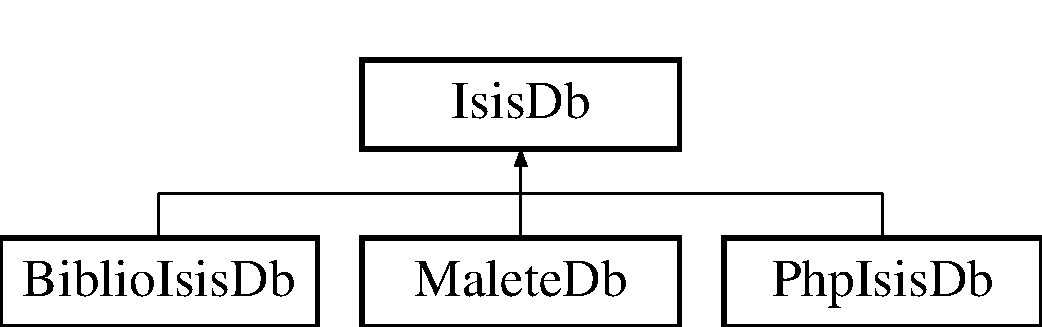
\includegraphics[height=2cm]{interfaceIsisDb}
\end{center}
\end{figure}
\subsection*{Public Member Functions}
\begin{DoxyCompactItemize}
\item 
\hyperlink{interfaceIsisDb_ae1c0a3496d55f710d34c5c19ada7a66b}{\_\-\_\-construct} (\$schema)
\item 
\hyperlink{interfaceIsisDb_a68335ec0db01ef03f0725621b38b5686}{read} (\$id)
\item 
\hyperlink{interfaceIsisDb_a86f38eca2b6d0835b60770d8a4e511ff}{entries} ()
\item 
\hyperlink{interfaceIsisDb_a857c10d90da64067efa17afb2f32edb6}{example} ()
\end{DoxyCompactItemize}
\subsection*{Static Public Member Functions}
\begin{DoxyCompactItemize}
\item 
static \hyperlink{interfaceIsisDb_af681b8f990b579f1835aa7ba4c83f1b8}{check} (\$schema, \$section=NULL)
\end{DoxyCompactItemize}


\subsection{Detailed Description}
Generic interface for reading Isis databases. 

\subsection{Constructor \& Destructor Documentation}
\hypertarget{interfaceIsisDb_ae1c0a3496d55f710d34c5c19ada7a66b}{
\index{IsisDb@{IsisDb}!\_\-\_\-construct@{\_\-\_\-construct}}
\index{\_\-\_\-construct@{\_\-\_\-construct}!IsisDb@{IsisDb}}
\subsubsection[{\_\-\_\-construct}]{\setlength{\rightskip}{0pt plus 5cm}IsisDb::\_\-\_\-construct (\$ {\em schema})}}
\label{interfaceIsisDb_ae1c0a3496d55f710d34c5c19ada7a66b}
Constructor.

The implementation constructor should accept a database schema definition and setup the appropriate db resource.


\begin{DoxyParams}{Parameters}
\item[{\em \$schema}]High level database schema description.\end{DoxyParams}
\begin{DoxyReturn}{Returns}
Database resource or FALSE in case of error.
\end{DoxyReturn}
\begin{DoxySeeAlso}{See also}
default\_\-schema() 
\end{DoxySeeAlso}


Implemented in \hyperlink{classBiblioIsisDb_ab2c5ec782b324847e104d8ad35a230af}{BiblioIsisDb}, \hyperlink{classMaleteDb_a60f87371bc1ec156b010e5b38b4c22e2}{MaleteDb}, and \hyperlink{classPhpIsisDb_abb6db51373d065baf9135fd278653bc5}{PhpIsisDb}.



\subsection{Member Function Documentation}
\hypertarget{interfaceIsisDb_af681b8f990b579f1835aa7ba4c83f1b8}{
\index{IsisDb@{IsisDb}!check@{check}}
\index{check@{check}!IsisDb@{IsisDb}}
\subsubsection[{check}]{\setlength{\rightskip}{0pt plus 5cm}static IsisDb::check (\$ {\em schema}, \/  \$ {\em section} = {\ttfamily NULL})\hspace{0.3cm}{\ttfamily  \mbox{[}static\mbox{]}}}}
\label{interfaceIsisDb_af681b8f990b579f1835aa7ba4c83f1b8}
Configuration check.


\begin{DoxyParams}{Parameters}
\item[{\em \$schema}]Database schema to check.\item[{\em \$section}]Configuration section.\end{DoxyParams}
\begin{DoxyReturn}{Returns}
Database schema or FALSE if error. 
\end{DoxyReturn}


Implemented in \hyperlink{classBiblioIsisDb_a929467f1907d3aeaeebe493f0c188c5b}{BiblioIsisDb}, \hyperlink{classMaleteDb_ab2da32d84af17df79d947ae32257b4ec}{MaleteDb}, and \hyperlink{classPhpIsisDb_a23761cc04114090a2863467b2accc80a}{PhpIsisDb}.

\hypertarget{interfaceIsisDb_a86f38eca2b6d0835b60770d8a4e511ff}{
\index{IsisDb@{IsisDb}!entries@{entries}}
\index{entries@{entries}!IsisDb@{IsisDb}}
\subsubsection[{entries}]{\setlength{\rightskip}{0pt plus 5cm}IsisDb::entries ()}}
\label{interfaceIsisDb_a86f38eca2b6d0835b60770d8a4e511ff}
Return number of entries in the database.

\begin{DoxyReturn}{Returns}
Number of entries in the database. 
\end{DoxyReturn}


Implemented in \hyperlink{classBiblioIsisDb_ab6b0a977c066c25c6bdca5c1d3a083e8}{BiblioIsisDb}, \hyperlink{classMaleteDb_a5c6cb09a072e5d2ddce31c77098ccba4}{MaleteDb}, and \hyperlink{classPhpIsisDb_a0491ce84e5a85e775f811f18e63ef0fb}{PhpIsisDb}.

\hypertarget{interfaceIsisDb_a857c10d90da64067efa17afb2f32edb6}{
\index{IsisDb@{IsisDb}!example@{example}}
\index{example@{example}!IsisDb@{IsisDb}}
\subsubsection[{example}]{\setlength{\rightskip}{0pt plus 5cm}IsisDb::example ()}}
\label{interfaceIsisDb_a857c10d90da64067efa17afb2f32edb6}
Return an example database schema.

The example schema should have all information the implementation needs to be able to open and read a database.

\begin{DoxyReturn}{Returns}
Array with a sample database schema. 
\end{DoxyReturn}


Implemented in \hyperlink{classBiblioIsisDb_a8e76b289b9e3a9893b9469094753d2bc}{BiblioIsisDb}, \hyperlink{classMaleteDb_a4f16c48facae498d0db1a042e9727d04}{MaleteDb}, and \hyperlink{classPhpIsisDb_a7f4f3a9fd6dab86bd3cb3149d65f92cd}{PhpIsisDb}.

\hypertarget{interfaceIsisDb_a68335ec0db01ef03f0725621b38b5686}{
\index{IsisDb@{IsisDb}!read@{read}}
\index{read@{read}!IsisDb@{IsisDb}}
\subsubsection[{read}]{\setlength{\rightskip}{0pt plus 5cm}IsisDb::read (\$ {\em id})}}
\label{interfaceIsisDb_a68335ec0db01ef03f0725621b38b5686}
Read an entry from the database.


\begin{DoxyParams}{Parameters}
\item[{\em \$id}]Database entry id. \end{DoxyParams}


Implemented in \hyperlink{classMaleteDb_ad2a65876db24adc388afce465e0c153e}{MaleteDb}, and \hyperlink{classPhpIsisDb_af2266931746f6f2335b831be8b8333fb}{PhpIsisDb}.



The documentation for this interface was generated from the following file:\begin{DoxyCompactItemize}
\item 
classes/backends/IsisDb.php\end{DoxyCompactItemize}

\hypertarget{classIsisEntryIterator}{
\section{IsisEntryIterator Class Reference}
\label{classIsisEntryIterator}\index{IsisEntryIterator@{IsisEntryIterator}}
}
\subsection*{Public Member Functions}
\begin{DoxyCompactItemize}
\item 
\hyperlink{classIsisEntryIterator_a056fcc7d817523faf1fb033fa9f8ad6e}{\_\-\_\-construct} (\$class, \$entry=1)
\item 
\hyperlink{classIsisEntryIterator_a985e88cdfb69b42e3389f24c08b2404a}{rewind} ()
\item 
\hyperlink{classIsisEntryIterator_a4a740dacedb86023ece4561092c33a65}{key} ()
\item 
\hyperlink{classIsisEntryIterator_ac482f43403fc4d2e1b620fb4e0f6797f}{current} ()
\item 
\hyperlink{classIsisEntryIterator_a2d1d0fe5d3c22d1720e93e03952b877d}{next} ()
\item 
\hyperlink{classIsisEntryIterator_aff9e54b112cc728b7cd6cf00c0359c49}{valid} ()
\end{DoxyCompactItemize}


\subsection{Detailed Description}
Isis entry iterator. Iterates over all entries in the database. 

\subsection{Constructor \& Destructor Documentation}
\hypertarget{classIsisEntryIterator_a056fcc7d817523faf1fb033fa9f8ad6e}{
\index{IsisEntryIterator@{IsisEntryIterator}!\_\-\_\-construct@{\_\-\_\-construct}}
\index{\_\-\_\-construct@{\_\-\_\-construct}!IsisEntryIterator@{IsisEntryIterator}}
\subsubsection[{\_\-\_\-construct}]{\setlength{\rightskip}{0pt plus 5cm}IsisEntryIterator::\_\-\_\-construct (
\begin{DoxyParamCaption}
\item[{\$}]{ class, }
\item[{\$}]{ entry = {\ttfamily 1}}
\end{DoxyParamCaption}
)}}
\label{classIsisEntryIterator_a056fcc7d817523faf1fb033fa9f8ad6e}
Constructor.


\begin{DoxyParams}{Parameters}
\item[{\em \$class}]Instance of \hyperlink{classIsisConnector}{IsisConnector} or child class.\item[{\em \$entry}]Start entry number to iterate from. \end{DoxyParams}


\subsection{Member Function Documentation}
\hypertarget{classIsisEntryIterator_ac482f43403fc4d2e1b620fb4e0f6797f}{
\index{IsisEntryIterator@{IsisEntryIterator}!current@{current}}
\index{current@{current}!IsisEntryIterator@{IsisEntryIterator}}
\subsubsection[{current}]{\setlength{\rightskip}{0pt plus 5cm}IsisEntryIterator::current (
\begin{DoxyParamCaption}
{}
\end{DoxyParamCaption}
)}}
\label{classIsisEntryIterator_ac482f43403fc4d2e1b620fb4e0f6797f}
Return the current element. \hypertarget{classIsisEntryIterator_a4a740dacedb86023ece4561092c33a65}{
\index{IsisEntryIterator@{IsisEntryIterator}!key@{key}}
\index{key@{key}!IsisEntryIterator@{IsisEntryIterator}}
\subsubsection[{key}]{\setlength{\rightskip}{0pt plus 5cm}IsisEntryIterator::key (
\begin{DoxyParamCaption}
{}
\end{DoxyParamCaption}
)}}
\label{classIsisEntryIterator_a4a740dacedb86023ece4561092c33a65}
Return the key of the current element. \hypertarget{classIsisEntryIterator_a2d1d0fe5d3c22d1720e93e03952b877d}{
\index{IsisEntryIterator@{IsisEntryIterator}!next@{next}}
\index{next@{next}!IsisEntryIterator@{IsisEntryIterator}}
\subsubsection[{next}]{\setlength{\rightskip}{0pt plus 5cm}IsisEntryIterator::next (
\begin{DoxyParamCaption}
{}
\end{DoxyParamCaption}
)}}
\label{classIsisEntryIterator_a2d1d0fe5d3c22d1720e93e03952b877d}
Move forward to next element. \hypertarget{classIsisEntryIterator_a985e88cdfb69b42e3389f24c08b2404a}{
\index{IsisEntryIterator@{IsisEntryIterator}!rewind@{rewind}}
\index{rewind@{rewind}!IsisEntryIterator@{IsisEntryIterator}}
\subsubsection[{rewind}]{\setlength{\rightskip}{0pt plus 5cm}IsisEntryIterator::rewind (
\begin{DoxyParamCaption}
{}
\end{DoxyParamCaption}
)}}
\label{classIsisEntryIterator_a985e88cdfb69b42e3389f24c08b2404a}
Rewind the Iterator to the first element. \hypertarget{classIsisEntryIterator_aff9e54b112cc728b7cd6cf00c0359c49}{
\index{IsisEntryIterator@{IsisEntryIterator}!valid@{valid}}
\index{valid@{valid}!IsisEntryIterator@{IsisEntryIterator}}
\subsubsection[{valid}]{\setlength{\rightskip}{0pt plus 5cm}IsisEntryIterator::valid (
\begin{DoxyParamCaption}
{}
\end{DoxyParamCaption}
)}}
\label{classIsisEntryIterator_aff9e54b112cc728b7cd6cf00c0359c49}
Check if there is a current element after calls to \hyperlink{classIsisEntryIterator_a985e88cdfb69b42e3389f24c08b2404a}{rewind()} or \hyperlink{classIsisEntryIterator_a2d1d0fe5d3c22d1720e93e03952b877d}{next()}. 

The documentation for this class was generated from the following file:\begin{DoxyCompactItemize}
\item 
classes/iterators/IsisEntryIterator.php\end{DoxyCompactItemize}

\hypertarget{classIsisFinder}{
\section{IsisFinder Class Reference}
\label{classIsisFinder}\index{IsisFinder@{IsisFinder}}
}
Inheritance diagram for IsisFinder:\begin{figure}[H]
\begin{center}
\leavevmode
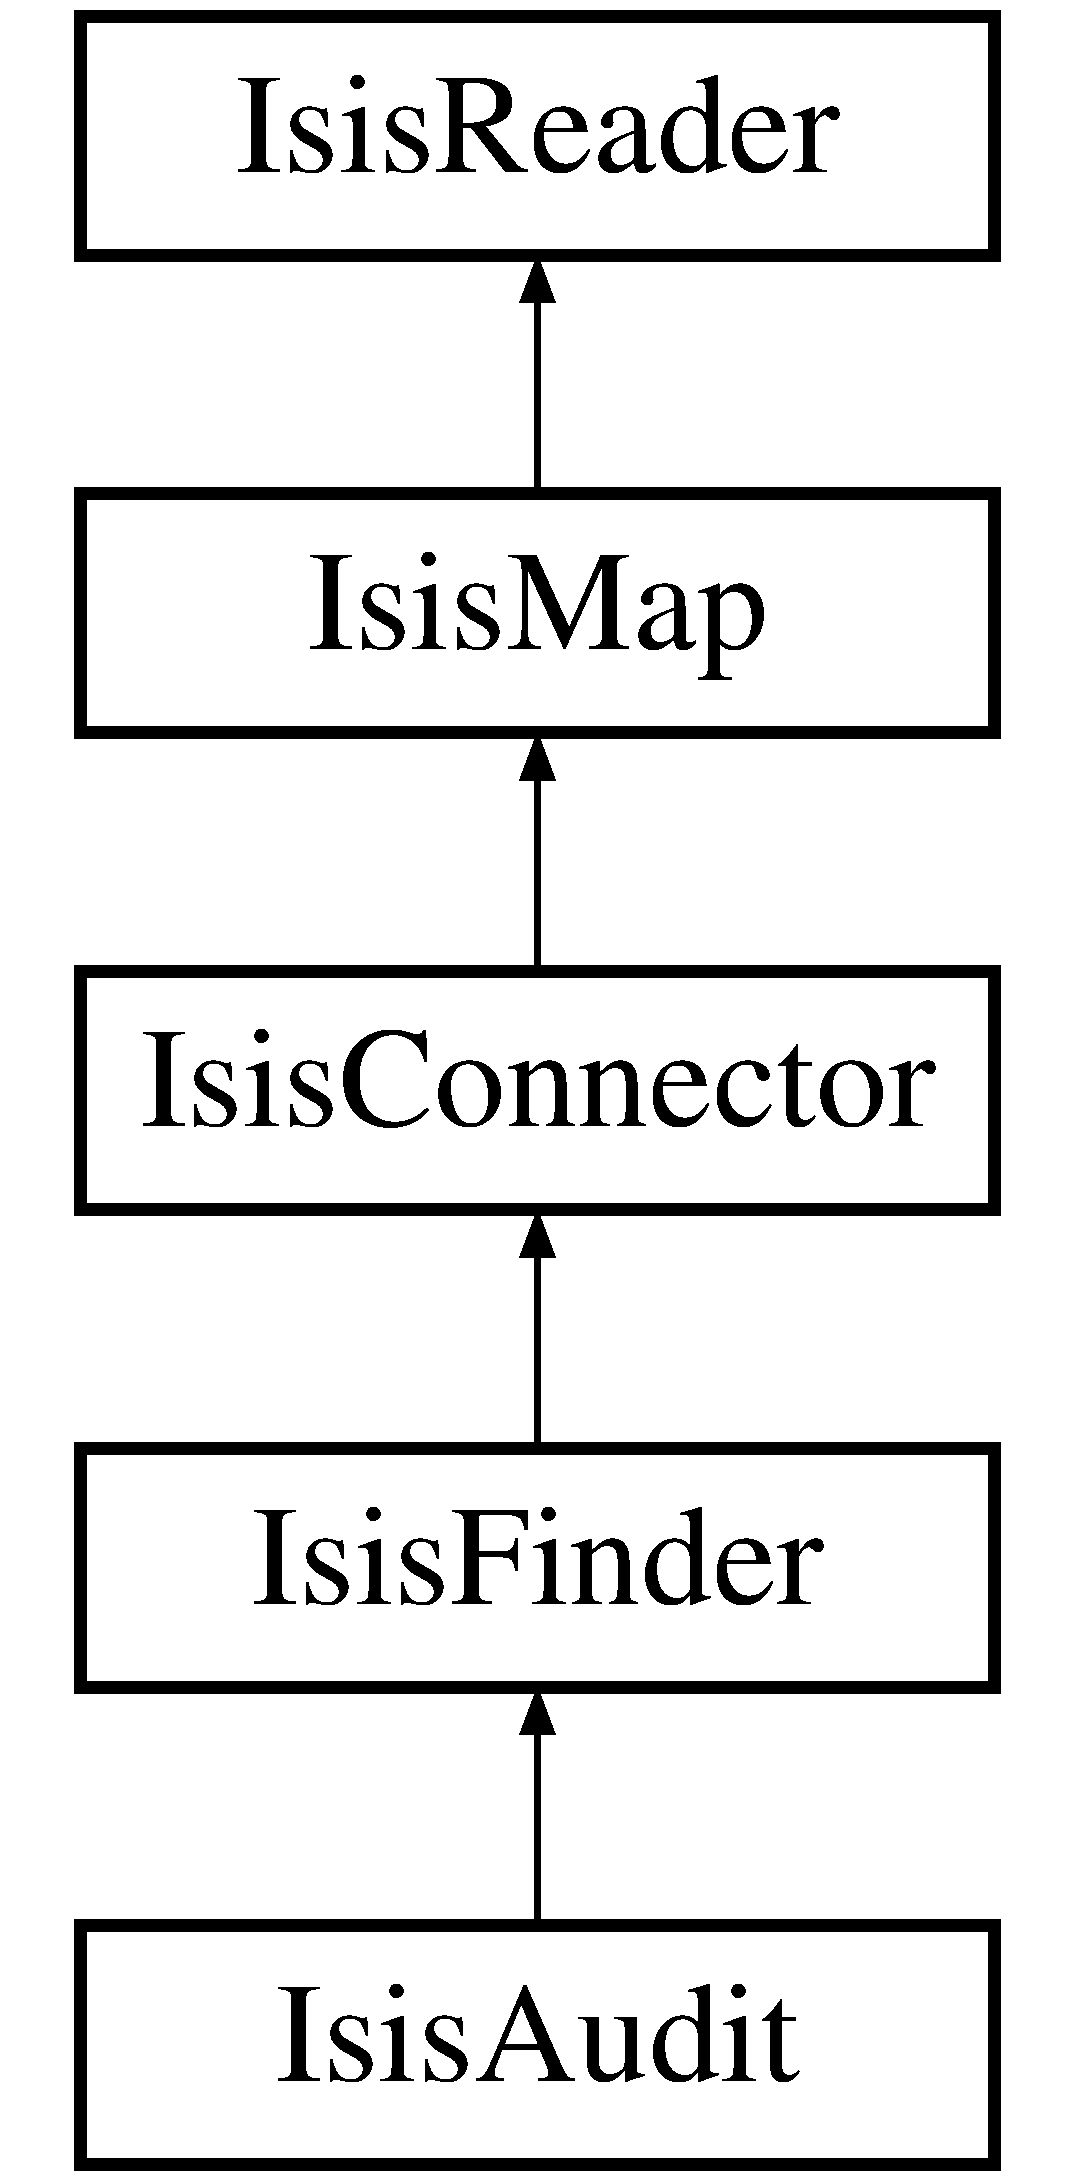
\includegraphics[height=5cm]{classIsisFinder}
\end{center}
\end{figure}
\subsection*{Public Member Functions}
\begin{DoxyCompactItemize}
\item 
\hyperlink{classIsisFinder_ac4e3a8f45995cbf940b3f2899b71bd1e}{nextRepetition} (\$field, \$entry=1)
\item 
\hyperlink{classIsisFinder_a7d708e281bea35ee38f5875c8f2cad8d}{nextField} (\$field, \$entry=1)
\item 
\hyperlink{classIsisFinder_aa367980783d341197e003684a639ff1a}{nextSubfield} (\$field, \$subfield, \$entry=1)
\item 
\hyperlink{classIsisFinder_a41410b18c4462c05ac669e4ee889d8a7}{hasSubfieldInRows} (\$field, \$subfield)
\end{DoxyCompactItemize}


\subsection{Detailed Description}
Provides Isis Database search methods. 

\subsection{Member Function Documentation}
\hypertarget{classIsisFinder_a41410b18c4462c05ac669e4ee889d8a7}{
\index{IsisFinder@{IsisFinder}!hasSubfieldInRows@{hasSubfieldInRows}}
\index{hasSubfieldInRows@{hasSubfieldInRows}!IsisFinder@{IsisFinder}}
\subsubsection[{hasSubfieldInRows}]{\setlength{\rightskip}{0pt plus 5cm}IsisFinder::hasSubfieldInRows (\$ {\em field}, \/  \$ {\em subfield})}}
\label{classIsisFinder_a41410b18c4462c05ac669e4ee889d8a7}
Check if a field result has a given subfield.


\begin{DoxyParams}{Parameters}
\item[{\em \$field}]Field data.\item[{\em \$subfield}]Subfield.\end{DoxyParams}
\begin{DoxyReturn}{Returns}
True if result has the subfield, false otherwise. 
\end{DoxyReturn}
\hypertarget{classIsisFinder_a7d708e281bea35ee38f5875c8f2cad8d}{
\index{IsisFinder@{IsisFinder}!nextField@{nextField}}
\index{nextField@{nextField}!IsisFinder@{IsisFinder}}
\subsubsection[{nextField}]{\setlength{\rightskip}{0pt plus 5cm}IsisFinder::nextField (\$ {\em field}, \/  \$ {\em entry} = {\ttfamily 1})}}
\label{classIsisFinder_a7d708e281bea35ee38f5875c8f2cad8d}
Find the next occurrence of a field.


\begin{DoxyParams}{Parameters}
\item[{\em \$entry}]Start entry number to begin the search.\item[{\em \$field}]Field data.\end{DoxyParams}
\begin{DoxyReturn}{Returns}
Next occurrence. 
\end{DoxyReturn}
\hypertarget{classIsisFinder_ac4e3a8f45995cbf940b3f2899b71bd1e}{
\index{IsisFinder@{IsisFinder}!nextRepetition@{nextRepetition}}
\index{nextRepetition@{nextRepetition}!IsisFinder@{IsisFinder}}
\subsubsection[{nextRepetition}]{\setlength{\rightskip}{0pt plus 5cm}IsisFinder::nextRepetition (\$ {\em field}, \/  \$ {\em entry} = {\ttfamily 1})}}
\label{classIsisFinder_ac4e3a8f45995cbf940b3f2899b71bd1e}
Find the next repetition of a field.


\begin{DoxyParams}{Parameters}
\item[{\em \$entry}]Start entry number to begin the search.\item[{\em \$field}]Field data.\end{DoxyParams}
\begin{DoxyReturn}{Returns}
Next repetition entry and result. 
\end{DoxyReturn}
\hypertarget{classIsisFinder_aa367980783d341197e003684a639ff1a}{
\index{IsisFinder@{IsisFinder}!nextSubfield@{nextSubfield}}
\index{nextSubfield@{nextSubfield}!IsisFinder@{IsisFinder}}
\subsubsection[{nextSubfield}]{\setlength{\rightskip}{0pt plus 5cm}IsisFinder::nextSubfield (\$ {\em field}, \/  \$ {\em subfield}, \/  \$ {\em entry} = {\ttfamily 1})}}
\label{classIsisFinder_aa367980783d341197e003684a639ff1a}
Find the next occurrence of a subfield.


\begin{DoxyParams}{Parameters}
\item[{\em \$entry}]Start entry number to begin the search.\item[{\em \$field}]Field data.\item[{\em \$subfield}]Subfield name.\end{DoxyParams}
\begin{DoxyReturn}{Returns}
Next occurrence. 
\end{DoxyReturn}


The documentation for this class was generated from the following file:\begin{DoxyCompactItemize}
\item 
classes/IsisFinder.php\end{DoxyCompactItemize}

\hypertarget{classIsisItemIterator}{
\section{IsisItemIterator Class Reference}
\label{classIsisItemIterator}\index{IsisItemIterator@{IsisItemIterator}}
}
\subsection*{Public Member Functions}
\begin{DoxyCompactItemize}
\item 
\hyperlink{classIsisItemIterator_a6ee7fe126baaffa77ad2cf177fefc46a}{\_\-\_\-construct} (\$class, \$field, \$main=false)
\item 
\hyperlink{classIsisItemIterator_ab87a4387a9fd745366ccf8e138a9f60c}{rewind} ()
\item 
\hyperlink{classIsisItemIterator_ab51757f546b7d9efb9decd701a38b8b5}{key} ()
\item 
\hyperlink{classIsisItemIterator_a3f602399a600d7b95d23b87111d0e72b}{current} ()
\item 
\hyperlink{classIsisItemIterator_a17c6a2e50a0ca67feb92f4ffc4cbec23}{next} ()
\item 
\hyperlink{classIsisItemIterator_aacea6ed6fd269ef1549ce86820da8b3b}{valid} ()
\end{DoxyCompactItemize}


\subsection{Detailed Description}
Isis field iterator. Iterates over a field for each result row. 

\subsection{Constructor \& Destructor Documentation}
\hypertarget{classIsisItemIterator_a6ee7fe126baaffa77ad2cf177fefc46a}{
\index{IsisItemIterator@{IsisItemIterator}!\_\-\_\-construct@{\_\-\_\-construct}}
\index{\_\-\_\-construct@{\_\-\_\-construct}!IsisItemIterator@{IsisItemIterator}}
\subsubsection[{\_\-\_\-construct}]{\setlength{\rightskip}{0pt plus 5cm}IsisItemIterator::\_\-\_\-construct (\$ {\em class}, \/  \$ {\em field}, \/  \$ {\em main} = {\ttfamily false})}}
\label{classIsisItemIterator_a6ee7fe126baaffa77ad2cf177fefc46a}
Constructor.


\begin{DoxyParams}{Parameters}
\item[{\em \$class}]Instance of \hyperlink{classIsisConnector}{IsisConnector} or child class.\item[{\em \$field}]Field to iterate over.\item[{\em \$main}]Control to which item the main field should be mapped to. By default no mapping is made. \end{DoxyParams}


\subsection{Member Function Documentation}
\hypertarget{classIsisItemIterator_a3f602399a600d7b95d23b87111d0e72b}{
\index{IsisItemIterator@{IsisItemIterator}!current@{current}}
\index{current@{current}!IsisItemIterator@{IsisItemIterator}}
\subsubsection[{current}]{\setlength{\rightskip}{0pt plus 5cm}IsisItemIterator::current ()}}
\label{classIsisItemIterator_a3f602399a600d7b95d23b87111d0e72b}
Return the current element. \hypertarget{classIsisItemIterator_ab51757f546b7d9efb9decd701a38b8b5}{
\index{IsisItemIterator@{IsisItemIterator}!key@{key}}
\index{key@{key}!IsisItemIterator@{IsisItemIterator}}
\subsubsection[{key}]{\setlength{\rightskip}{0pt plus 5cm}IsisItemIterator::key ()}}
\label{classIsisItemIterator_ab51757f546b7d9efb9decd701a38b8b5}
Return the key of the current element. \hypertarget{classIsisItemIterator_a17c6a2e50a0ca67feb92f4ffc4cbec23}{
\index{IsisItemIterator@{IsisItemIterator}!next@{next}}
\index{next@{next}!IsisItemIterator@{IsisItemIterator}}
\subsubsection[{next}]{\setlength{\rightskip}{0pt plus 5cm}IsisItemIterator::next ()}}
\label{classIsisItemIterator_a17c6a2e50a0ca67feb92f4ffc4cbec23}
Move forward to next element. \hypertarget{classIsisItemIterator_ab87a4387a9fd745366ccf8e138a9f60c}{
\index{IsisItemIterator@{IsisItemIterator}!rewind@{rewind}}
\index{rewind@{rewind}!IsisItemIterator@{IsisItemIterator}}
\subsubsection[{rewind}]{\setlength{\rightskip}{0pt plus 5cm}IsisItemIterator::rewind ()}}
\label{classIsisItemIterator_ab87a4387a9fd745366ccf8e138a9f60c}
Rewind the Iterator to the first element. \hypertarget{classIsisItemIterator_aacea6ed6fd269ef1549ce86820da8b3b}{
\index{IsisItemIterator@{IsisItemIterator}!valid@{valid}}
\index{valid@{valid}!IsisItemIterator@{IsisItemIterator}}
\subsubsection[{valid}]{\setlength{\rightskip}{0pt plus 5cm}IsisItemIterator::valid ()}}
\label{classIsisItemIterator_aacea6ed6fd269ef1549ce86820da8b3b}
Check if there is a current element after calls to \hyperlink{classIsisItemIterator_ab87a4387a9fd745366ccf8e138a9f60c}{rewind()} or \hyperlink{classIsisItemIterator_a17c6a2e50a0ca67feb92f4ffc4cbec23}{next()}. 

The documentation for this class was generated from the following file:\begin{DoxyCompactItemize}
\item 
classes/iterators/IsisItemIterator.php\end{DoxyCompactItemize}

\hypertarget{classIsisMainItemIterator}{
\section{IsisMainItemIterator Class Reference}
\label{classIsisMainItemIterator}\index{IsisMainItemIterator@{IsisMainItemIterator}}
}
\subsection*{Public Member Functions}
\begin{DoxyCompactItemize}
\item 
\hyperlink{classIsisMainItemIterator_a486e2d00fe13ed908b7384d64fd5f6f0}{\_\-\_\-construct} (\$class, \$field)
\item 
\hyperlink{classIsisMainItemIterator_a37bf1484646334c5c41d3f7f50558b07}{rewind} ()
\item 
\hyperlink{classIsisMainItemIterator_a3676fc993eb38641c65363f2e05873f3}{key} ()
\item 
\hyperlink{classIsisMainItemIterator_adab612db1a4e1f16c6bc5848c3d4ee21}{current} ()
\item 
\hyperlink{classIsisMainItemIterator_af63043a1ab350854c0a30561ccb42dae}{next} ()
\item 
\hyperlink{classIsisMainItemIterator_a6c406f34a89316ff7e7fa15a80806b39}{has\_\-more\_\-rows} ()
\item 
\hyperlink{classIsisMainItemIterator_ad0f3d297912d5101d5227139f8414c80}{current\_\-null} ()
\item 
\hyperlink{classIsisMainItemIterator_a376387f6168a95890fc9f3a441967135}{valid} ()
\end{DoxyCompactItemize}


\subsection{Detailed Description}
Isis field iterator. Iterates over all field main values for each result row. 

\subsection{Constructor \& Destructor Documentation}
\hypertarget{classIsisMainItemIterator_a486e2d00fe13ed908b7384d64fd5f6f0}{
\index{IsisMainItemIterator@{IsisMainItemIterator}!\_\-\_\-construct@{\_\-\_\-construct}}
\index{\_\-\_\-construct@{\_\-\_\-construct}!IsisMainItemIterator@{IsisMainItemIterator}}
\subsubsection[{\_\-\_\-construct}]{\setlength{\rightskip}{0pt plus 5cm}IsisMainItemIterator::\_\-\_\-construct (
\begin{DoxyParamCaption}
\item[{\$}]{ class, }
\item[{\$}]{ field}
\end{DoxyParamCaption}
)}}
\label{classIsisMainItemIterator_a486e2d00fe13ed908b7384d64fd5f6f0}
Constructor.


\begin{DoxyParams}{Parameters}
\item[{\em \$class}]Instance of \hyperlink{classIsisConnector}{IsisConnector} or child class.\item[{\em \$field}]Field to iterate over. \end{DoxyParams}


\subsection{Member Function Documentation}
\hypertarget{classIsisMainItemIterator_adab612db1a4e1f16c6bc5848c3d4ee21}{
\index{IsisMainItemIterator@{IsisMainItemIterator}!current@{current}}
\index{current@{current}!IsisMainItemIterator@{IsisMainItemIterator}}
\subsubsection[{current}]{\setlength{\rightskip}{0pt plus 5cm}IsisMainItemIterator::current (
\begin{DoxyParamCaption}
{}
\end{DoxyParamCaption}
)}}
\label{classIsisMainItemIterator_adab612db1a4e1f16c6bc5848c3d4ee21}
Return the current element. \hypertarget{classIsisMainItemIterator_ad0f3d297912d5101d5227139f8414c80}{
\index{IsisMainItemIterator@{IsisMainItemIterator}!current\_\-null@{current\_\-null}}
\index{current\_\-null@{current\_\-null}!IsisMainItemIterator@{IsisMainItemIterator}}
\subsubsection[{current\_\-null}]{\setlength{\rightskip}{0pt plus 5cm}IsisMainItemIterator::current\_\-null (
\begin{DoxyParamCaption}
{}
\end{DoxyParamCaption}
)}}
\label{classIsisMainItemIterator_ad0f3d297912d5101d5227139f8414c80}
Check if the current value is null. \hypertarget{classIsisMainItemIterator_a6c406f34a89316ff7e7fa15a80806b39}{
\index{IsisMainItemIterator@{IsisMainItemIterator}!has\_\-more\_\-rows@{has\_\-more\_\-rows}}
\index{has\_\-more\_\-rows@{has\_\-more\_\-rows}!IsisMainItemIterator@{IsisMainItemIterator}}
\subsubsection[{has\_\-more\_\-rows}]{\setlength{\rightskip}{0pt plus 5cm}IsisMainItemIterator::has\_\-more\_\-rows (
\begin{DoxyParamCaption}
{}
\end{DoxyParamCaption}
)}}
\label{classIsisMainItemIterator_a6c406f34a89316ff7e7fa15a80806b39}
Check if there are more rows. \hypertarget{classIsisMainItemIterator_a3676fc993eb38641c65363f2e05873f3}{
\index{IsisMainItemIterator@{IsisMainItemIterator}!key@{key}}
\index{key@{key}!IsisMainItemIterator@{IsisMainItemIterator}}
\subsubsection[{key}]{\setlength{\rightskip}{0pt plus 5cm}IsisMainItemIterator::key (
\begin{DoxyParamCaption}
{}
\end{DoxyParamCaption}
)}}
\label{classIsisMainItemIterator_a3676fc993eb38641c65363f2e05873f3}
Return the key of the current element. \hypertarget{classIsisMainItemIterator_af63043a1ab350854c0a30561ccb42dae}{
\index{IsisMainItemIterator@{IsisMainItemIterator}!next@{next}}
\index{next@{next}!IsisMainItemIterator@{IsisMainItemIterator}}
\subsubsection[{next}]{\setlength{\rightskip}{0pt plus 5cm}IsisMainItemIterator::next (
\begin{DoxyParamCaption}
{}
\end{DoxyParamCaption}
)}}
\label{classIsisMainItemIterator_af63043a1ab350854c0a30561ccb42dae}
Move forward to next element. \hypertarget{classIsisMainItemIterator_a37bf1484646334c5c41d3f7f50558b07}{
\index{IsisMainItemIterator@{IsisMainItemIterator}!rewind@{rewind}}
\index{rewind@{rewind}!IsisMainItemIterator@{IsisMainItemIterator}}
\subsubsection[{rewind}]{\setlength{\rightskip}{0pt plus 5cm}IsisMainItemIterator::rewind (
\begin{DoxyParamCaption}
{}
\end{DoxyParamCaption}
)}}
\label{classIsisMainItemIterator_a37bf1484646334c5c41d3f7f50558b07}
Rewind the Iterator to the first element. \hypertarget{classIsisMainItemIterator_a376387f6168a95890fc9f3a441967135}{
\index{IsisMainItemIterator@{IsisMainItemIterator}!valid@{valid}}
\index{valid@{valid}!IsisMainItemIterator@{IsisMainItemIterator}}
\subsubsection[{valid}]{\setlength{\rightskip}{0pt plus 5cm}IsisMainItemIterator::valid (
\begin{DoxyParamCaption}
{}
\end{DoxyParamCaption}
)}}
\label{classIsisMainItemIterator_a376387f6168a95890fc9f3a441967135}
Check if there is a current element after calls to \hyperlink{classIsisMainItemIterator_a37bf1484646334c5c41d3f7f50558b07}{rewind()} or \hyperlink{classIsisMainItemIterator_af63043a1ab350854c0a30561ccb42dae}{next()}. 

The documentation for this class was generated from the following file:\begin{DoxyCompactItemize}
\item 
classes/iterators/IsisMainItemIterator.php\end{DoxyCompactItemize}

\hypertarget{classIsisMap}{
\section{IsisMap Class Reference}
\label{classIsisMap}\index{IsisMap@{IsisMap}}
}
Inheritance diagram for IsisMap:\begin{figure}[H]
\begin{center}
\leavevmode
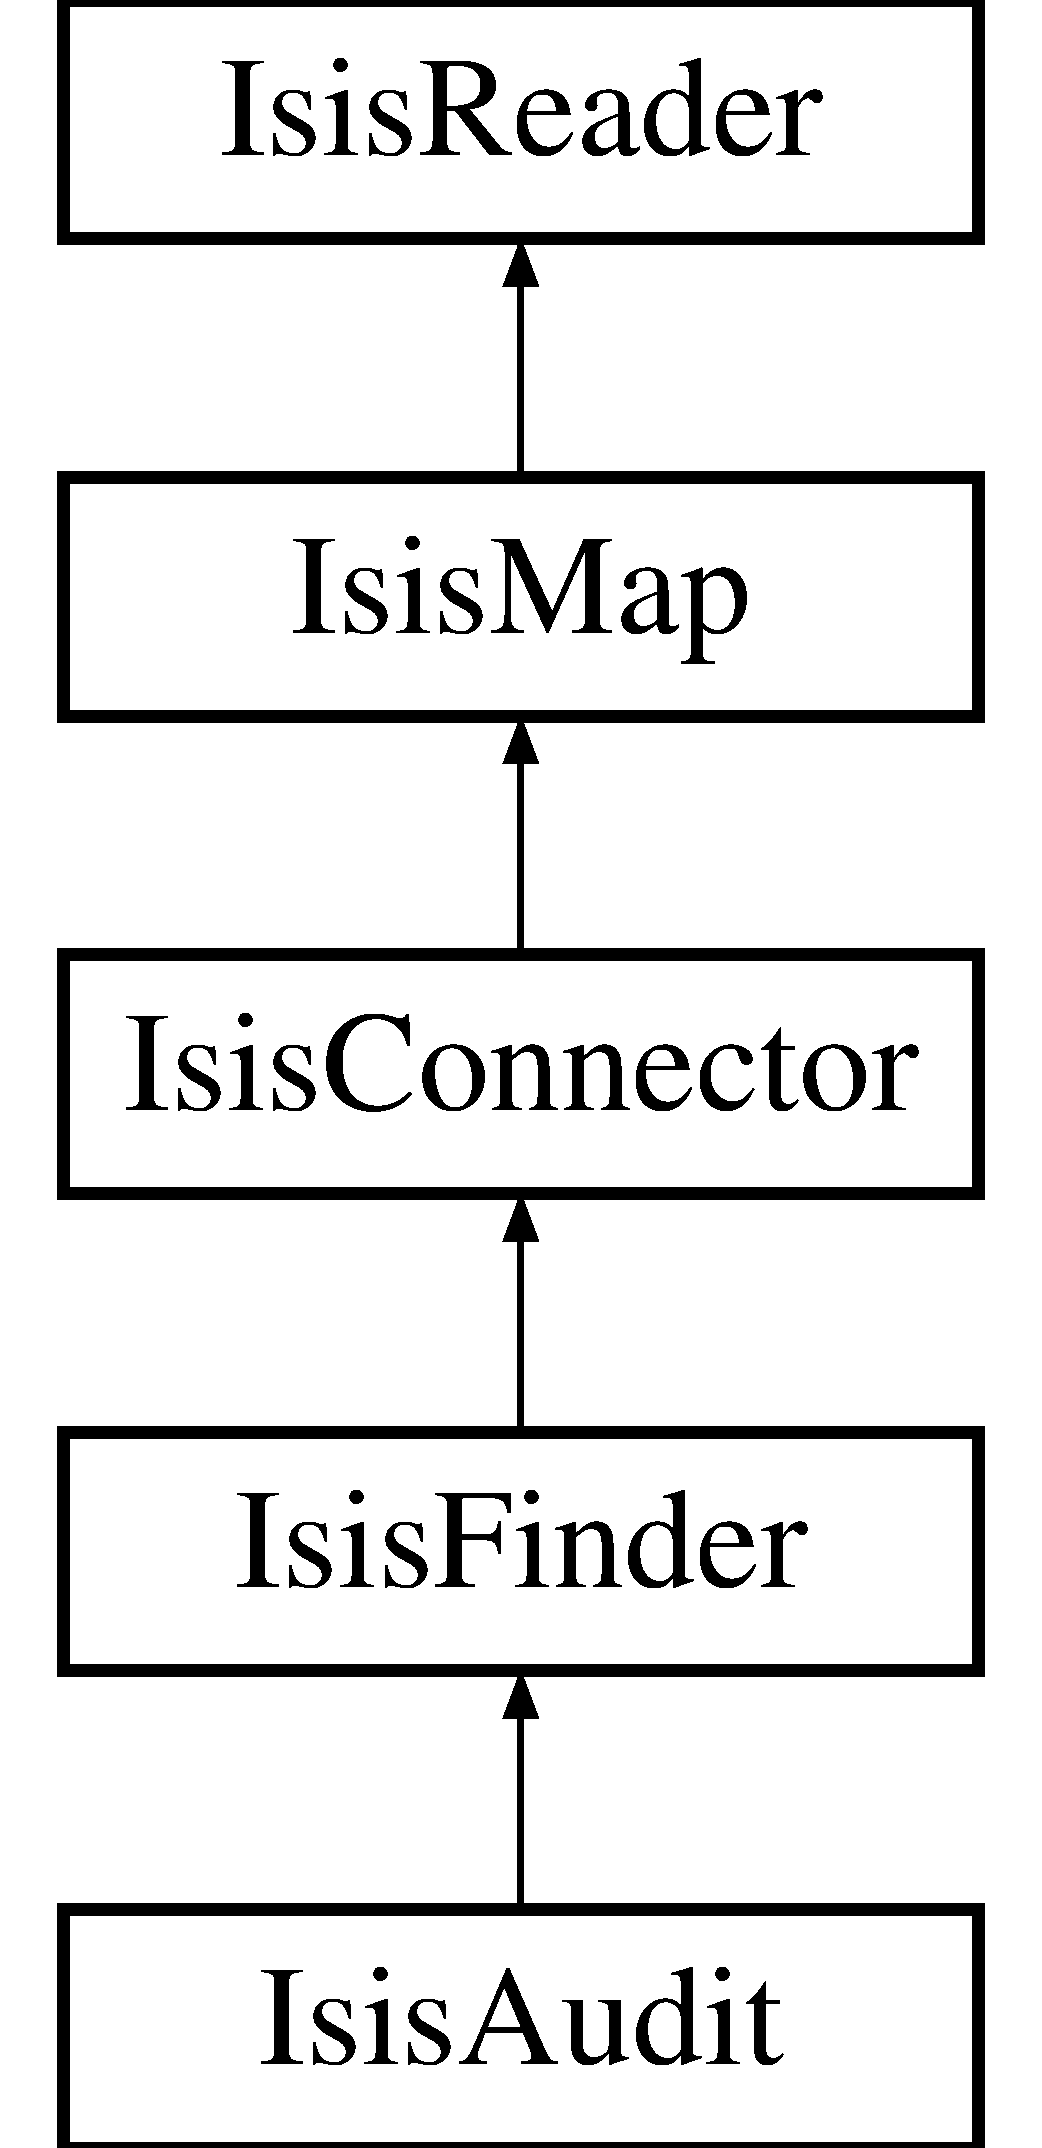
\includegraphics[height=5cm]{classIsisMap}
\end{center}
\end{figure}
\subsection*{Public Member Functions}
\begin{DoxyCompactItemize}
\item 
\hyperlink{classIsisMap_af689f27e67b0b38a3e880ead17a487f5}{getMainItemName} (\$field)
\item 
\hyperlink{classIsisMap_ad0b61ec2fbfb011db4bf89c5f54efab4}{getSubfieldList} (\$field)
\item 
\hyperlink{classIsisMap_a29eb2c45b51f95fdfb9ff7af770ca6ce}{getMap} (\$field, \$subfield=NULL)
\item 
\hyperlink{classIsisMap_a62b933be483fb6704e12e41f10286cd5}{getMapType} (\$field)
\item 
\hyperlink{classIsisMap_af94e1fc5d73a6272f04a60c0acaeb409}{fieldHasMap} (\$field)
\item 
\hyperlink{classIsisMap_ab5493af644e529c11a3c3e6edc37c3b9}{subfieldHasMap} (\$field, \$subfield)
\item 
\hyperlink{classIsisMap_ae5d904b8407b38751656715fb9efd7cf}{getSubfieldKey} (\$field, \$subfield)
\item 
\hyperlink{classIsisMap_a994934784caa4149737bda55160a459f}{getItemKey} (\$field, \$item)
\item 
\hyperlink{classIsisMap_ac6a4eed048ddfa62c76e6d813754af81}{getFieldKey} (\$field)
\item 
\hyperlink{classIsisMap_aee1953b6e46b1612c725b2da82414d14}{getFieldArray} (\$field\_\-key)
\item 
\hyperlink{classIsisMap_a83ffdd84c385513a09e5ab523a44d6f2}{getSubfieldName} (\$field\_\-key, \$subfield\_\-key)
\item 
\hyperlink{classIsisMap_ae41313537e399f15ff16a4db887cf5b9}{getFieldName} (\$field\_\-key)
\end{DoxyCompactItemize}
\subsection*{Static Public Member Functions}
\begin{DoxyCompactItemize}
\item 
static \hyperlink{classIsisMap_af80aedabfeca623a9022dfcbc95d591c}{methodName} (\$type)
\item 
static \hyperlink{classIsisMap_ae2abf0591a4862f537fa23537ffca705}{normalizeFieldName} (\$name)
\item 
static \hyperlink{classIsisMap_a7f1b9b1cce7a02dea704a40ca85e2117}{mapName} (\$name)
\end{DoxyCompactItemize}


\subsection{Detailed Description}
Provides mappings and schema functionalities around \hyperlink{classCinisis}{Cinisis}. 

\subsection{Member Function Documentation}
\hypertarget{classIsisMap_af94e1fc5d73a6272f04a60c0acaeb409}{
\index{IsisMap@{IsisMap}!fieldHasMap@{fieldHasMap}}
\index{fieldHasMap@{fieldHasMap}!IsisMap@{IsisMap}}
\subsubsection[{fieldHasMap}]{\setlength{\rightskip}{0pt plus 5cm}IsisMap::fieldHasMap (\$ {\em field})}}
\label{classIsisMap_af94e1fc5d73a6272f04a60c0acaeb409}
Check on an ISIS schema whether a field has a map.


\begin{DoxyParams}{Parameters}
\item[{\em \$field}]Field array.\end{DoxyParams}
\begin{DoxyReturn}{Returns}
TRUE if field has a map, FALSE otherwise. 
\end{DoxyReturn}
\hypertarget{classIsisMap_aee1953b6e46b1612c725b2da82414d14}{
\index{IsisMap@{IsisMap}!getFieldArray@{getFieldArray}}
\index{getFieldArray@{getFieldArray}!IsisMap@{IsisMap}}
\subsubsection[{getFieldArray}]{\setlength{\rightskip}{0pt plus 5cm}IsisMap::getFieldArray (\$ {\em field\_\-key})}}
\label{classIsisMap_aee1953b6e46b1612c725b2da82414d14}
Get the array which defines a field.


\begin{DoxyParams}{Parameters}
\item[{\em \$field\_\-key}]Field key.\end{DoxyParams}
\begin{DoxyReturn}{Returns}
Field array. 
\end{DoxyReturn}
\hypertarget{classIsisMap_ac6a4eed048ddfa62c76e6d813754af81}{
\index{IsisMap@{IsisMap}!getFieldKey@{getFieldKey}}
\index{getFieldKey@{getFieldKey}!IsisMap@{IsisMap}}
\subsubsection[{getFieldKey}]{\setlength{\rightskip}{0pt plus 5cm}IsisMap::getFieldKey (\$ {\em field})}}
\label{classIsisMap_ac6a4eed048ddfa62c76e6d813754af81}
Get the key of a field entry.


\begin{DoxyParams}{Parameters}
\item[{\em \$field}]Field array.\end{DoxyParams}
\begin{DoxyReturn}{Returns}
Field key. 
\end{DoxyReturn}
\hypertarget{classIsisMap_ae41313537e399f15ff16a4db887cf5b9}{
\index{IsisMap@{IsisMap}!getFieldName@{getFieldName}}
\index{getFieldName@{getFieldName}!IsisMap@{IsisMap}}
\subsubsection[{getFieldName}]{\setlength{\rightskip}{0pt plus 5cm}IsisMap::getFieldName (\$ {\em field\_\-key})}}
\label{classIsisMap_ae41313537e399f15ff16a4db887cf5b9}
Get a field name.


\begin{DoxyParams}{Parameters}
\item[{\em \$field\_\-key}]Field key.\end{DoxyParams}
\begin{DoxyReturn}{Returns}
Field name. 
\end{DoxyReturn}
\hypertarget{classIsisMap_a994934784caa4149737bda55160a459f}{
\index{IsisMap@{IsisMap}!getItemKey@{getItemKey}}
\index{getItemKey@{getItemKey}!IsisMap@{IsisMap}}
\subsubsection[{getItemKey}]{\setlength{\rightskip}{0pt plus 5cm}IsisMap::getItemKey (\$ {\em field}, \/  \$ {\em item})}}
\label{classIsisMap_a994934784caa4149737bda55160a459f}
Get the item key.


\begin{DoxyParams}{Parameters}
\item[{\em \$field}]Field array.\item[{\em \$item}]Item name.\end{DoxyParams}
\begin{DoxyReturn}{Returns}
Item key. 
\end{DoxyReturn}
\hypertarget{classIsisMap_af689f27e67b0b38a3e880ead17a487f5}{
\index{IsisMap@{IsisMap}!getMainItemName@{getMainItemName}}
\index{getMainItemName@{getMainItemName}!IsisMap@{IsisMap}}
\subsubsection[{getMainItemName}]{\setlength{\rightskip}{0pt plus 5cm}IsisMap::getMainItemName (\$ {\em field})}}
\label{classIsisMap_af689f27e67b0b38a3e880ead17a487f5}
Get the main field name.


\begin{DoxyParams}{Parameters}
\item[{\em \$field}]Field data from ISIS database schema.\end{DoxyParams}
\begin{DoxyReturn}{Returns}
Main field name. 
\end{DoxyReturn}
\hypertarget{classIsisMap_a29eb2c45b51f95fdfb9ff7af770ca6ce}{
\index{IsisMap@{IsisMap}!getMap@{getMap}}
\index{getMap@{getMap}!IsisMap@{IsisMap}}
\subsubsection[{getMap}]{\setlength{\rightskip}{0pt plus 5cm}IsisMap::getMap (\$ {\em field}, \/  \$ {\em subfield} = {\ttfamily NULL})}}
\label{classIsisMap_a29eb2c45b51f95fdfb9ff7af770ca6ce}
Determine which model field an ISIS db field should be mapped to. When importing an ISIS database to another system, a mapping provided in the database schema can be used to put the originating entries (fields and subfields) in the right place at the destination database.

Map format:

map: type: relation

map: type: value field: dest subfields: a: dest b: dest

Examples:

map: type: Performer

map: type: value field: title subfields: a: subtitle


\begin{DoxyParams}{Parameters}
\item[{\em \$field}]Field array.\item[{\em \$subfield}]Subfield name.\end{DoxyParams}
\begin{DoxyReturn}{Returns}
A map destination to the field or subfield. 
\end{DoxyReturn}
\hypertarget{classIsisMap_a62b933be483fb6704e12e41f10286cd5}{
\index{IsisMap@{IsisMap}!getMapType@{getMapType}}
\index{getMapType@{getMapType}!IsisMap@{IsisMap}}
\subsubsection[{getMapType}]{\setlength{\rightskip}{0pt plus 5cm}IsisMap::getMapType (\$ {\em field})}}
\label{classIsisMap_a62b933be483fb6704e12e41f10286cd5}
Get the mapping type of a given field.


\begin{DoxyParams}{Parameters}
\item[{\em \$field}]Field array.\end{DoxyParams}
\begin{DoxyReturn}{Returns}
The mapping type. 
\end{DoxyReturn}
\hypertarget{classIsisMap_ae5d904b8407b38751656715fb9efd7cf}{
\index{IsisMap@{IsisMap}!getSubfieldKey@{getSubfieldKey}}
\index{getSubfieldKey@{getSubfieldKey}!IsisMap@{IsisMap}}
\subsubsection[{getSubfieldKey}]{\setlength{\rightskip}{0pt plus 5cm}IsisMap::getSubfieldKey (\$ {\em field}, \/  \$ {\em subfield})}}
\label{classIsisMap_ae5d904b8407b38751656715fb9efd7cf}
Get the key of a subfield entry.


\begin{DoxyParams}{Parameters}
\item[{\em \$field}]Field array.\item[{\em \$subfield}]Subfield name.\end{DoxyParams}
\begin{DoxyReturn}{Returns}
Subfield key. 
\end{DoxyReturn}
\hypertarget{classIsisMap_ad0b61ec2fbfb011db4bf89c5f54efab4}{
\index{IsisMap@{IsisMap}!getSubfieldList@{getSubfieldList}}
\index{getSubfieldList@{getSubfieldList}!IsisMap@{IsisMap}}
\subsubsection[{getSubfieldList}]{\setlength{\rightskip}{0pt plus 5cm}IsisMap::getSubfieldList (\$ {\em field})}}
\label{classIsisMap_ad0b61ec2fbfb011db4bf89c5f54efab4}
Get the list of subfields from a given field.


\begin{DoxyParams}{Parameters}
\item[{\em \$field}]Field array. \end{DoxyParams}
\hypertarget{classIsisMap_a83ffdd84c385513a09e5ab523a44d6f2}{
\index{IsisMap@{IsisMap}!getSubfieldName@{getSubfieldName}}
\index{getSubfieldName@{getSubfieldName}!IsisMap@{IsisMap}}
\subsubsection[{getSubfieldName}]{\setlength{\rightskip}{0pt plus 5cm}IsisMap::getSubfieldName (\$ {\em field\_\-key}, \/  \$ {\em subfield\_\-key})}}
\label{classIsisMap_a83ffdd84c385513a09e5ab523a44d6f2}
Get a subfield name.


\begin{DoxyParams}{Parameters}
\item[{\em \$field\_\-key}]Field key.\item[{\em \$subfield\_\-key}]Subfield key.\end{DoxyParams}
\begin{DoxyReturn}{Returns}
Subfield name. 
\end{DoxyReturn}
\hypertarget{classIsisMap_a7f1b9b1cce7a02dea704a40ca85e2117}{
\index{IsisMap@{IsisMap}!mapName@{mapName}}
\index{mapName@{mapName}!IsisMap@{IsisMap}}
\subsubsection[{mapName}]{\setlength{\rightskip}{0pt plus 5cm}static IsisMap::mapName (\$ {\em name})\hspace{0.3cm}{\ttfamily  \mbox{[}static\mbox{]}}}}
\label{classIsisMap_a7f1b9b1cce7a02dea704a40ca85e2117}
Build a map name.


\begin{DoxyParams}{Parameters}
\item[{\em \$name}]Field name\end{DoxyParams}
\begin{DoxyReturn}{Returns}
Map name 
\end{DoxyReturn}
\hypertarget{classIsisMap_af80aedabfeca623a9022dfcbc95d591c}{
\index{IsisMap@{IsisMap}!methodName@{methodName}}
\index{methodName@{methodName}!IsisMap@{IsisMap}}
\subsubsection[{methodName}]{\setlength{\rightskip}{0pt plus 5cm}static IsisMap::methodName (\$ {\em type})\hspace{0.3cm}{\ttfamily  \mbox{[}static\mbox{]}}}}
\label{classIsisMap_af80aedabfeca623a9022dfcbc95d591c}
Guess a method name from a type.


\begin{DoxyParams}{Parameters}
\item[{\em \$type}]Mapping type.\end{DoxyParams}
\begin{DoxyReturn}{Returns}
Method name. 
\end{DoxyReturn}
\hypertarget{classIsisMap_ae2abf0591a4862f537fa23537ffca705}{
\index{IsisMap@{IsisMap}!normalizeFieldName@{normalizeFieldName}}
\index{normalizeFieldName@{normalizeFieldName}!IsisMap@{IsisMap}}
\subsubsection[{normalizeFieldName}]{\setlength{\rightskip}{0pt plus 5cm}static IsisMap::normalizeFieldName (\$ {\em name})\hspace{0.3cm}{\ttfamily  \mbox{[}static\mbox{]}}}}
\label{classIsisMap_ae2abf0591a4862f537fa23537ffca705}
Normalize field names.


\begin{DoxyParams}{Parameters}
\item[{\em \$name}]Field name\end{DoxyParams}
\begin{DoxyReturn}{Returns}
Normalized field name 
\end{DoxyReturn}
\hypertarget{classIsisMap_ab5493af644e529c11a3c3e6edc37c3b9}{
\index{IsisMap@{IsisMap}!subfieldHasMap@{subfieldHasMap}}
\index{subfieldHasMap@{subfieldHasMap}!IsisMap@{IsisMap}}
\subsubsection[{subfieldHasMap}]{\setlength{\rightskip}{0pt plus 5cm}IsisMap::subfieldHasMap (\$ {\em field}, \/  \$ {\em subfield})}}
\label{classIsisMap_ab5493af644e529c11a3c3e6edc37c3b9}
Check on an ISIS schema whether a subfield has a map.


\begin{DoxyParams}{Parameters}
\item[{\em \$field}]Field array.\item[{\em \$subfield}]Subfield name.\end{DoxyParams}
\begin{DoxyReturn}{Returns}
TRUE if subfield has a map, FALSE otherwise. 
\end{DoxyReturn}


The documentation for this class was generated from the following file:\begin{DoxyCompactItemize}
\item 
classes/IsisMap.php\end{DoxyCompactItemize}

\hypertarget{classIsisMethodIterator}{
\section{IsisMethodIterator Class Reference}
\label{classIsisMethodIterator}\index{IsisMethodIterator@{IsisMethodIterator}}
}
\subsection*{Public Member Functions}
\begin{DoxyCompactItemize}
\item 
\hyperlink{classIsisMethodIterator_a1cf2e69c03a092839a2494264ca2ed07}{\_\-\_\-construct} (\$class)
\item 
\hyperlink{classIsisMethodIterator_a1a0ee1617a50e6aa57fe80cd0c2023df}{rewind} ()
\item 
\hyperlink{classIsisMethodIterator_ad750f5dd57dcb6480f64f9ac703492fc}{key} ()
\item 
\hyperlink{classIsisMethodIterator_a1d7236d349cd282c4c0ff6ec8f186e93}{current} ()
\item 
\hyperlink{classIsisMethodIterator_a8a02e17d6597ba1f199bd82ab9fc1b32}{next} ()
\item 
\hyperlink{classIsisMethodIterator_acb2ac4c3a336d9c6c25d97bd47f60759}{valid} ()
\end{DoxyCompactItemize}


\subsection{Detailed Description}
Iterates over all callable methods for database mapping. 

\subsection{Constructor \& Destructor Documentation}
\hypertarget{classIsisMethodIterator_a1cf2e69c03a092839a2494264ca2ed07}{
\index{IsisMethodIterator@{IsisMethodIterator}!\_\-\_\-construct@{\_\-\_\-construct}}
\index{\_\-\_\-construct@{\_\-\_\-construct}!IsisMethodIterator@{IsisMethodIterator}}
\subsubsection[{\_\-\_\-construct}]{\setlength{\rightskip}{0pt plus 5cm}IsisMethodIterator::\_\-\_\-construct (\$ {\em class})}}
\label{classIsisMethodIterator_a1cf2e69c03a092839a2494264ca2ed07}
Constructor.


\begin{DoxyParams}{Parameters}
\item[{\em \$class}]Instance of \hyperlink{classIsisConnector}{IsisConnector} or child class. \end{DoxyParams}


\subsection{Member Function Documentation}
\hypertarget{classIsisMethodIterator_a1d7236d349cd282c4c0ff6ec8f186e93}{
\index{IsisMethodIterator@{IsisMethodIterator}!current@{current}}
\index{current@{current}!IsisMethodIterator@{IsisMethodIterator}}
\subsubsection[{current}]{\setlength{\rightskip}{0pt plus 5cm}IsisMethodIterator::current ()}}
\label{classIsisMethodIterator_a1d7236d349cd282c4c0ff6ec8f186e93}
Return the current element. \hypertarget{classIsisMethodIterator_ad750f5dd57dcb6480f64f9ac703492fc}{
\index{IsisMethodIterator@{IsisMethodIterator}!key@{key}}
\index{key@{key}!IsisMethodIterator@{IsisMethodIterator}}
\subsubsection[{key}]{\setlength{\rightskip}{0pt plus 5cm}IsisMethodIterator::key ()}}
\label{classIsisMethodIterator_ad750f5dd57dcb6480f64f9ac703492fc}
Return the key of the current element. \hypertarget{classIsisMethodIterator_a8a02e17d6597ba1f199bd82ab9fc1b32}{
\index{IsisMethodIterator@{IsisMethodIterator}!next@{next}}
\index{next@{next}!IsisMethodIterator@{IsisMethodIterator}}
\subsubsection[{next}]{\setlength{\rightskip}{0pt plus 5cm}IsisMethodIterator::next ()}}
\label{classIsisMethodIterator_a8a02e17d6597ba1f199bd82ab9fc1b32}
Move forward to next element. The method should be callable, otherwise we move to the next position. \hypertarget{classIsisMethodIterator_a1a0ee1617a50e6aa57fe80cd0c2023df}{
\index{IsisMethodIterator@{IsisMethodIterator}!rewind@{rewind}}
\index{rewind@{rewind}!IsisMethodIterator@{IsisMethodIterator}}
\subsubsection[{rewind}]{\setlength{\rightskip}{0pt plus 5cm}IsisMethodIterator::rewind ()}}
\label{classIsisMethodIterator_a1a0ee1617a50e6aa57fe80cd0c2023df}
Rewind the Iterator to the first valid element. \hypertarget{classIsisMethodIterator_acb2ac4c3a336d9c6c25d97bd47f60759}{
\index{IsisMethodIterator@{IsisMethodIterator}!valid@{valid}}
\index{valid@{valid}!IsisMethodIterator@{IsisMethodIterator}}
\subsubsection[{valid}]{\setlength{\rightskip}{0pt plus 5cm}IsisMethodIterator::valid ()}}
\label{classIsisMethodIterator_acb2ac4c3a336d9c6c25d97bd47f60759}
Check if there is a current element after calls to \hyperlink{classIsisMethodIterator_a1a0ee1617a50e6aa57fe80cd0c2023df}{rewind()} or \hyperlink{classIsisMethodIterator_a8a02e17d6597ba1f199bd82ab9fc1b32}{next()}. 

The documentation for this class was generated from the following file:\begin{DoxyCompactItemize}
\item 
classes/iterators/IsisMethodIterator.php\end{DoxyCompactItemize}

\hypertarget{classIsisNormalItemFilterIterator}{
\section{IsisNormalItemFilterIterator Class Reference}
\label{classIsisNormalItemFilterIterator}\index{IsisNormalItemFilterIterator@{IsisNormalItemFilterIterator}}
}
\subsection*{Public Member Functions}
\begin{DoxyCompactItemize}
\item 
\hyperlink{classIsisNormalItemFilterIterator_ad3ef2ecdafb6a163a01b199a7e98cd6f}{accept} ()
\end{DoxyCompactItemize}


\subsection{Detailed Description}
Isis normal subfield iterator. Filter out special subfields. 

\subsection{Member Function Documentation}
\hypertarget{classIsisNormalItemFilterIterator_ad3ef2ecdafb6a163a01b199a7e98cd6f}{
\index{IsisNormalItemFilterIterator@{IsisNormalItemFilterIterator}!accept@{accept}}
\index{accept@{accept}!IsisNormalItemFilterIterator@{IsisNormalItemFilterIterator}}
\subsubsection[{accept}]{\setlength{\rightskip}{0pt plus 5cm}IsisNormalItemFilterIterator::accept (
\begin{DoxyParamCaption}
{}
\end{DoxyParamCaption}
)}}
\label{classIsisNormalItemFilterIterator_ad3ef2ecdafb6a163a01b199a7e98cd6f}
Filter out special subfields. 

The documentation for this class was generated from the following file:\begin{DoxyCompactItemize}
\item 
classes/iterators/IsisNormalItemFilterIterator.php\end{DoxyCompactItemize}

\hypertarget{classIsisReader}{
\section{IsisReader Class Reference}
\label{classIsisReader}\index{IsisReader@{IsisReader}}
}
Inheritance diagram for IsisReader:\begin{figure}[H]
\begin{center}
\leavevmode
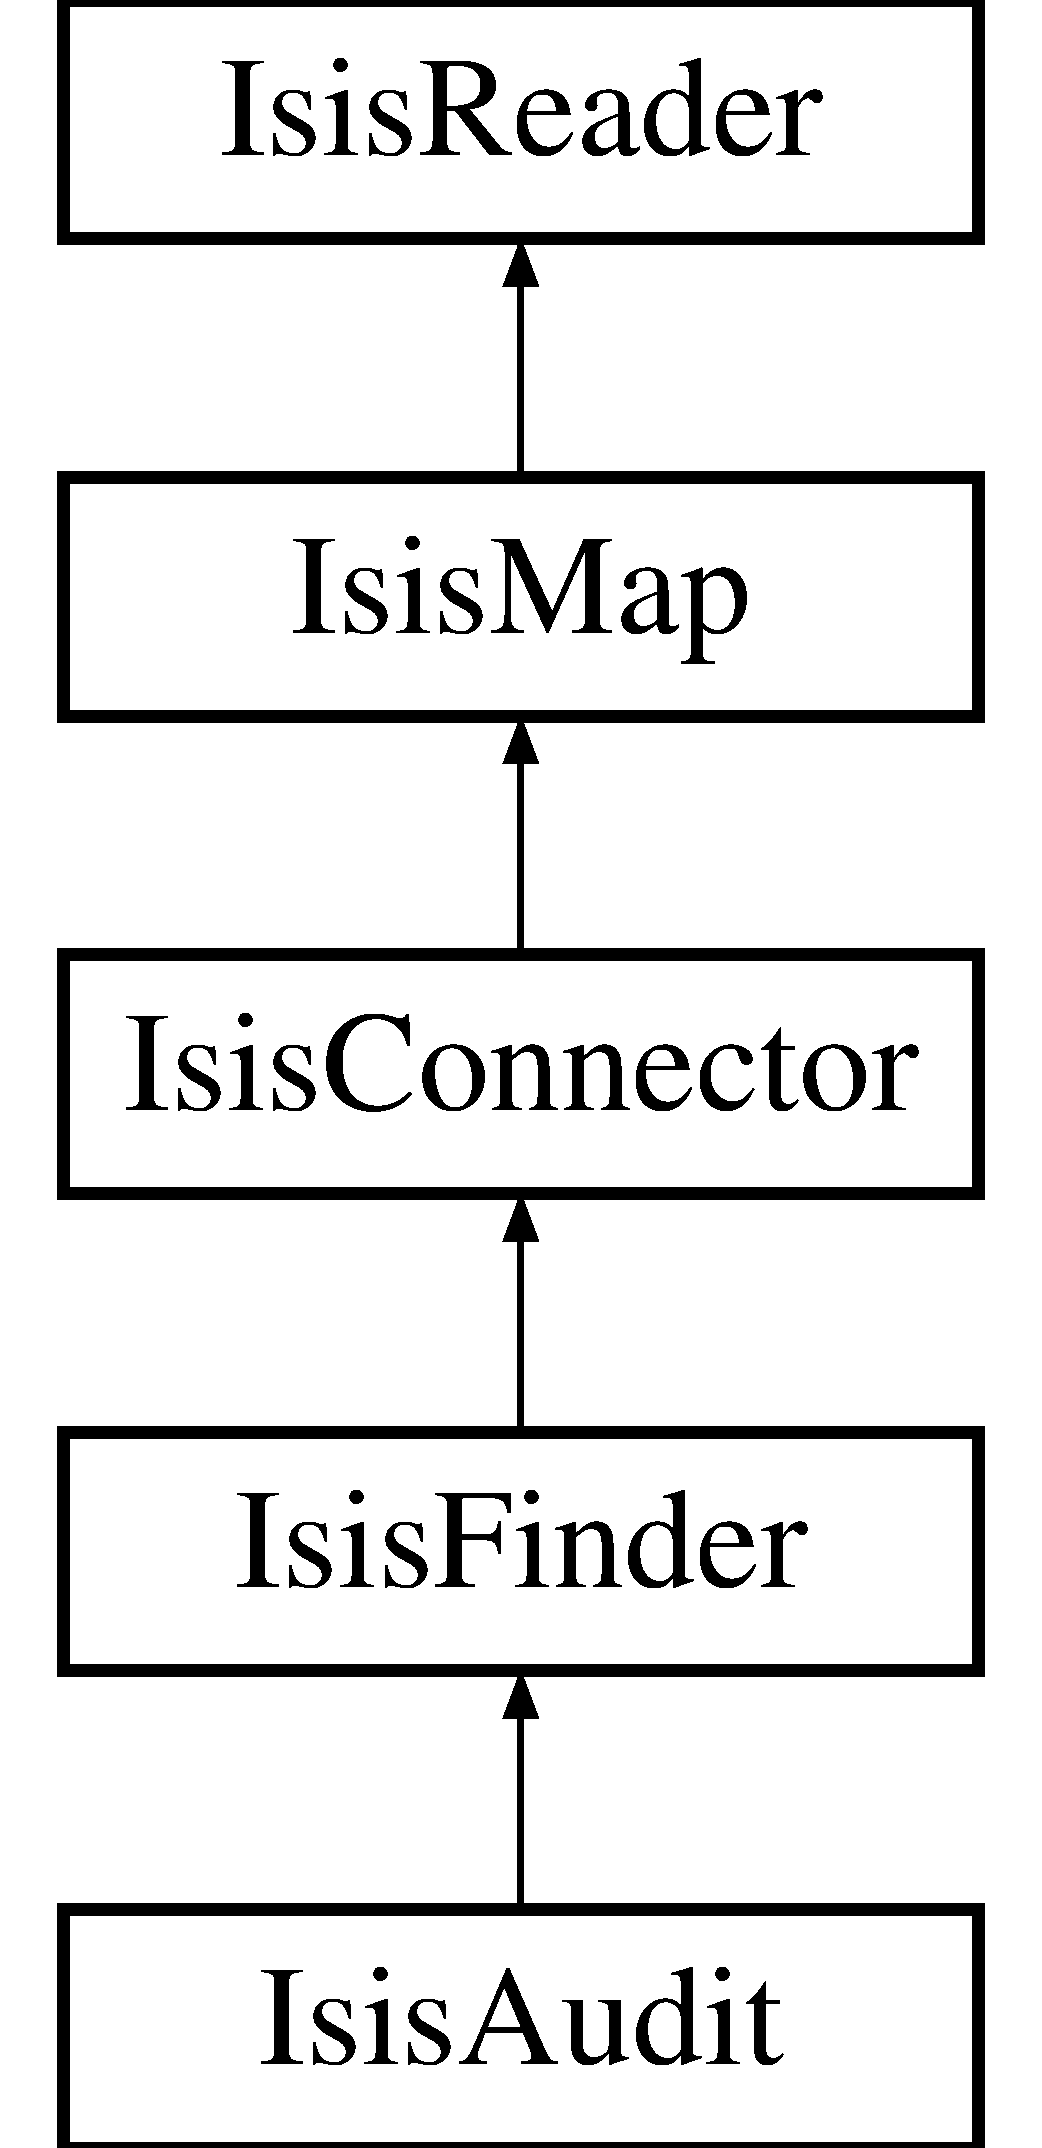
\includegraphics[height=5.000000cm]{classIsisReader}
\end{center}
\end{figure}
\subsection*{Public Member Functions}
\begin{DoxyCompactItemize}
\item 
\hyperlink{classIsisReader_a70d1444cf56269795b4947dd82b2a4ac}{\_\-\_\-construct} (\$config=null)
\item 
\hyperlink{classIsisReader_afa6e3d3d94854913e5ed2604919d2316}{open} (\$config)
\item 
\hyperlink{classIsisReader_a630791a319bec2bc55d0102cbb7f93df}{read} (\$entry)
\item 
\hyperlink{classIsisReader_a99ce7b10b2997dad6a64558ac1f9f10e}{removeBrackets} (\$value)
\item 
\hyperlink{classIsisReader_acba8842f0033356fff66c0f88391921e}{removeBracketsCallback} (\&\$value=NULL)
\item 
\hyperlink{classIsisReader_a60ece3bbe11a2b4ac6afa6e65f282724}{removeBracketsFromArray} (\&\$values)
\item 
\hyperlink{classIsisReader_a4610ebcf69c197e2c596965e2dc0358e}{explodeBrackets} (\$subject)
\item 
\hyperlink{classIsisReader_aa6099ed6bd276b32bd7bba184f144529}{filterBrackets} (\$values)
\item 
\hyperlink{classIsisReader_a109a6ef49b2190bfbcee796dae954baf}{hasBrackets} (\$value)
\item 
\hyperlink{classIsisReader_a3cc08df25da082046d496db93778709b}{explodeValue} (\$value)
\item 
\hyperlink{classIsisReader_ae65e172e3b5c9ac3c8a5e1352ba80904}{joinSubfields} ()
\end{DoxyCompactItemize}


\subsection{Detailed Description}
Provides basic Isis read capabilities around \hyperlink{classCinisis}{Cinisis}. 

\subsection{Constructor \& Destructor Documentation}
\hypertarget{classIsisReader_a70d1444cf56269795b4947dd82b2a4ac}{
\index{IsisReader@{IsisReader}!\_\-\_\-construct@{\_\-\_\-construct}}
\index{\_\-\_\-construct@{\_\-\_\-construct}!IsisReader@{IsisReader}}
\subsubsection[{\_\-\_\-construct}]{\setlength{\rightskip}{0pt plus 5cm}IsisReader::\_\-\_\-construct (
\begin{DoxyParamCaption}
\item[{\$}]{ config = {\ttfamily null}}
\end{DoxyParamCaption}
)}}
\label{classIsisReader_a70d1444cf56269795b4947dd82b2a4ac}
Constructor. 

\subsection{Member Function Documentation}
\hypertarget{classIsisReader_a4610ebcf69c197e2c596965e2dc0358e}{
\index{IsisReader@{IsisReader}!explodeBrackets@{explodeBrackets}}
\index{explodeBrackets@{explodeBrackets}!IsisReader@{IsisReader}}
\subsubsection[{explodeBrackets}]{\setlength{\rightskip}{0pt plus 5cm}IsisReader::explodeBrackets (
\begin{DoxyParamCaption}
\item[{\$}]{ subject}
\end{DoxyParamCaption}
)}}
\label{classIsisReader_a4610ebcf69c197e2c596965e2dc0358e}
Explode a bracketed string into values. Just strings inside brackets are returned.


\begin{DoxyParams}{Parameters}
\item[{\em \$subject}]Strings containing brackets.\end{DoxyParams}
\begin{DoxyReturn}{Returns}
Array of matched strings. 
\end{DoxyReturn}
\hypertarget{classIsisReader_a3cc08df25da082046d496db93778709b}{
\index{IsisReader@{IsisReader}!explodeValue@{explodeValue}}
\index{explodeValue@{explodeValue}!IsisReader@{IsisReader}}
\subsubsection[{explodeValue}]{\setlength{\rightskip}{0pt plus 5cm}IsisReader::explodeValue (
\begin{DoxyParamCaption}
\item[{\$}]{ value}
\end{DoxyParamCaption}
)}}
\label{classIsisReader_a3cc08df25da082046d496db93778709b}
Explode values from fields or subfields. Split values inside brackets if needed, but then doesn't return any value outside brackets.


\begin{DoxyParams}{Parameters}
\item[{\em \$value}]String with values.\end{DoxyParams}
\begin{DoxyReturn}{Returns}
Array with values. 
\end{DoxyReturn}
\hypertarget{classIsisReader_aa6099ed6bd276b32bd7bba184f144529}{
\index{IsisReader@{IsisReader}!filterBrackets@{filterBrackets}}
\index{filterBrackets@{filterBrackets}!IsisReader@{IsisReader}}
\subsubsection[{filterBrackets}]{\setlength{\rightskip}{0pt plus 5cm}IsisReader::filterBrackets (
\begin{DoxyParamCaption}
\item[{\$}]{ values}
\end{DoxyParamCaption}
)}}
\label{classIsisReader_aa6099ed6bd276b32bd7bba184f144529}
Filter out brackets from strings.


\begin{DoxyParams}{Parameters}
\item[{\em \$values}]String (or array filled with strings) to be filtered.\end{DoxyParams}
\begin{DoxyReturn}{Returns}
Filtered string or array. 
\end{DoxyReturn}
\hypertarget{classIsisReader_a109a6ef49b2190bfbcee796dae954baf}{
\index{IsisReader@{IsisReader}!hasBrackets@{hasBrackets}}
\index{hasBrackets@{hasBrackets}!IsisReader@{IsisReader}}
\subsubsection[{hasBrackets}]{\setlength{\rightskip}{0pt plus 5cm}IsisReader::hasBrackets (
\begin{DoxyParamCaption}
\item[{\$}]{ value}
\end{DoxyParamCaption}
)}}
\label{classIsisReader_a109a6ef49b2190bfbcee796dae954baf}
Check if a string has brackets.


\begin{DoxyParams}{Parameters}
\item[{\em \$value}]String to be compared.\end{DoxyParams}
\begin{DoxyReturn}{Returns}
True if string has brackets, false otherwise. 
\end{DoxyReturn}
\hypertarget{classIsisReader_ae65e172e3b5c9ac3c8a5e1352ba80904}{
\index{IsisReader@{IsisReader}!joinSubfields@{joinSubfields}}
\index{joinSubfields@{joinSubfields}!IsisReader@{IsisReader}}
\subsubsection[{joinSubfields}]{\setlength{\rightskip}{0pt plus 5cm}IsisReader::joinSubfields (
\begin{DoxyParamCaption}
{}
\end{DoxyParamCaption}
)}}
\label{classIsisReader_ae65e172e3b5c9ac3c8a5e1352ba80904}
Whether to join field and subfields in a single array.

\begin{DoxyReturn}{Returns}
Boolean. 
\end{DoxyReturn}
\hypertarget{classIsisReader_afa6e3d3d94854913e5ed2604919d2316}{
\index{IsisReader@{IsisReader}!open@{open}}
\index{open@{open}!IsisReader@{IsisReader}}
\subsubsection[{open}]{\setlength{\rightskip}{0pt plus 5cm}IsisReader::open (
\begin{DoxyParamCaption}
\item[{\$}]{ config}
\end{DoxyParamCaption}
)}}
\label{classIsisReader_afa6e3d3d94854913e5ed2604919d2316}
Open a database.


\begin{DoxyParams}{Parameters}
\item[{\em \$config}]Config file or array. \end{DoxyParams}
\hypertarget{classIsisReader_a630791a319bec2bc55d0102cbb7f93df}{
\index{IsisReader@{IsisReader}!read@{read}}
\index{read@{read}!IsisReader@{IsisReader}}
\subsubsection[{read}]{\setlength{\rightskip}{0pt plus 5cm}IsisReader::read (
\begin{DoxyParamCaption}
\item[{\$}]{ entry}
\end{DoxyParamCaption}
)}}
\label{classIsisReader_a630791a319bec2bc55d0102cbb7f93df}
Alias to \$isis-\/$>$db-\/$>$\hyperlink{classIsisReader_a630791a319bec2bc55d0102cbb7f93df}{read()}.


\begin{DoxyParams}{Parameters}
\item[{\em \$entry}]Row number.\end{DoxyParams}
\begin{DoxyReturn}{Returns}
Resulting data. 
\end{DoxyReturn}
\hypertarget{classIsisReader_a99ce7b10b2997dad6a64558ac1f9f10e}{
\index{IsisReader@{IsisReader}!removeBrackets@{removeBrackets}}
\index{removeBrackets@{removeBrackets}!IsisReader@{IsisReader}}
\subsubsection[{removeBrackets}]{\setlength{\rightskip}{0pt plus 5cm}IsisReader::removeBrackets (
\begin{DoxyParamCaption}
\item[{\$}]{ value}
\end{DoxyParamCaption}
)}}
\label{classIsisReader_a99ce7b10b2997dad6a64558ac1f9f10e}
Remove brackets from strings whithin an array.


\begin{DoxyParams}{Parameters}
\item[{\em \$value}]Array with bracketed strings.\end{DoxyParams}
\begin{DoxyReturn}{Returns}
Array with strings without brackets. 
\end{DoxyReturn}
\hypertarget{classIsisReader_acba8842f0033356fff66c0f88391921e}{
\index{IsisReader@{IsisReader}!removeBracketsCallback@{removeBracketsCallback}}
\index{removeBracketsCallback@{removeBracketsCallback}!IsisReader@{IsisReader}}
\subsubsection[{removeBracketsCallback}]{\setlength{\rightskip}{0pt plus 5cm}IsisReader::removeBracketsCallback (
\begin{DoxyParamCaption}
\item[{\&\$}]{ value = {\ttfamily NULL}}
\end{DoxyParamCaption}
)}}
\label{classIsisReader_acba8842f0033356fff66c0f88391921e}
Remove brackets from strings whithin an array. Callback version


\begin{DoxyParams}{Parameters}
\item[{\em \$value}]Array with bracketed strings. \end{DoxyParams}
\hypertarget{classIsisReader_a60ece3bbe11a2b4ac6afa6e65f282724}{
\index{IsisReader@{IsisReader}!removeBracketsFromArray@{removeBracketsFromArray}}
\index{removeBracketsFromArray@{removeBracketsFromArray}!IsisReader@{IsisReader}}
\subsubsection[{removeBracketsFromArray}]{\setlength{\rightskip}{0pt plus 5cm}IsisReader::removeBracketsFromArray (
\begin{DoxyParamCaption}
\item[{\&\$}]{ values}
\end{DoxyParamCaption}
)}}
\label{classIsisReader_a60ece3bbe11a2b4ac6afa6e65f282724}
Remove brackets from strings whithin an array.


\begin{DoxyParams}{Parameters}
\item[{\em \&\$values}]Array with bracketed strings. \end{DoxyParams}


The documentation for this class was generated from the following file:\begin{DoxyCompactItemize}
\item 
classes/IsisReader.php\end{DoxyCompactItemize}

\hypertarget{classIsisRowIterator}{
\section{IsisRowIterator Class Reference}
\label{classIsisRowIterator}\index{IsisRowIterator@{IsisRowIterator}}
}
\subsection*{Public Member Functions}
\begin{DoxyCompactItemize}
\item 
\hyperlink{classIsisRowIterator_acaab99d2bf18f6f958ddf07db55cb15d}{\_\-\_\-construct} (\$class, \$field)
\item 
\hyperlink{classIsisRowIterator_a5ef72f942cc738bf24cf251018c28edf}{rewind} ()
\item 
\hyperlink{classIsisRowIterator_a96f65bca7f2e048a449e6f316d802e6f}{key} ()
\item 
\hyperlink{classIsisRowIterator_abe18cfd484f70348fb5832444186b10d}{current} ()
\item 
\hyperlink{classIsisRowIterator_ad084ce947a265969f738e7d7dc8a1853}{next} ()
\item 
\hyperlink{classIsisRowIterator_a69cb2b1c6e8feaffcfe65363a9178b72}{valid} ()
\end{DoxyCompactItemize}


\subsection{Detailed Description}
Iterates over all rows from a field result. 

\subsection{Constructor \& Destructor Documentation}
\hypertarget{classIsisRowIterator_acaab99d2bf18f6f958ddf07db55cb15d}{
\index{IsisRowIterator@{IsisRowIterator}!\_\-\_\-construct@{\_\-\_\-construct}}
\index{\_\-\_\-construct@{\_\-\_\-construct}!IsisRowIterator@{IsisRowIterator}}
\subsubsection[{\_\-\_\-construct}]{\setlength{\rightskip}{0pt plus 5cm}IsisRowIterator::\_\-\_\-construct (\$ {\em class}, \/  \$ {\em field})}}
\label{classIsisRowIterator_acaab99d2bf18f6f958ddf07db55cb15d}
Constructor.


\begin{DoxyParams}{Parameters}
\item[{\em \$class}]Instance of \hyperlink{classIsisConnector}{IsisConnector} or child class.\item[{\em \$field}]Field to iterate over. \end{DoxyParams}


\subsection{Member Function Documentation}
\hypertarget{classIsisRowIterator_abe18cfd484f70348fb5832444186b10d}{
\index{IsisRowIterator@{IsisRowIterator}!current@{current}}
\index{current@{current}!IsisRowIterator@{IsisRowIterator}}
\subsubsection[{current}]{\setlength{\rightskip}{0pt plus 5cm}IsisRowIterator::current ()}}
\label{classIsisRowIterator_abe18cfd484f70348fb5832444186b10d}
Return the current element. \hypertarget{classIsisRowIterator_a96f65bca7f2e048a449e6f316d802e6f}{
\index{IsisRowIterator@{IsisRowIterator}!key@{key}}
\index{key@{key}!IsisRowIterator@{IsisRowIterator}}
\subsubsection[{key}]{\setlength{\rightskip}{0pt plus 5cm}IsisRowIterator::key ()}}
\label{classIsisRowIterator_a96f65bca7f2e048a449e6f316d802e6f}
Return the key of the current element. \hypertarget{classIsisRowIterator_ad084ce947a265969f738e7d7dc8a1853}{
\index{IsisRowIterator@{IsisRowIterator}!next@{next}}
\index{next@{next}!IsisRowIterator@{IsisRowIterator}}
\subsubsection[{next}]{\setlength{\rightskip}{0pt plus 5cm}IsisRowIterator::next ()}}
\label{classIsisRowIterator_ad084ce947a265969f738e7d7dc8a1853}
Move forward to next element. \hypertarget{classIsisRowIterator_a5ef72f942cc738bf24cf251018c28edf}{
\index{IsisRowIterator@{IsisRowIterator}!rewind@{rewind}}
\index{rewind@{rewind}!IsisRowIterator@{IsisRowIterator}}
\subsubsection[{rewind}]{\setlength{\rightskip}{0pt plus 5cm}IsisRowIterator::rewind ()}}
\label{classIsisRowIterator_a5ef72f942cc738bf24cf251018c28edf}
Rewind the Iterator to the first element. \hypertarget{classIsisRowIterator_a69cb2b1c6e8feaffcfe65363a9178b72}{
\index{IsisRowIterator@{IsisRowIterator}!valid@{valid}}
\index{valid@{valid}!IsisRowIterator@{IsisRowIterator}}
\subsubsection[{valid}]{\setlength{\rightskip}{0pt plus 5cm}IsisRowIterator::valid ()}}
\label{classIsisRowIterator_a69cb2b1c6e8feaffcfe65363a9178b72}
Check if there is a current element after calls to \hyperlink{classIsisRowIterator_a5ef72f942cc738bf24cf251018c28edf}{rewind()} or \hyperlink{classIsisRowIterator_ad084ce947a265969f738e7d7dc8a1853}{next()}. 

The documentation for this class was generated from the following file:\begin{DoxyCompactItemize}
\item 
classes/iterators/IsisRowIterator.php\end{DoxyCompactItemize}

\hypertarget{classIsisSubfieldIterator}{
\section{IsisSubfieldIterator Class Reference}
\label{classIsisSubfieldIterator}\index{IsisSubfieldIterator@{IsisSubfieldIterator}}
}
\subsection*{Public Member Functions}
\begin{DoxyCompactItemize}
\item 
\hyperlink{classIsisSubfieldIterator_adc5472ca67d20defcab9eba45975dc29}{\_\-\_\-construct} (\$class, \$field, \$main=false)
\item 
\hyperlink{classIsisSubfieldIterator_a971b36317fab4fc07573f215a118fb40}{rewind} ()
\item 
\hyperlink{classIsisSubfieldIterator_a4ee62ad436a7c4ec1dac0c0c5d2a2c85}{key} ()
\item 
\hyperlink{classIsisSubfieldIterator_a7c31b7e8db31e1465d29fb58b2448bd8}{current} ()
\item 
\hyperlink{classIsisSubfieldIterator_a74363e3dbfbde6d409b8ba3b70fc9371}{next} ()
\item 
\hyperlink{classIsisSubfieldIterator_a1934438bfdfa1827e6bcc71d3c90f2db}{valid} ()
\end{DoxyCompactItemize}


\subsection{Detailed Description}
Isis subfield iterator. Iterates over subfields for each result row. 

\subsection{Constructor \& Destructor Documentation}
\hypertarget{classIsisSubfieldIterator_adc5472ca67d20defcab9eba45975dc29}{
\index{IsisSubfieldIterator@{IsisSubfieldIterator}!\_\-\_\-construct@{\_\-\_\-construct}}
\index{\_\-\_\-construct@{\_\-\_\-construct}!IsisSubfieldIterator@{IsisSubfieldIterator}}
\subsubsection[{\_\-\_\-construct}]{\setlength{\rightskip}{0pt plus 5cm}IsisSubfieldIterator::\_\-\_\-construct (
\begin{DoxyParamCaption}
\item[{\$}]{ class, }
\item[{\$}]{ field, }
\item[{\$}]{ main = {\ttfamily false}}
\end{DoxyParamCaption}
)}}
\label{classIsisSubfieldIterator_adc5472ca67d20defcab9eba45975dc29}
Constructor.


\begin{DoxyParams}{Parameters}
\item[{\em \$class}]Instance of \hyperlink{classIsisConnector}{IsisConnector} or child class.\item[{\em \$field}]Field to iterate over.\item[{\em \$main}]Control to which subfield the main field should be mapped to. By default no mapping is made. \end{DoxyParams}


\subsection{Member Function Documentation}
\hypertarget{classIsisSubfieldIterator_a7c31b7e8db31e1465d29fb58b2448bd8}{
\index{IsisSubfieldIterator@{IsisSubfieldIterator}!current@{current}}
\index{current@{current}!IsisSubfieldIterator@{IsisSubfieldIterator}}
\subsubsection[{current}]{\setlength{\rightskip}{0pt plus 5cm}IsisSubfieldIterator::current (
\begin{DoxyParamCaption}
{}
\end{DoxyParamCaption}
)}}
\label{classIsisSubfieldIterator_a7c31b7e8db31e1465d29fb58b2448bd8}
Return the current element. \hypertarget{classIsisSubfieldIterator_a4ee62ad436a7c4ec1dac0c0c5d2a2c85}{
\index{IsisSubfieldIterator@{IsisSubfieldIterator}!key@{key}}
\index{key@{key}!IsisSubfieldIterator@{IsisSubfieldIterator}}
\subsubsection[{key}]{\setlength{\rightskip}{0pt plus 5cm}IsisSubfieldIterator::key (
\begin{DoxyParamCaption}
{}
\end{DoxyParamCaption}
)}}
\label{classIsisSubfieldIterator_a4ee62ad436a7c4ec1dac0c0c5d2a2c85}
Return the key of the current element. \hypertarget{classIsisSubfieldIterator_a74363e3dbfbde6d409b8ba3b70fc9371}{
\index{IsisSubfieldIterator@{IsisSubfieldIterator}!next@{next}}
\index{next@{next}!IsisSubfieldIterator@{IsisSubfieldIterator}}
\subsubsection[{next}]{\setlength{\rightskip}{0pt plus 5cm}IsisSubfieldIterator::next (
\begin{DoxyParamCaption}
{}
\end{DoxyParamCaption}
)}}
\label{classIsisSubfieldIterator_a74363e3dbfbde6d409b8ba3b70fc9371}
Move forward to next element. \hypertarget{classIsisSubfieldIterator_a971b36317fab4fc07573f215a118fb40}{
\index{IsisSubfieldIterator@{IsisSubfieldIterator}!rewind@{rewind}}
\index{rewind@{rewind}!IsisSubfieldIterator@{IsisSubfieldIterator}}
\subsubsection[{rewind}]{\setlength{\rightskip}{0pt plus 5cm}IsisSubfieldIterator::rewind (
\begin{DoxyParamCaption}
{}
\end{DoxyParamCaption}
)}}
\label{classIsisSubfieldIterator_a971b36317fab4fc07573f215a118fb40}
Rewind the Iterator to the first element. \hypertarget{classIsisSubfieldIterator_a1934438bfdfa1827e6bcc71d3c90f2db}{
\index{IsisSubfieldIterator@{IsisSubfieldIterator}!valid@{valid}}
\index{valid@{valid}!IsisSubfieldIterator@{IsisSubfieldIterator}}
\subsubsection[{valid}]{\setlength{\rightskip}{0pt plus 5cm}IsisSubfieldIterator::valid (
\begin{DoxyParamCaption}
{}
\end{DoxyParamCaption}
)}}
\label{classIsisSubfieldIterator_a1934438bfdfa1827e6bcc71d3c90f2db}
Check if there is a current element after calls to \hyperlink{classIsisSubfieldIterator_a971b36317fab4fc07573f215a118fb40}{rewind()} or \hyperlink{classIsisSubfieldIterator_a74363e3dbfbde6d409b8ba3b70fc9371}{next()}. 

The documentation for this class was generated from the following file:\begin{DoxyCompactItemize}
\item 
classes/iterators/IsisSubfieldIterator.php\end{DoxyCompactItemize}

\hypertarget{classIsisValueIterator}{
\section{IsisValueIterator Class Reference}
\label{classIsisValueIterator}\index{IsisValueIterator@{IsisValueIterator}}
}
\subsection*{Public Member Functions}
\begin{DoxyCompactItemize}
\item 
\hyperlink{classIsisValueIterator_a4b5811fff950f830cbba2da40dfac497}{\_\-\_\-construct} (\$class, \$field)
\item 
\hyperlink{classIsisValueIterator_a175fe47671b335eecc591598053a6a88}{rewind} ()
\item 
\hyperlink{classIsisValueIterator_a173b393699278fb2fb928e6bd2448a05}{key} ()
\item 
\hyperlink{classIsisValueIterator_ad7c6dd479b6129ba5bfc2f2003f6ca49}{current} ()
\item 
\hyperlink{classIsisValueIterator_adc2fb9b1dd029cab4be0b48d6e0f11f9}{next} ()
\item 
\hyperlink{classIsisValueIterator_a7f6b3e0941c2110f1b2ba10ba2b87fb8}{valid} ()
\end{DoxyCompactItemize}


\subsection{Detailed Description}
Isis value iterator. Iterates over all values for each result row. 

\subsection{Constructor \& Destructor Documentation}
\hypertarget{classIsisValueIterator_a4b5811fff950f830cbba2da40dfac497}{
\index{IsisValueIterator@{IsisValueIterator}!\_\-\_\-construct@{\_\-\_\-construct}}
\index{\_\-\_\-construct@{\_\-\_\-construct}!IsisValueIterator@{IsisValueIterator}}
\subsubsection[{\_\-\_\-construct}]{\setlength{\rightskip}{0pt plus 5cm}IsisValueIterator::\_\-\_\-construct (\$ {\em class}, \/  \$ {\em field})}}
\label{classIsisValueIterator_a4b5811fff950f830cbba2da40dfac497}
Constructor.


\begin{DoxyParams}{Parameters}
\item[{\em \$class}]Instance of \hyperlink{classIsisConnector}{IsisConnector} or child class.\item[{\em \$field}]Field to iterate over. \end{DoxyParams}


\subsection{Member Function Documentation}
\hypertarget{classIsisValueIterator_ad7c6dd479b6129ba5bfc2f2003f6ca49}{
\index{IsisValueIterator@{IsisValueIterator}!current@{current}}
\index{current@{current}!IsisValueIterator@{IsisValueIterator}}
\subsubsection[{current}]{\setlength{\rightskip}{0pt plus 5cm}IsisValueIterator::current ()}}
\label{classIsisValueIterator_ad7c6dd479b6129ba5bfc2f2003f6ca49}
Return the current element. \hypertarget{classIsisValueIterator_a173b393699278fb2fb928e6bd2448a05}{
\index{IsisValueIterator@{IsisValueIterator}!key@{key}}
\index{key@{key}!IsisValueIterator@{IsisValueIterator}}
\subsubsection[{key}]{\setlength{\rightskip}{0pt plus 5cm}IsisValueIterator::key ()}}
\label{classIsisValueIterator_a173b393699278fb2fb928e6bd2448a05}
Return the key of the current element. \hypertarget{classIsisValueIterator_adc2fb9b1dd029cab4be0b48d6e0f11f9}{
\index{IsisValueIterator@{IsisValueIterator}!next@{next}}
\index{next@{next}!IsisValueIterator@{IsisValueIterator}}
\subsubsection[{next}]{\setlength{\rightskip}{0pt plus 5cm}IsisValueIterator::next ()}}
\label{classIsisValueIterator_adc2fb9b1dd029cab4be0b48d6e0f11f9}
Move forward to next element. \hypertarget{classIsisValueIterator_a175fe47671b335eecc591598053a6a88}{
\index{IsisValueIterator@{IsisValueIterator}!rewind@{rewind}}
\index{rewind@{rewind}!IsisValueIterator@{IsisValueIterator}}
\subsubsection[{rewind}]{\setlength{\rightskip}{0pt plus 5cm}IsisValueIterator::rewind ()}}
\label{classIsisValueIterator_a175fe47671b335eecc591598053a6a88}
Rewind the Iterator to the first element. \hypertarget{classIsisValueIterator_a7f6b3e0941c2110f1b2ba10ba2b87fb8}{
\index{IsisValueIterator@{IsisValueIterator}!valid@{valid}}
\index{valid@{valid}!IsisValueIterator@{IsisValueIterator}}
\subsubsection[{valid}]{\setlength{\rightskip}{0pt plus 5cm}IsisValueIterator::valid ()}}
\label{classIsisValueIterator_a7f6b3e0941c2110f1b2ba10ba2b87fb8}
Check if there is a current element after calls to \hyperlink{classIsisValueIterator_a175fe47671b335eecc591598053a6a88}{rewind()} or \hyperlink{classIsisValueIterator_adc2fb9b1dd029cab4be0b48d6e0f11f9}{next()}. 

The documentation for this class was generated from the following file:\begin{DoxyCompactItemize}
\item 
classes/iterators/IsisValueIterator.php\end{DoxyCompactItemize}

\hypertarget{classMaleteDb}{
\section{MaleteDb Class Reference}
\label{classMaleteDb}\index{MaleteDb@{MaleteDb}}
}
Inheritance diagram for MaleteDb:\begin{figure}[H]
\begin{center}
\leavevmode
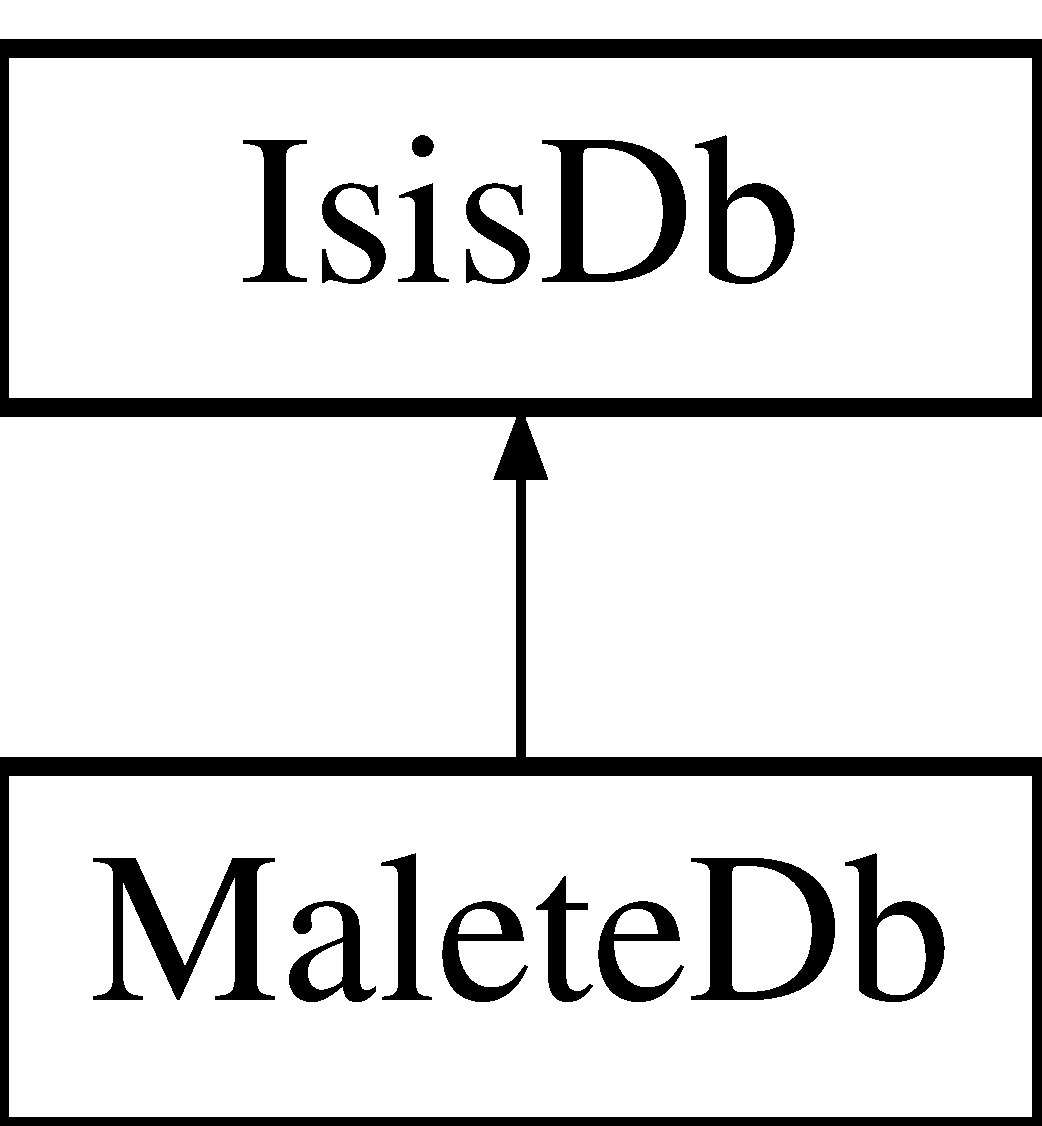
\includegraphics[height=2cm]{classMaleteDb}
\end{center}
\end{figure}
\subsection*{Public Member Functions}
\begin{DoxyCompactItemize}
\item 
\hyperlink{classMaleteDb_a60f87371bc1ec156b010e5b38b4c22e2}{\_\-\_\-construct} (\$schema)
\item 
\hyperlink{classMaleteDb_ad2a65876db24adc388afce465e0c153e}{read} (\$id)
\item 
\hyperlink{classMaleteDb_a5c6cb09a072e5d2ddce31c77098ccba4}{entries} ()
\item 
\hyperlink{classMaleteDb_a4f16c48facae498d0db1a042e9727d04}{example} ()
\item 
\hyperlink{classMaleteDb_ab2da32d84af17df79d947ae32257b4ec}{check} (\$schema, \$section=NULL)
\item 
\hyperlink{classMaleteDb_ac87c3ac1b3d9a6297be8574aa303e033}{tag} (\$results)
\item 
\hyperlink{classMaleteDb_a17562c1c53594762454d65be823fcdb5}{logger} (\$message)
\end{DoxyCompactItemize}
\subsection*{Public Attributes}
\begin{DoxyCompactItemize}
\item 
\hyperlink{classMaleteDb_af2cd60ce81381edc3ca09a6812cf79fd}{\$fdt}
\item 
\hyperlink{classMaleteDb_a4b970df3631d2763f001c96ee417f27a}{\$db}
\item 
\hyperlink{classMaleteDb_a833fed4faae9537306053ee966c06197}{\$format}
\item 
\hyperlink{classMaleteDb_ae1c8cefd1a6e661fb03c214f47336368}{\$log}
\end{DoxyCompactItemize}


\subsection{Detailed Description}
Malete implementation of \hyperlink{interfaceIsisDb}{IsisDb}.

\begin{DoxyWarning}{Warning}
This implementation is currently outdated and lacks basic functionalities such as subfield handling and therefore it's use is not recommended. 
\end{DoxyWarning}


\subsection{Constructor \& Destructor Documentation}
\hypertarget{classMaleteDb_a60f87371bc1ec156b010e5b38b4c22e2}{
\index{MaleteDb@{MaleteDb}!\_\-\_\-construct@{\_\-\_\-construct}}
\index{\_\-\_\-construct@{\_\-\_\-construct}!MaleteDb@{MaleteDb}}
\subsubsection[{\_\-\_\-construct}]{\setlength{\rightskip}{0pt plus 5cm}MaleteDb::\_\-\_\-construct (\$ {\em schema})}}
\label{classMaleteDb_a60f87371bc1ec156b010e5b38b4c22e2}
Constructor.

\begin{DoxySeeAlso}{See also}
\hyperlink{interfaceIsisDb_ae1c0a3496d55f710d34c5c19ada7a66b}{IsisDb::\_\-\_\-construct()} 
\end{DoxySeeAlso}


Implements \hyperlink{interfaceIsisDb_ae1c0a3496d55f710d34c5c19ada7a66b}{IsisDb}.



\subsection{Member Function Documentation}
\hypertarget{classMaleteDb_ab2da32d84af17df79d947ae32257b4ec}{
\index{MaleteDb@{MaleteDb}!check@{check}}
\index{check@{check}!MaleteDb@{MaleteDb}}
\subsubsection[{check}]{\setlength{\rightskip}{0pt plus 5cm}MaleteDb::check (\$ {\em schema}, \/  \$ {\em section} = {\ttfamily NULL})}}
\label{classMaleteDb_ab2da32d84af17df79d947ae32257b4ec}
Check configuration.

\begin{DoxySeeAlso}{See also}
\hyperlink{interfaceIsisDb_af681b8f990b579f1835aa7ba4c83f1b8}{IsisDb::check()} 
\end{DoxySeeAlso}


Implements \hyperlink{interfaceIsisDb_af681b8f990b579f1835aa7ba4c83f1b8}{IsisDb}.

\hypertarget{classMaleteDb_a5c6cb09a072e5d2ddce31c77098ccba4}{
\index{MaleteDb@{MaleteDb}!entries@{entries}}
\index{entries@{entries}!MaleteDb@{MaleteDb}}
\subsubsection[{entries}]{\setlength{\rightskip}{0pt plus 5cm}MaleteDb::entries ()}}
\label{classMaleteDb_a5c6cb09a072e5d2ddce31c77098ccba4}
Return number of entries in the database.

The Malete API doen't implement such feature so we have to emulate it by iterating over all entries until \hyperlink{classMaleteDb_ad2a65876db24adc388afce465e0c153e}{MaleteDb::read()} returns FALSE.

\begin{DoxySeeAlso}{See also}
\hyperlink{interfaceIsisDb_a86f38eca2b6d0835b60770d8a4e511ff}{IsisDb::entries()} 
\end{DoxySeeAlso}


Implements \hyperlink{interfaceIsisDb_a86f38eca2b6d0835b60770d8a4e511ff}{IsisDb}.

\hypertarget{classMaleteDb_a4f16c48facae498d0db1a042e9727d04}{
\index{MaleteDb@{MaleteDb}!example@{example}}
\index{example@{example}!MaleteDb@{MaleteDb}}
\subsubsection[{example}]{\setlength{\rightskip}{0pt plus 5cm}MaleteDb::example ()}}
\label{classMaleteDb_a4f16c48facae498d0db1a042e9727d04}
Return an example schema.

\begin{DoxySeeAlso}{See also}
\hyperlink{interfaceIsisDb_a857c10d90da64067efa17afb2f32edb6}{IsisDb::example()} 
\end{DoxySeeAlso}


Implements \hyperlink{interfaceIsisDb_a857c10d90da64067efa17afb2f32edb6}{IsisDb}.

\hypertarget{classMaleteDb_a17562c1c53594762454d65be823fcdb5}{
\index{MaleteDb@{MaleteDb}!logger@{logger}}
\index{logger@{logger}!MaleteDb@{MaleteDb}}
\subsubsection[{logger}]{\setlength{\rightskip}{0pt plus 5cm}MaleteDb::logger (\$ {\em message})}}
\label{classMaleteDb_a17562c1c53594762454d65be823fcdb5}
Class logger.


\begin{DoxyParams}{Parameters}
\item[{\em \$message}]Log message. \end{DoxyParams}
\hypertarget{classMaleteDb_ad2a65876db24adc388afce465e0c153e}{
\index{MaleteDb@{MaleteDb}!read@{read}}
\index{read@{read}!MaleteDb@{MaleteDb}}
\subsubsection[{read}]{\setlength{\rightskip}{0pt plus 5cm}MaleteDb::read (\$ {\em id})}}
\label{classMaleteDb_ad2a65876db24adc388afce465e0c153e}
Read an entry.

\begin{DoxySeeAlso}{See also}
\hyperlink{interfaceIsisDb_a68335ec0db01ef03f0725621b38b5686}{IsisDb::read()}
\end{DoxySeeAlso}
\begin{Desc}
\item[\hyperlink{todo__todo000002}{Todo}]Subfield handling. \end{Desc}


Implements \hyperlink{interfaceIsisDb_a68335ec0db01ef03f0725621b38b5686}{IsisDb}.

\hypertarget{classMaleteDb_ac87c3ac1b3d9a6297be8574aa303e033}{
\index{MaleteDb@{MaleteDb}!tag@{tag}}
\index{tag@{tag}!MaleteDb@{MaleteDb}}
\subsubsection[{tag}]{\setlength{\rightskip}{0pt plus 5cm}MaleteDb::tag (\$ {\em results})}}
\label{classMaleteDb_ac87c3ac1b3d9a6297be8574aa303e033}
Tag results of a db query.

This function converts the keys of query result from field numbers to names and and also puts repetition fields into place as Malete deals with field repetition by using a 'tag' property in the resulting query object.


\begin{DoxyParams}{Parameters}
\item[{\em \$results}]Database query results.\end{DoxyParams}
\begin{DoxyReturn}{Returns}
Tagged database result. 
\end{DoxyReturn}


\subsection{Member Data Documentation}
\hypertarget{classMaleteDb_a4b970df3631d2763f001c96ee417f27a}{
\index{MaleteDb@{MaleteDb}!\$db@{\$db}}
\index{\$db@{\$db}!MaleteDb@{MaleteDb}}
\subsubsection[{\$db}]{\setlength{\rightskip}{0pt plus 5cm}MaleteDb::\$db}}
\label{classMaleteDb_a4b970df3631d2763f001c96ee417f27a}
Database resource. \hypertarget{classMaleteDb_af2cd60ce81381edc3ca09a6812cf79fd}{
\index{MaleteDb@{MaleteDb}!\$fdt@{\$fdt}}
\index{\$fdt@{\$fdt}!MaleteDb@{MaleteDb}}
\subsubsection[{\$fdt}]{\setlength{\rightskip}{0pt plus 5cm}MaleteDb::\$fdt}}
\label{classMaleteDb_af2cd60ce81381edc3ca09a6812cf79fd}
Field description table. \hypertarget{classMaleteDb_a833fed4faae9537306053ee966c06197}{
\index{MaleteDb@{MaleteDb}!\$format@{\$format}}
\index{\$format@{\$format}!MaleteDb@{MaleteDb}}
\subsubsection[{\$format}]{\setlength{\rightskip}{0pt plus 5cm}MaleteDb::\$format}}
\label{classMaleteDb_a833fed4faae9537306053ee966c06197}
Database format, derived from \$schema. \hypertarget{classMaleteDb_ae1c8cefd1a6e661fb03c214f47336368}{
\index{MaleteDb@{MaleteDb}!\$log@{\$log}}
\index{\$log@{\$log}!MaleteDb@{MaleteDb}}
\subsubsection[{\$log}]{\setlength{\rightskip}{0pt plus 5cm}MaleteDb::\$log}}
\label{classMaleteDb_ae1c8cefd1a6e661fb03c214f47336368}
Class action log. 

The documentation for this class was generated from the following file:\begin{DoxyCompactItemize}
\item 
classes/backends/MaleteDb.php\end{DoxyCompactItemize}

\hypertarget{classPhpIsisDb}{
\section{PhpIsisDb Class Reference}
\label{classPhpIsisDb}\index{PhpIsisDb@{PhpIsisDb}}
}
Inheritance diagram for PhpIsisDb:\begin{figure}[H]
\begin{center}
\leavevmode
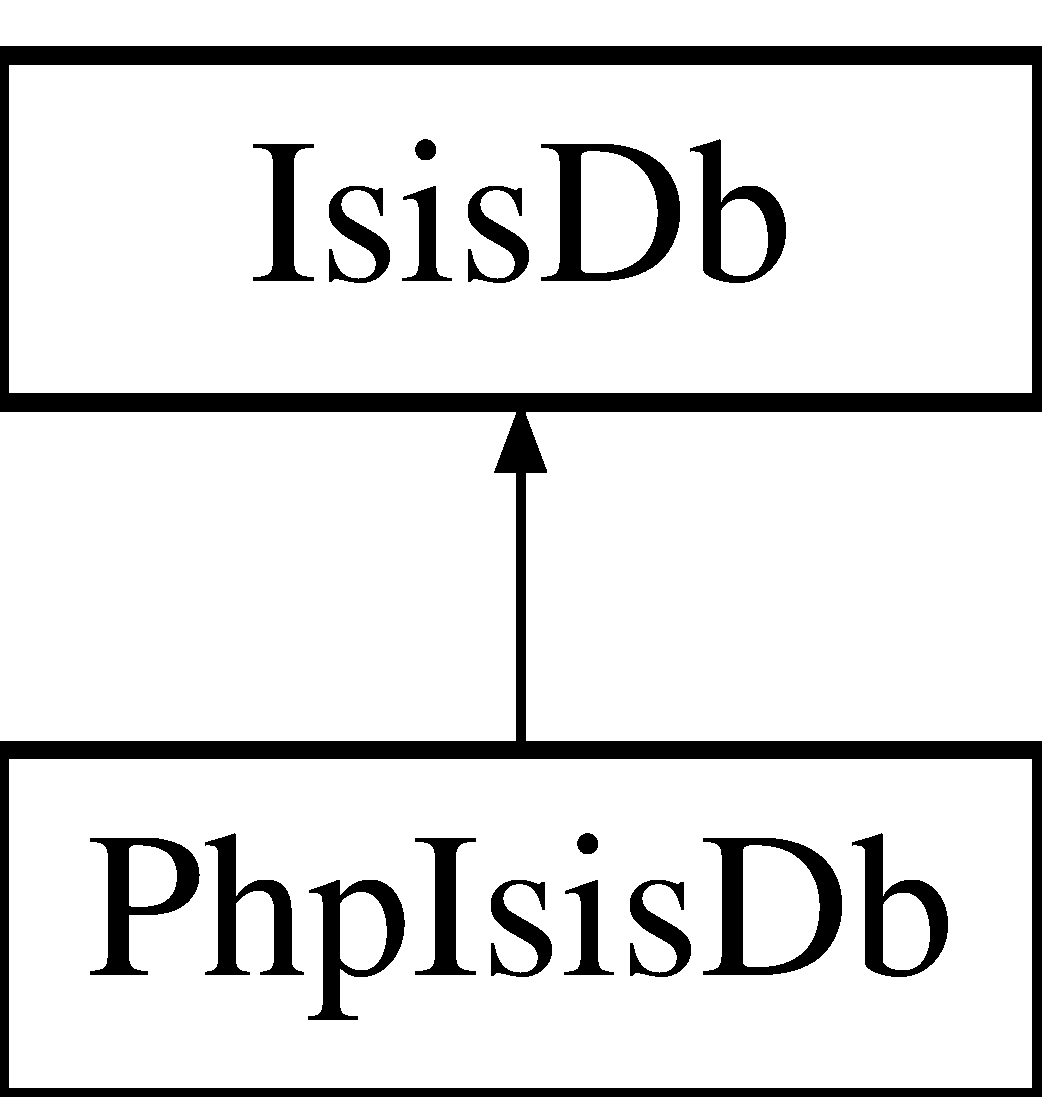
\includegraphics[height=2.000000cm]{classPhpIsisDb}
\end{center}
\end{figure}
\subsection*{Public Member Functions}
\begin{DoxyCompactItemize}
\item 
\hyperlink{classPhpIsisDb_abb6db51373d065baf9135fd278653bc5}{\_\-\_\-construct} (\$schema)
\item 
\hyperlink{classPhpIsisDb_af2266931746f6f2335b831be8b8333fb}{read} (\$id)
\item 
\hyperlink{classPhpIsisDb_a0491ce84e5a85e775f811f18e63ef0fb}{entries} ()
\item 
\hyperlink{classPhpIsisDb_a7f4f3a9fd6dab86bd3cb3149d65f92cd}{example} ()
\item 
\hyperlink{classPhpIsisDb_a849f238c3323f53431be1c225a914d98}{tag} (\$results)
\item 
\hyperlink{classPhpIsisDb_a46f8c39b305f170e2cf8ae5f4d218e74}{charset} (\&\$data)
\item 
\hyperlink{classPhpIsisDb_a8d8185060a26d4fe673844b2ea3db39a}{logger} (\$message)
\end{DoxyCompactItemize}
\subsection*{Static Public Member Functions}
\begin{DoxyCompactItemize}
\item 
static \hyperlink{classPhpIsisDb_a23761cc04114090a2863467b2accc80a}{check} (\$schema, \$section=NULL)
\end{DoxyCompactItemize}
\subsection*{Public Attributes}
\begin{DoxyCompactItemize}
\item 
\hyperlink{classPhpIsisDb_a536e4c67dda71a7c7dad9ffbac299f9b}{\$db}
\item 
\hyperlink{classPhpIsisDb_a275e29f3711d37fc67cea340b564ddf3}{\$format}
\item 
\hyperlink{classPhpIsisDb_a0742105b3efab477fda99cd0561f98c7}{\$log}
\end{DoxyCompactItemize}


\subsection{Detailed Description}
PHP-\/Isis implementation of \hyperlink{interfaceIsisDb}{IsisDb}.

\begin{DoxyWarning}{Warning}
This implementation is currently outdated and lacks basic functionalities such as subfield handling and therefore it's use is not recommended. 
\end{DoxyWarning}


\subsection{Constructor \& Destructor Documentation}
\hypertarget{classPhpIsisDb_abb6db51373d065baf9135fd278653bc5}{
\index{PhpIsisDb@{PhpIsisDb}!\_\-\_\-construct@{\_\-\_\-construct}}
\index{\_\-\_\-construct@{\_\-\_\-construct}!PhpIsisDb@{PhpIsisDb}}
\subsubsection[{\_\-\_\-construct}]{\setlength{\rightskip}{0pt plus 5cm}PhpIsisDb::\_\-\_\-construct (
\begin{DoxyParamCaption}
\item[{\$}]{ schema}
\end{DoxyParamCaption}
)}}
\label{classPhpIsisDb_abb6db51373d065baf9135fd278653bc5}
Constructor.

\begin{DoxySeeAlso}{See also}
\hyperlink{interfaceIsisDb_ae1c0a3496d55f710d34c5c19ada7a66b}{IsisDb::\_\-\_\-construct()} 
\end{DoxySeeAlso}


Implements \hyperlink{interfaceIsisDb_ae1c0a3496d55f710d34c5c19ada7a66b}{IsisDb}.



\subsection{Member Function Documentation}
\hypertarget{classPhpIsisDb_a46f8c39b305f170e2cf8ae5f4d218e74}{
\index{PhpIsisDb@{PhpIsisDb}!charset@{charset}}
\index{charset@{charset}!PhpIsisDb@{PhpIsisDb}}
\subsubsection[{charset}]{\setlength{\rightskip}{0pt plus 5cm}PhpIsisDb::charset (
\begin{DoxyParamCaption}
\item[{\&\$}]{ data}
\end{DoxyParamCaption}
)}}
\label{classPhpIsisDb_a46f8c39b305f170e2cf8ae5f4d218e74}
Charset conversion.

Converts a string from the database charset to UTF-\/8.


\begin{DoxyParams}{Parameters}
\item[{\em \$data}]String to be converted.\end{DoxyParams}
\begin{DoxyReturn}{Returns}
String converted to UTF-\/8. 
\end{DoxyReturn}
\hypertarget{classPhpIsisDb_a23761cc04114090a2863467b2accc80a}{
\index{PhpIsisDb@{PhpIsisDb}!check@{check}}
\index{check@{check}!PhpIsisDb@{PhpIsisDb}}
\subsubsection[{check}]{\setlength{\rightskip}{0pt plus 5cm}static PhpIsisDb::check (
\begin{DoxyParamCaption}
\item[{\$}]{ schema, }
\item[{\$}]{ section = {\ttfamily NULL}}
\end{DoxyParamCaption}
)\hspace{0.3cm}{\ttfamily  \mbox{[}static\mbox{]}}}}
\label{classPhpIsisDb_a23761cc04114090a2863467b2accc80a}
Check configuration.

\begin{DoxySeeAlso}{See also}
\hyperlink{interfaceIsisDb_af681b8f990b579f1835aa7ba4c83f1b8}{IsisDb::check()} 
\end{DoxySeeAlso}


Implements \hyperlink{interfaceIsisDb_af681b8f990b579f1835aa7ba4c83f1b8}{IsisDb}.

\hypertarget{classPhpIsisDb_a0491ce84e5a85e775f811f18e63ef0fb}{
\index{PhpIsisDb@{PhpIsisDb}!entries@{entries}}
\index{entries@{entries}!PhpIsisDb@{PhpIsisDb}}
\subsubsection[{entries}]{\setlength{\rightskip}{0pt plus 5cm}PhpIsisDb::entries (
\begin{DoxyParamCaption}
{}
\end{DoxyParamCaption}
)}}
\label{classPhpIsisDb_a0491ce84e5a85e775f811f18e63ef0fb}
Return number of entries in the database.

\begin{DoxySeeAlso}{See also}
\hyperlink{interfaceIsisDb_a86f38eca2b6d0835b60770d8a4e511ff}{IsisDb::entries()} 
\end{DoxySeeAlso}


Implements \hyperlink{interfaceIsisDb_a86f38eca2b6d0835b60770d8a4e511ff}{IsisDb}.

\hypertarget{classPhpIsisDb_a7f4f3a9fd6dab86bd3cb3149d65f92cd}{
\index{PhpIsisDb@{PhpIsisDb}!example@{example}}
\index{example@{example}!PhpIsisDb@{PhpIsisDb}}
\subsubsection[{example}]{\setlength{\rightskip}{0pt plus 5cm}PhpIsisDb::example (
\begin{DoxyParamCaption}
{}
\end{DoxyParamCaption}
)}}
\label{classPhpIsisDb_a7f4f3a9fd6dab86bd3cb3149d65f92cd}
Return an example schema.

\begin{DoxySeeAlso}{See also}
\hyperlink{interfaceIsisDb_a857c10d90da64067efa17afb2f32edb6}{IsisDb::example()} 
\end{DoxySeeAlso}


Implements \hyperlink{interfaceIsisDb_a857c10d90da64067efa17afb2f32edb6}{IsisDb}.

\hypertarget{classPhpIsisDb_a8d8185060a26d4fe673844b2ea3db39a}{
\index{PhpIsisDb@{PhpIsisDb}!logger@{logger}}
\index{logger@{logger}!PhpIsisDb@{PhpIsisDb}}
\subsubsection[{logger}]{\setlength{\rightskip}{0pt plus 5cm}PhpIsisDb::logger (
\begin{DoxyParamCaption}
\item[{\$}]{ message}
\end{DoxyParamCaption}
)}}
\label{classPhpIsisDb_a8d8185060a26d4fe673844b2ea3db39a}
Class logger.


\begin{DoxyParams}{Parameters}
\item[{\em \$message}]Log message. \end{DoxyParams}
\hypertarget{classPhpIsisDb_af2266931746f6f2335b831be8b8333fb}{
\index{PhpIsisDb@{PhpIsisDb}!read@{read}}
\index{read@{read}!PhpIsisDb@{PhpIsisDb}}
\subsubsection[{read}]{\setlength{\rightskip}{0pt plus 5cm}PhpIsisDb::read (
\begin{DoxyParamCaption}
\item[{\$}]{ id}
\end{DoxyParamCaption}
)}}
\label{classPhpIsisDb_af2266931746f6f2335b831be8b8333fb}
Read an entry.

The PHP-\/Isis API doen't implement such feature so we have to emulate it by geting all entries and using isis\_\-data\_\-seek() to get the desired record.

\begin{DoxySeeAlso}{See also}
\hyperlink{interfaceIsisDb_a68335ec0db01ef03f0725621b38b5686}{IsisDb::read()}
\end{DoxySeeAlso}
\begin{Desc}
\item[\hyperlink{todo__todo000003}{Todo}]Subfield handling. \end{Desc}


Implements \hyperlink{interfaceIsisDb_a68335ec0db01ef03f0725621b38b5686}{IsisDb}.

\hypertarget{classPhpIsisDb_a849f238c3323f53431be1c225a914d98}{
\index{PhpIsisDb@{PhpIsisDb}!tag@{tag}}
\index{tag@{tag}!PhpIsisDb@{PhpIsisDb}}
\subsubsection[{tag}]{\setlength{\rightskip}{0pt plus 5cm}PhpIsisDb::tag (
\begin{DoxyParamCaption}
\item[{\$}]{ results}
\end{DoxyParamCaption}
)}}
\label{classPhpIsisDb_a849f238c3323f53431be1c225a914d98}
Tag results of a db query.

This function converts the keys of query result from field numbers to names.


\begin{DoxyParams}{Parameters}
\item[{\em \$results}]Database query results.\end{DoxyParams}
\begin{DoxyReturn}{Returns}
Tagged database result. 
\end{DoxyReturn}


\subsection{Member Data Documentation}
\hypertarget{classPhpIsisDb_a536e4c67dda71a7c7dad9ffbac299f9b}{
\index{PhpIsisDb@{PhpIsisDb}!\$db@{\$db}}
\index{\$db@{\$db}!PhpIsisDb@{PhpIsisDb}}
\subsubsection[{\$db}]{\setlength{\rightskip}{0pt plus 5cm}PhpIsisDb::\$db}}
\label{classPhpIsisDb_a536e4c67dda71a7c7dad9ffbac299f9b}
Database resource. \hypertarget{classPhpIsisDb_a275e29f3711d37fc67cea340b564ddf3}{
\index{PhpIsisDb@{PhpIsisDb}!\$format@{\$format}}
\index{\$format@{\$format}!PhpIsisDb@{PhpIsisDb}}
\subsubsection[{\$format}]{\setlength{\rightskip}{0pt plus 5cm}PhpIsisDb::\$format}}
\label{classPhpIsisDb_a275e29f3711d37fc67cea340b564ddf3}
Database format, derived from \$schema. \hypertarget{classPhpIsisDb_a0742105b3efab477fda99cd0561f98c7}{
\index{PhpIsisDb@{PhpIsisDb}!\$log@{\$log}}
\index{\$log@{\$log}!PhpIsisDb@{PhpIsisDb}}
\subsubsection[{\$log}]{\setlength{\rightskip}{0pt plus 5cm}PhpIsisDb::\$log}}
\label{classPhpIsisDb_a0742105b3efab477fda99cd0561f98c7}
Class action log. 

The documentation for this class was generated from the following file:\begin{DoxyCompactItemize}
\item 
classes/backends/PhpIsisDb.php\end{DoxyCompactItemize}

\hypertarget{classSchemaDb}{
\section{SchemaDb Class Reference}
\label{classSchemaDb}\index{SchemaDb@{SchemaDb}}
}
\subsection*{Public Member Functions}
\begin{DoxyCompactItemize}
\item 
\hyperlink{classSchemaDb_af5c9271759bed2f9cccc80a05f7c5da8}{optional} ()
\item 
\hyperlink{classSchemaDb_a923a94169459c4dee3f74000b4aa1807}{example} ()
\end{DoxyCompactItemize}
\subsection*{Static Public Member Functions}
\begin{DoxyCompactItemize}
\item 
static \hyperlink{classSchemaDb_a31db21bccb179162b5bb02b14b72d3e3}{required} ()
\item 
static \hyperlink{classSchemaDb_a42acc85b08a20b121204b1caf3a83e61}{check} (\$schema, \$section=NULL)
\end{DoxyCompactItemize}


\subsection{Detailed Description}
\hyperlink{classSchemaDb}{SchemaDb} class with standard database procedures and configuration. 

\subsection{Member Function Documentation}
\hypertarget{classSchemaDb_a42acc85b08a20b121204b1caf3a83e61}{
\index{SchemaDb@{SchemaDb}!check@{check}}
\index{check@{check}!SchemaDb@{SchemaDb}}
\subsubsection[{check}]{\setlength{\rightskip}{0pt plus 5cm}static SchemaDb::check (
\begin{DoxyParamCaption}
\item[{\$}]{ schema, }
\item[{\$}]{ section = {\ttfamily NULL}}
\end{DoxyParamCaption}
)\hspace{0.3cm}{\ttfamily  \mbox{[}static\mbox{]}}}}
\label{classSchemaDb_a42acc85b08a20b121204b1caf3a83e61}
Recursively check for required fields in a database schema.

\begin{DoxySeeAlso}{See also}
\hyperlink{interfaceIsisDb_af681b8f990b579f1835aa7ba4c83f1b8}{IsisDb::check()} 
\end{DoxySeeAlso}
\hypertarget{classSchemaDb_a923a94169459c4dee3f74000b4aa1807}{
\index{SchemaDb@{SchemaDb}!example@{example}}
\index{example@{example}!SchemaDb@{SchemaDb}}
\subsubsection[{example}]{\setlength{\rightskip}{0pt plus 5cm}SchemaDb::example (
\begin{DoxyParamCaption}
{}
\end{DoxyParamCaption}
)}}
\label{classSchemaDb_a923a94169459c4dee3f74000b4aa1807}
Return an example database schema.

\begin{DoxySeeAlso}{See also}
\hyperlink{interfaceIsisDb_a857c10d90da64067efa17afb2f32edb6}{IsisDb::example()} 
\end{DoxySeeAlso}
\hypertarget{classSchemaDb_af5c9271759bed2f9cccc80a05f7c5da8}{
\index{SchemaDb@{SchemaDb}!optional@{optional}}
\index{optional@{optional}!SchemaDb@{SchemaDb}}
\subsubsection[{optional}]{\setlength{\rightskip}{0pt plus 5cm}SchemaDb::optional (
\begin{DoxyParamCaption}
{}
\end{DoxyParamCaption}
)}}
\label{classSchemaDb_af5c9271759bed2f9cccc80a05f7c5da8}
Return the optional database config.

\begin{DoxyReturn}{Returns}
Array with optional config. 
\end{DoxyReturn}
\hypertarget{classSchemaDb_a31db21bccb179162b5bb02b14b72d3e3}{
\index{SchemaDb@{SchemaDb}!required@{required}}
\index{required@{required}!SchemaDb@{SchemaDb}}
\subsubsection[{required}]{\setlength{\rightskip}{0pt plus 5cm}static SchemaDb::required (
\begin{DoxyParamCaption}
{}
\end{DoxyParamCaption}
)\hspace{0.3cm}{\ttfamily  \mbox{[}static\mbox{]}}}}
\label{classSchemaDb_a31db21bccb179162b5bb02b14b72d3e3}
Return the required database config.

\begin{DoxyReturn}{Returns}
Array with required config. 
\end{DoxyReturn}


The documentation for this class was generated from the following file:\begin{DoxyCompactItemize}
\item 
classes/backends/SchemaDb.php\end{DoxyCompactItemize}

\printindex
\end{document}
